\chapter{Auxiliary Information}

\section{\ac{tmh}: \ac{dea} Results} \label{sec:tabminhash_results}

\begin{figure}[H]
    \centering
    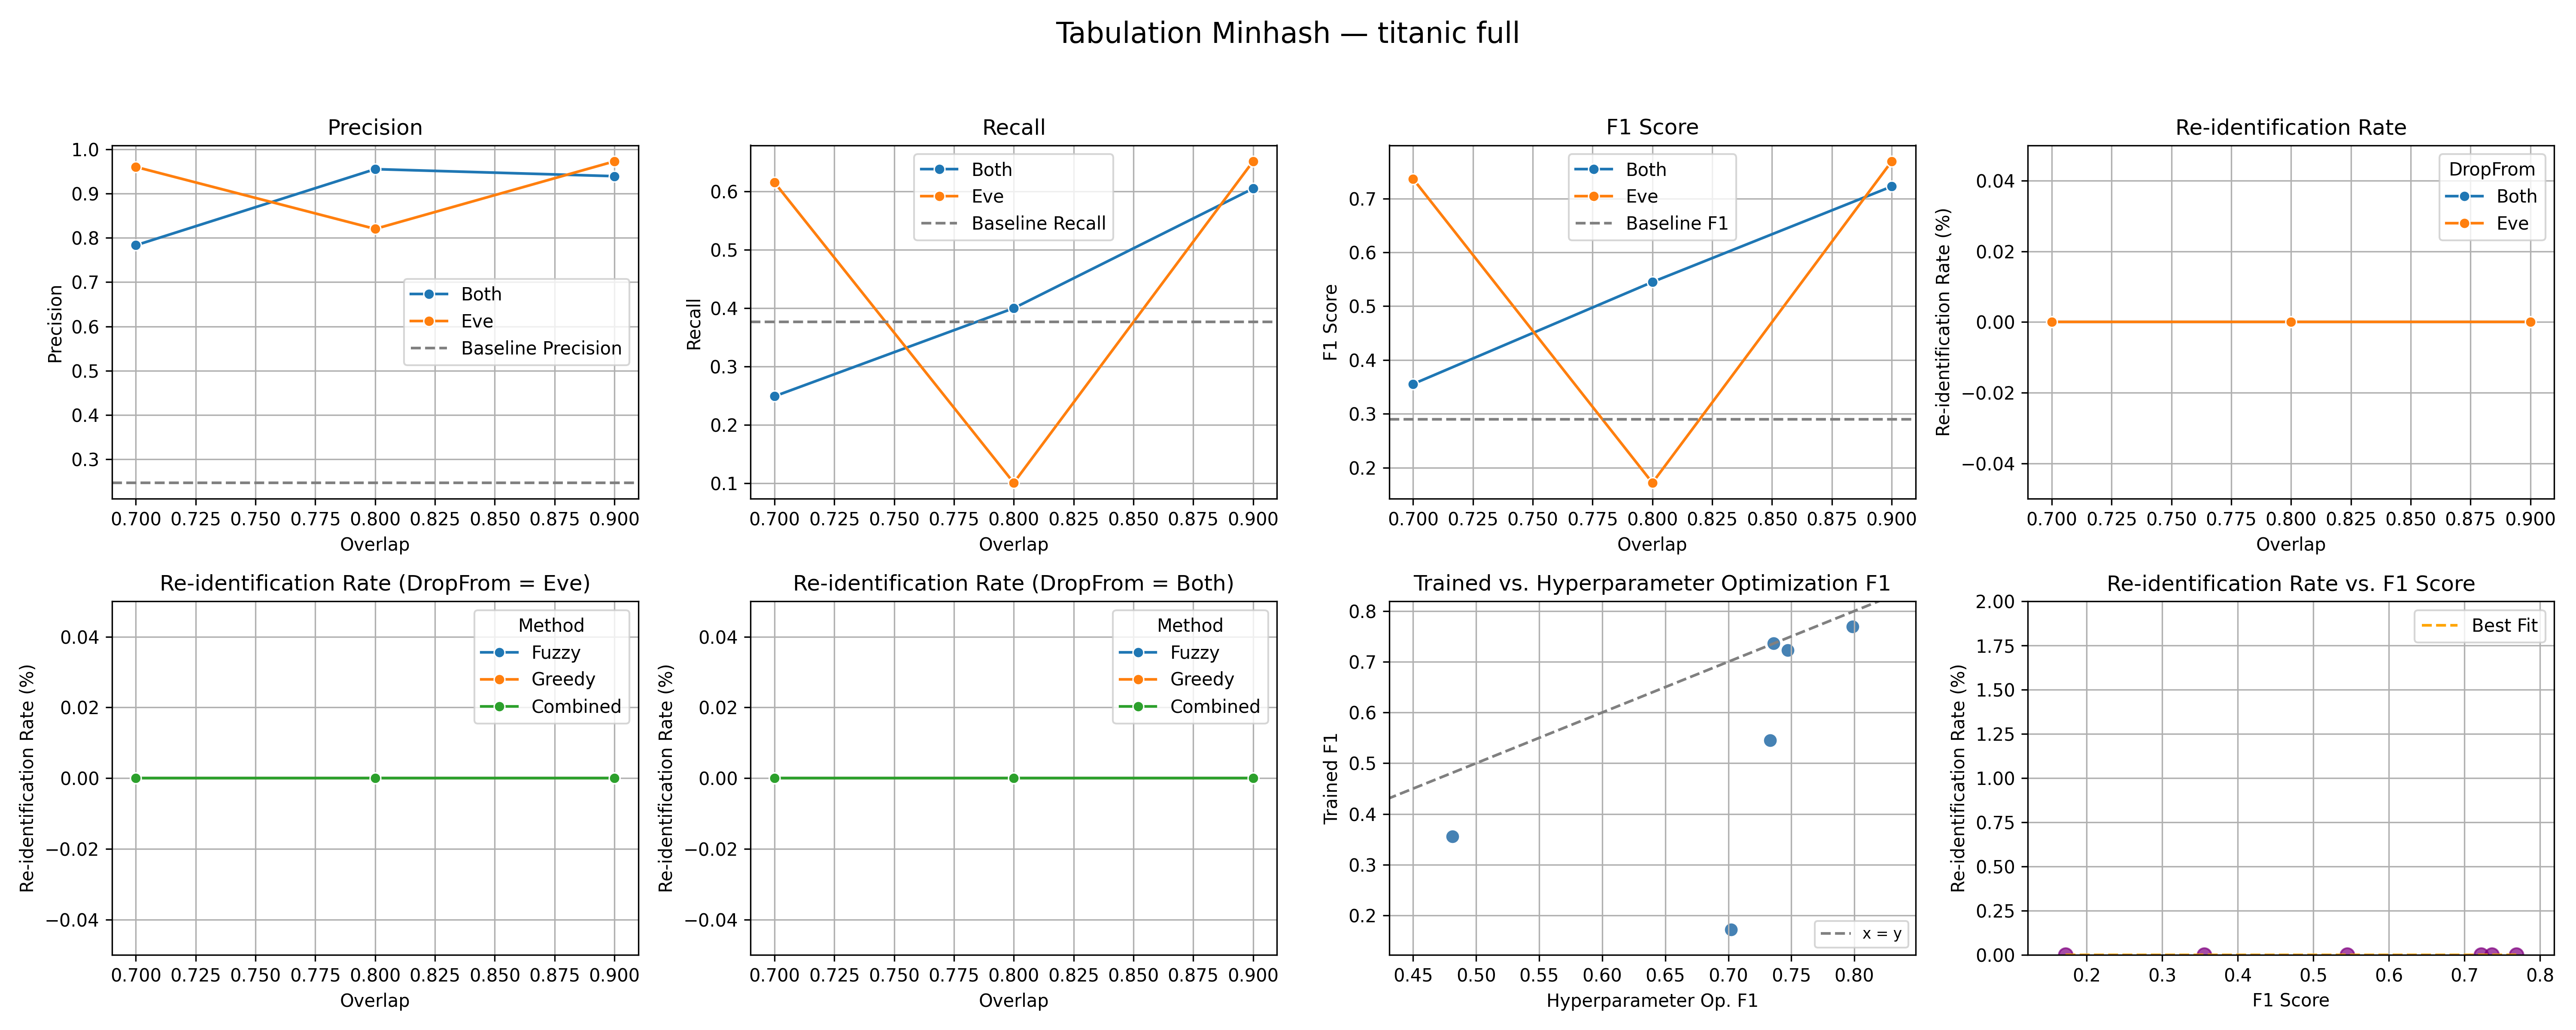
\includegraphics[width=\textwidth]{figures/TabMinHash_titanic_full_metrics.png}
    \caption{\ac{tmh} results on the \texttt{titanic\_full} dataset.}
    \label{fig:tabminhash_titanic}
\end{figure}

\begin{figure}[H]
    \centering
    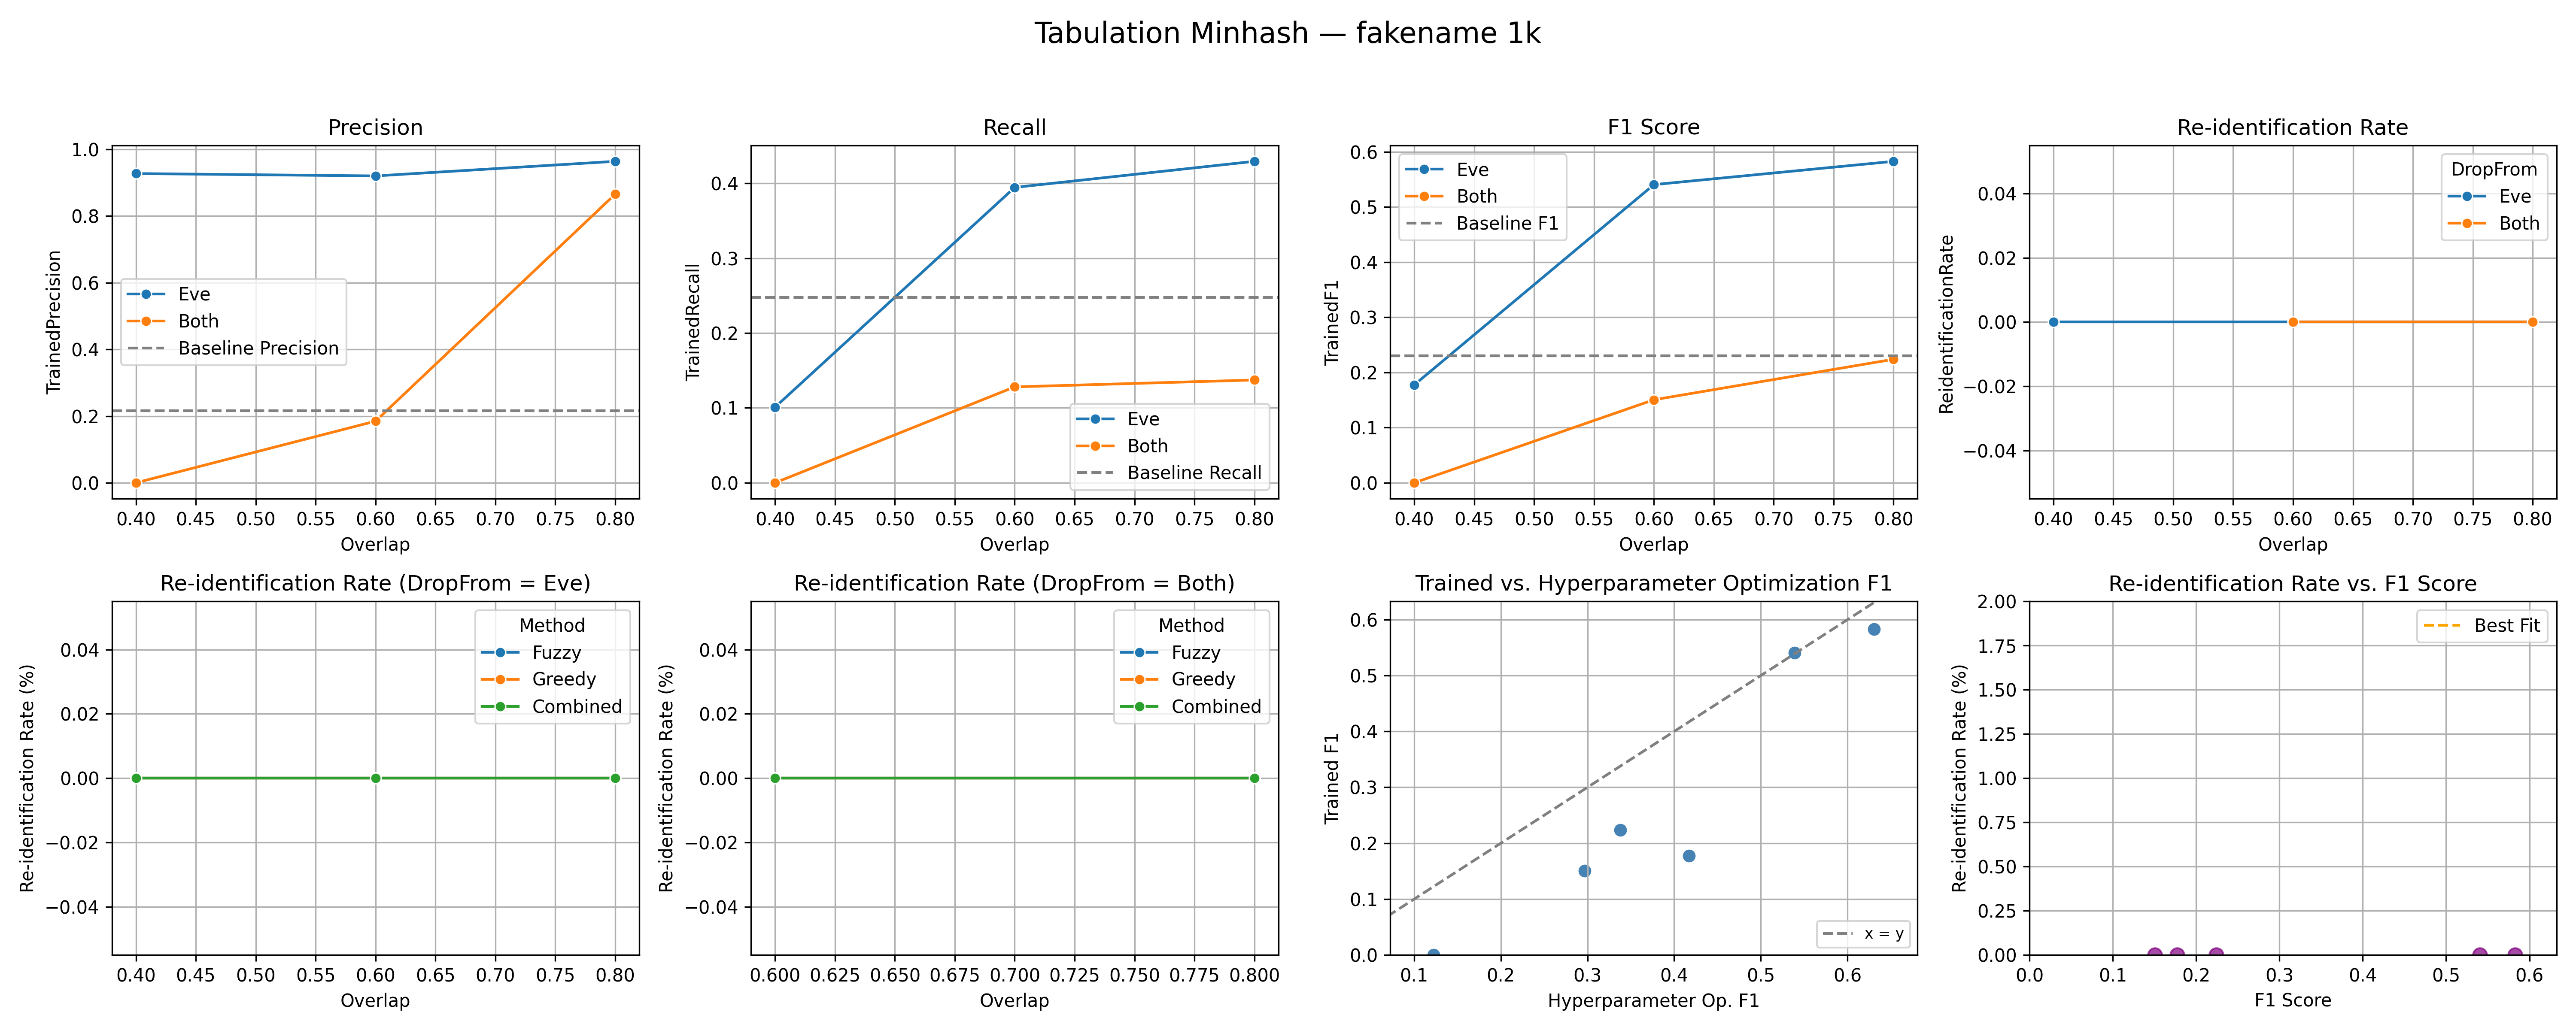
\includegraphics[width=\textwidth]{figures/TabMinHash_fakename_1k_metrics.png}
    \caption{\ac{tmh} results on the \texttt{fakename\_1k} dataset.}
    \label{fig:tabminhash_fakename1k}
\end{figure}

\begin{figure}[H]
    \centering
    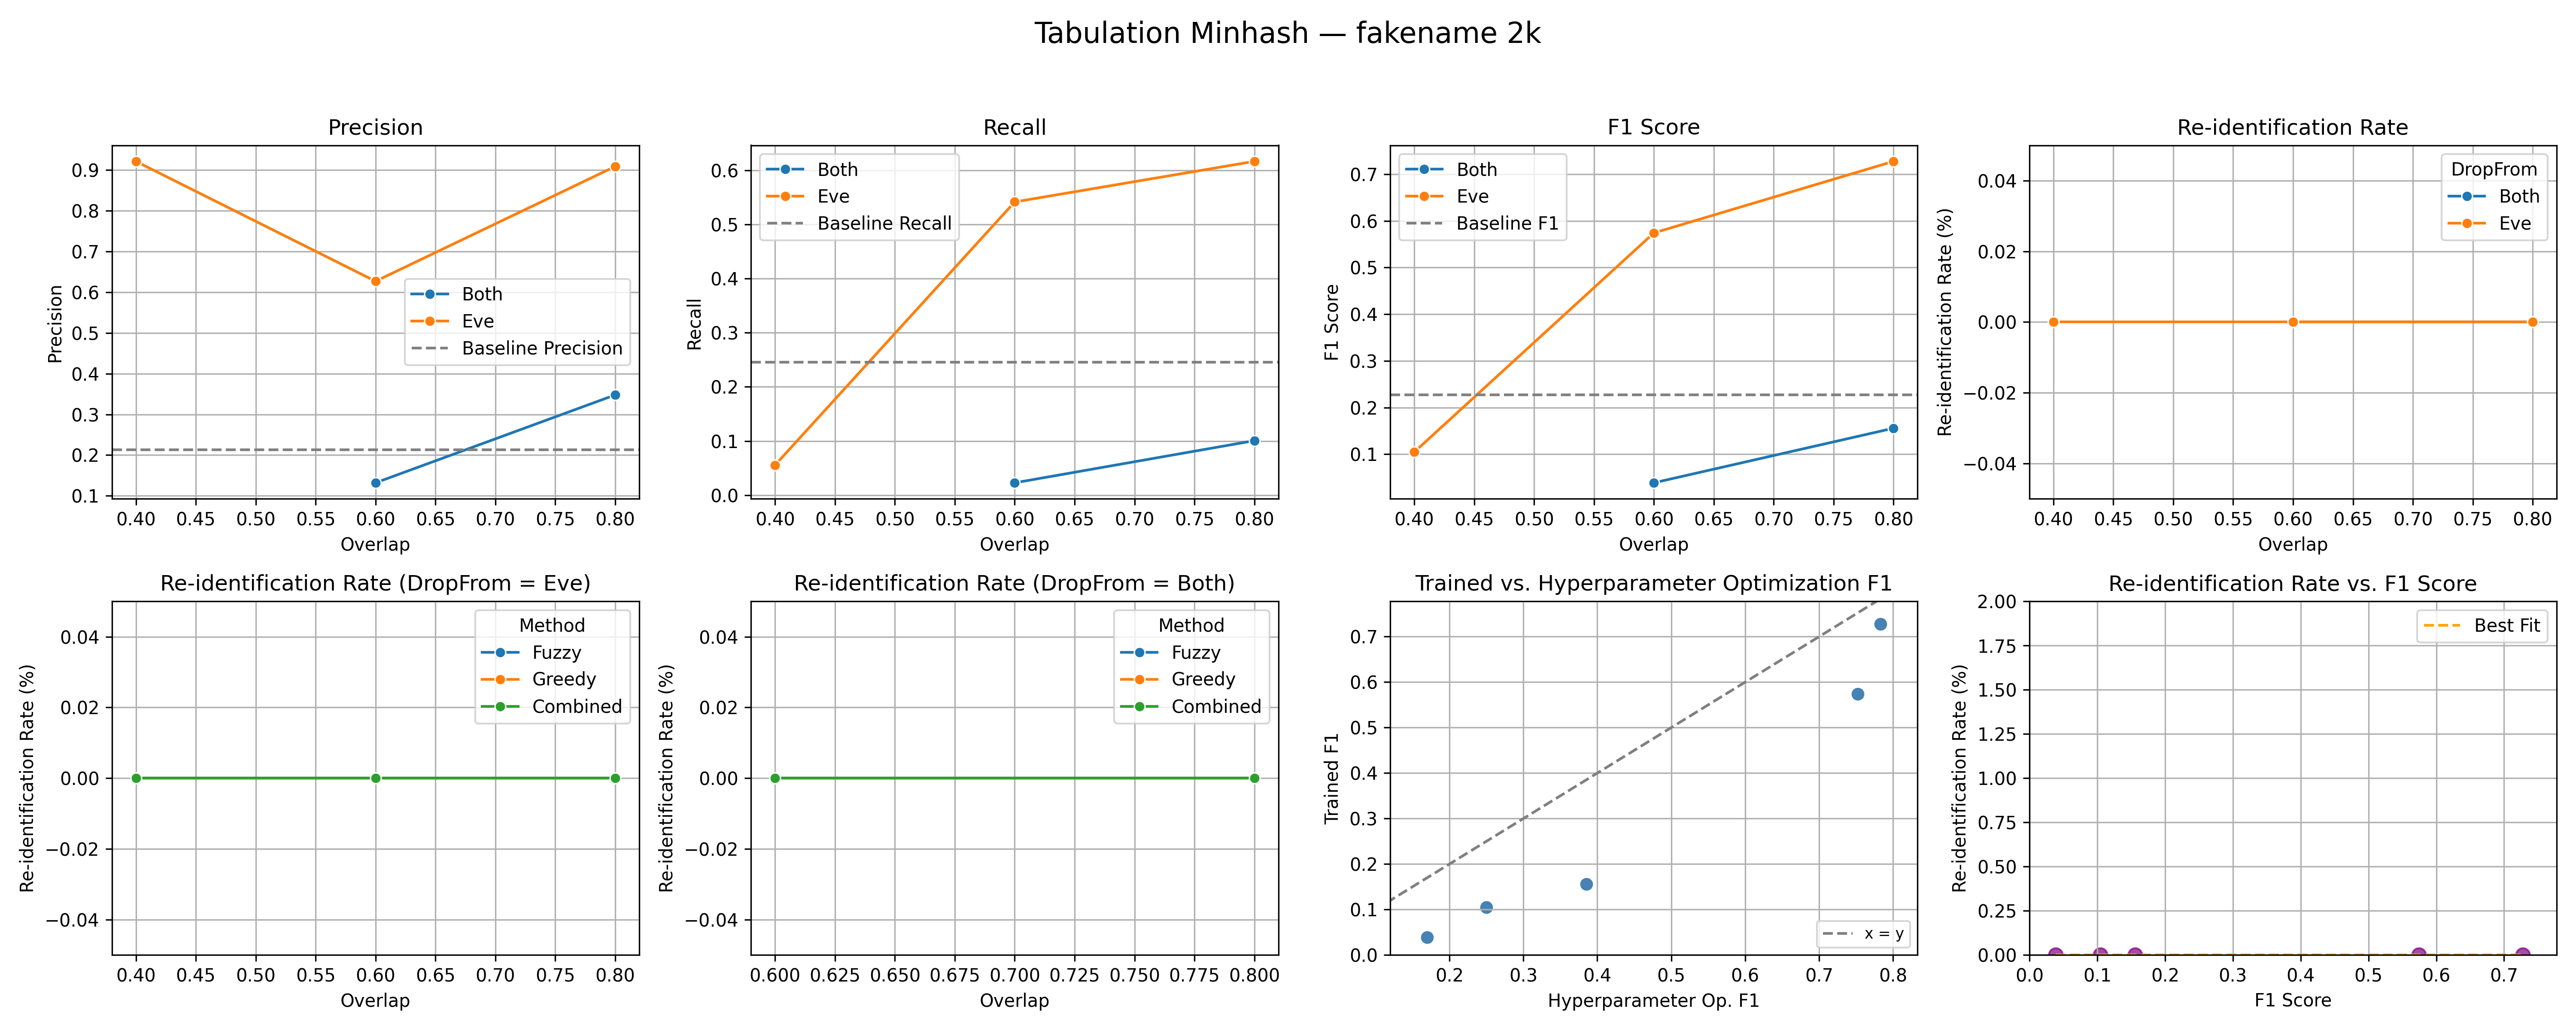
\includegraphics[width=\textwidth]{figures/TabMinHash_fakename_2k_metrics.png}
    \caption{\ac{tmh} results on the \texttt{fakename\_2k} dataset.}
    \label{fig:tabminhash_fakename2k}
\end{figure}

\begin{figure}[H]
    \centering
    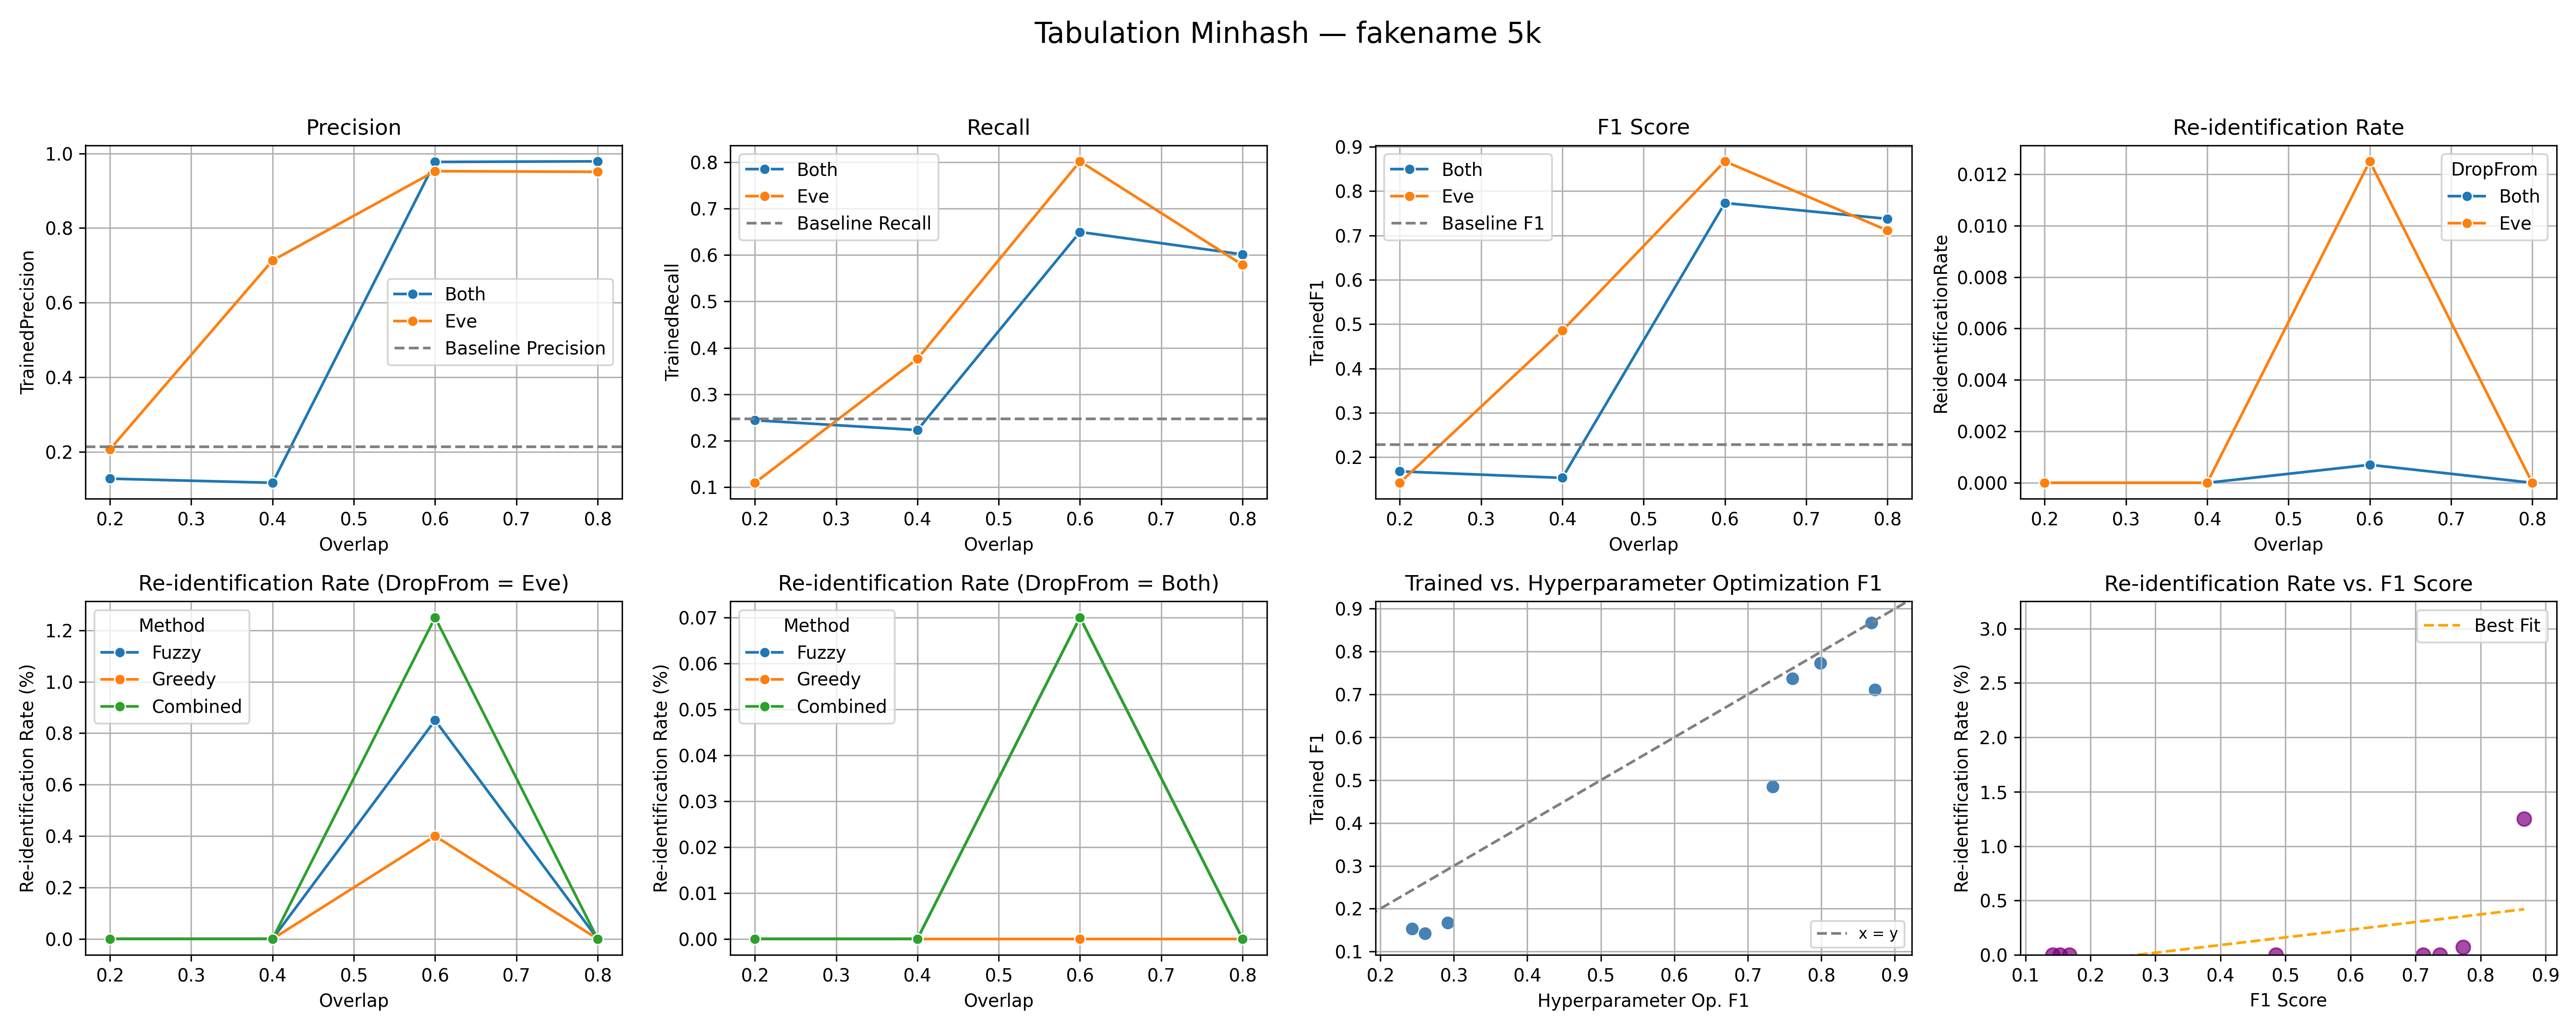
\includegraphics[width=\textwidth]{figures/TabMinHash_fakename_5k_metrics.png}
    \caption{\ac{tmh} results on the \texttt{fakename\_5k} dataset.}
    \label{fig:tabminhash_fakename5k}
\end{figure}

\begin{figure}[H]
    \centering
    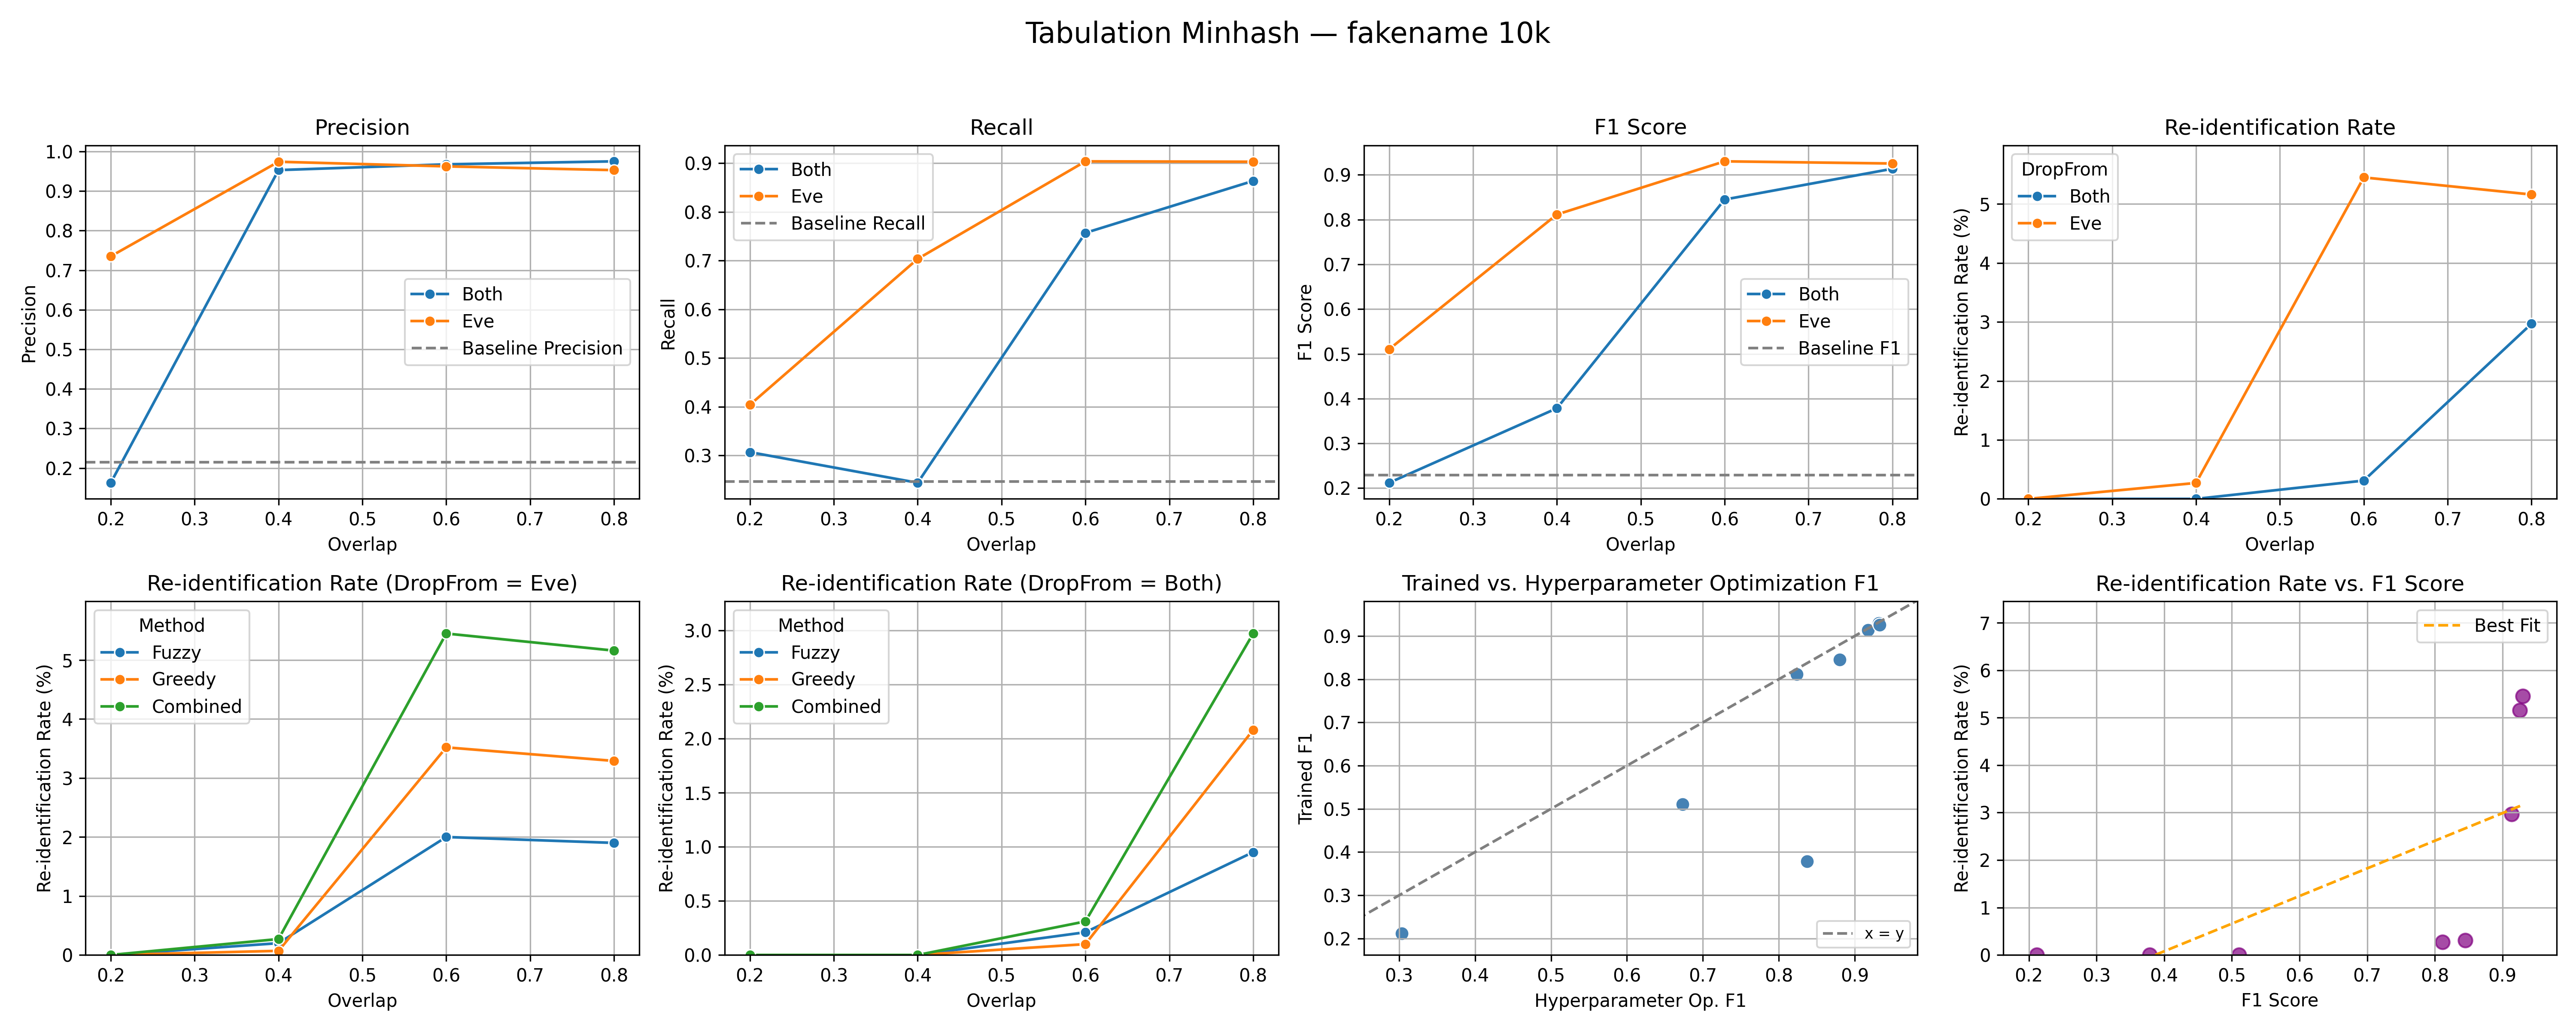
\includegraphics[width=\textwidth]{figures/TabMinHash_fakename_10k_metrics.png}
    \caption{\ac{tmh} results on the \texttt{fakename\_10k} dataset.}
    \label{fig:tabminhash_fakename10k}
\end{figure}

\begin{figure}[H]
    \centering
    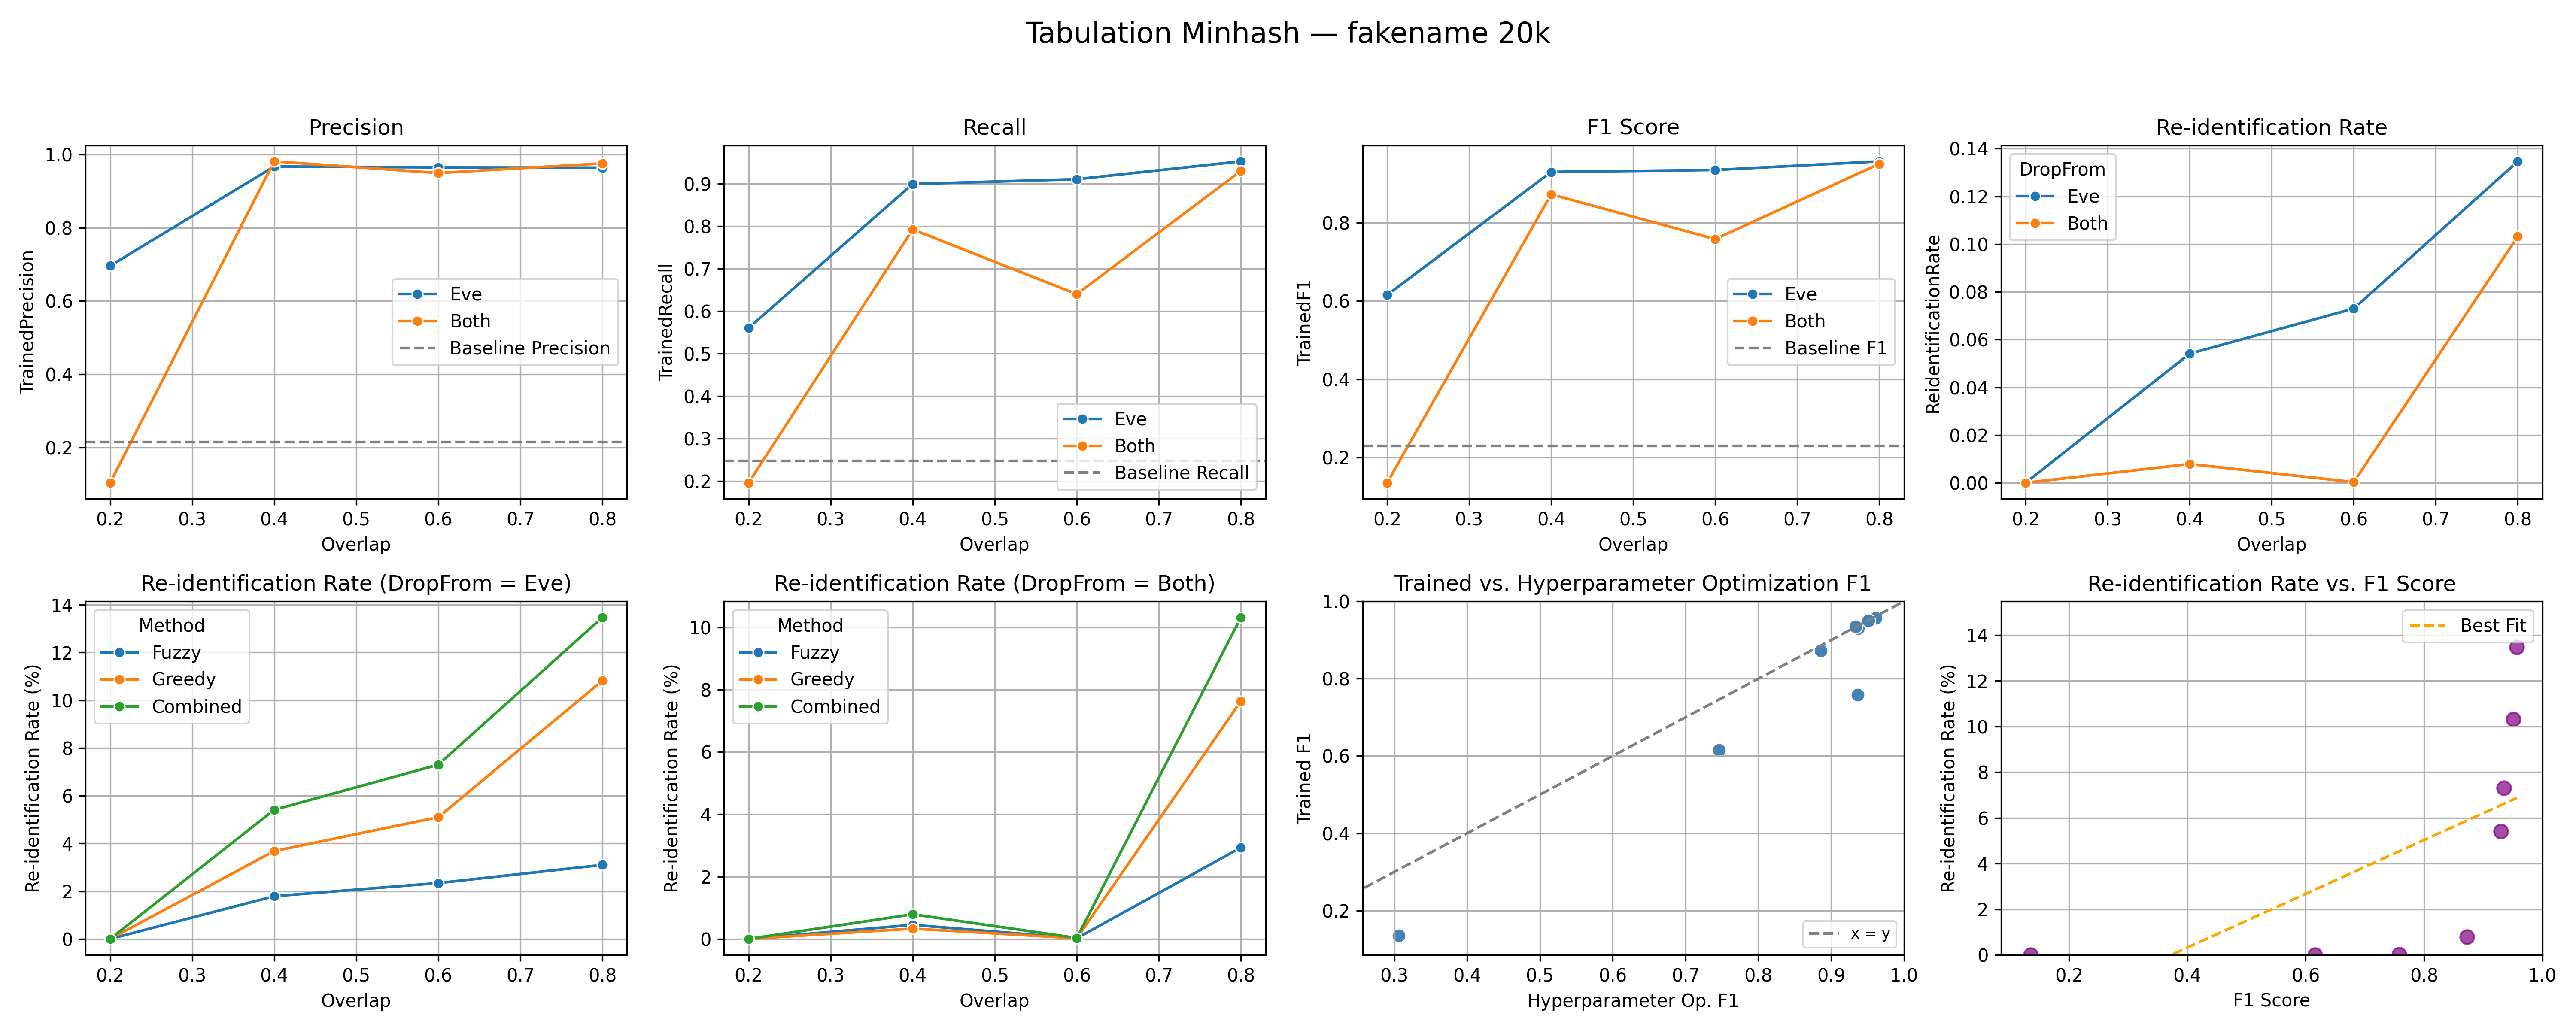
\includegraphics[width=\textwidth]{figures/TabMinHash_fakename_20k_metrics.png}
    \caption{\ac{tmh} results on the \texttt{fakename\_20k} dataset.}
    \label{fig:tabminhash_fakename20k}
\end{figure}

\begin{figure}[H]
    \centering
    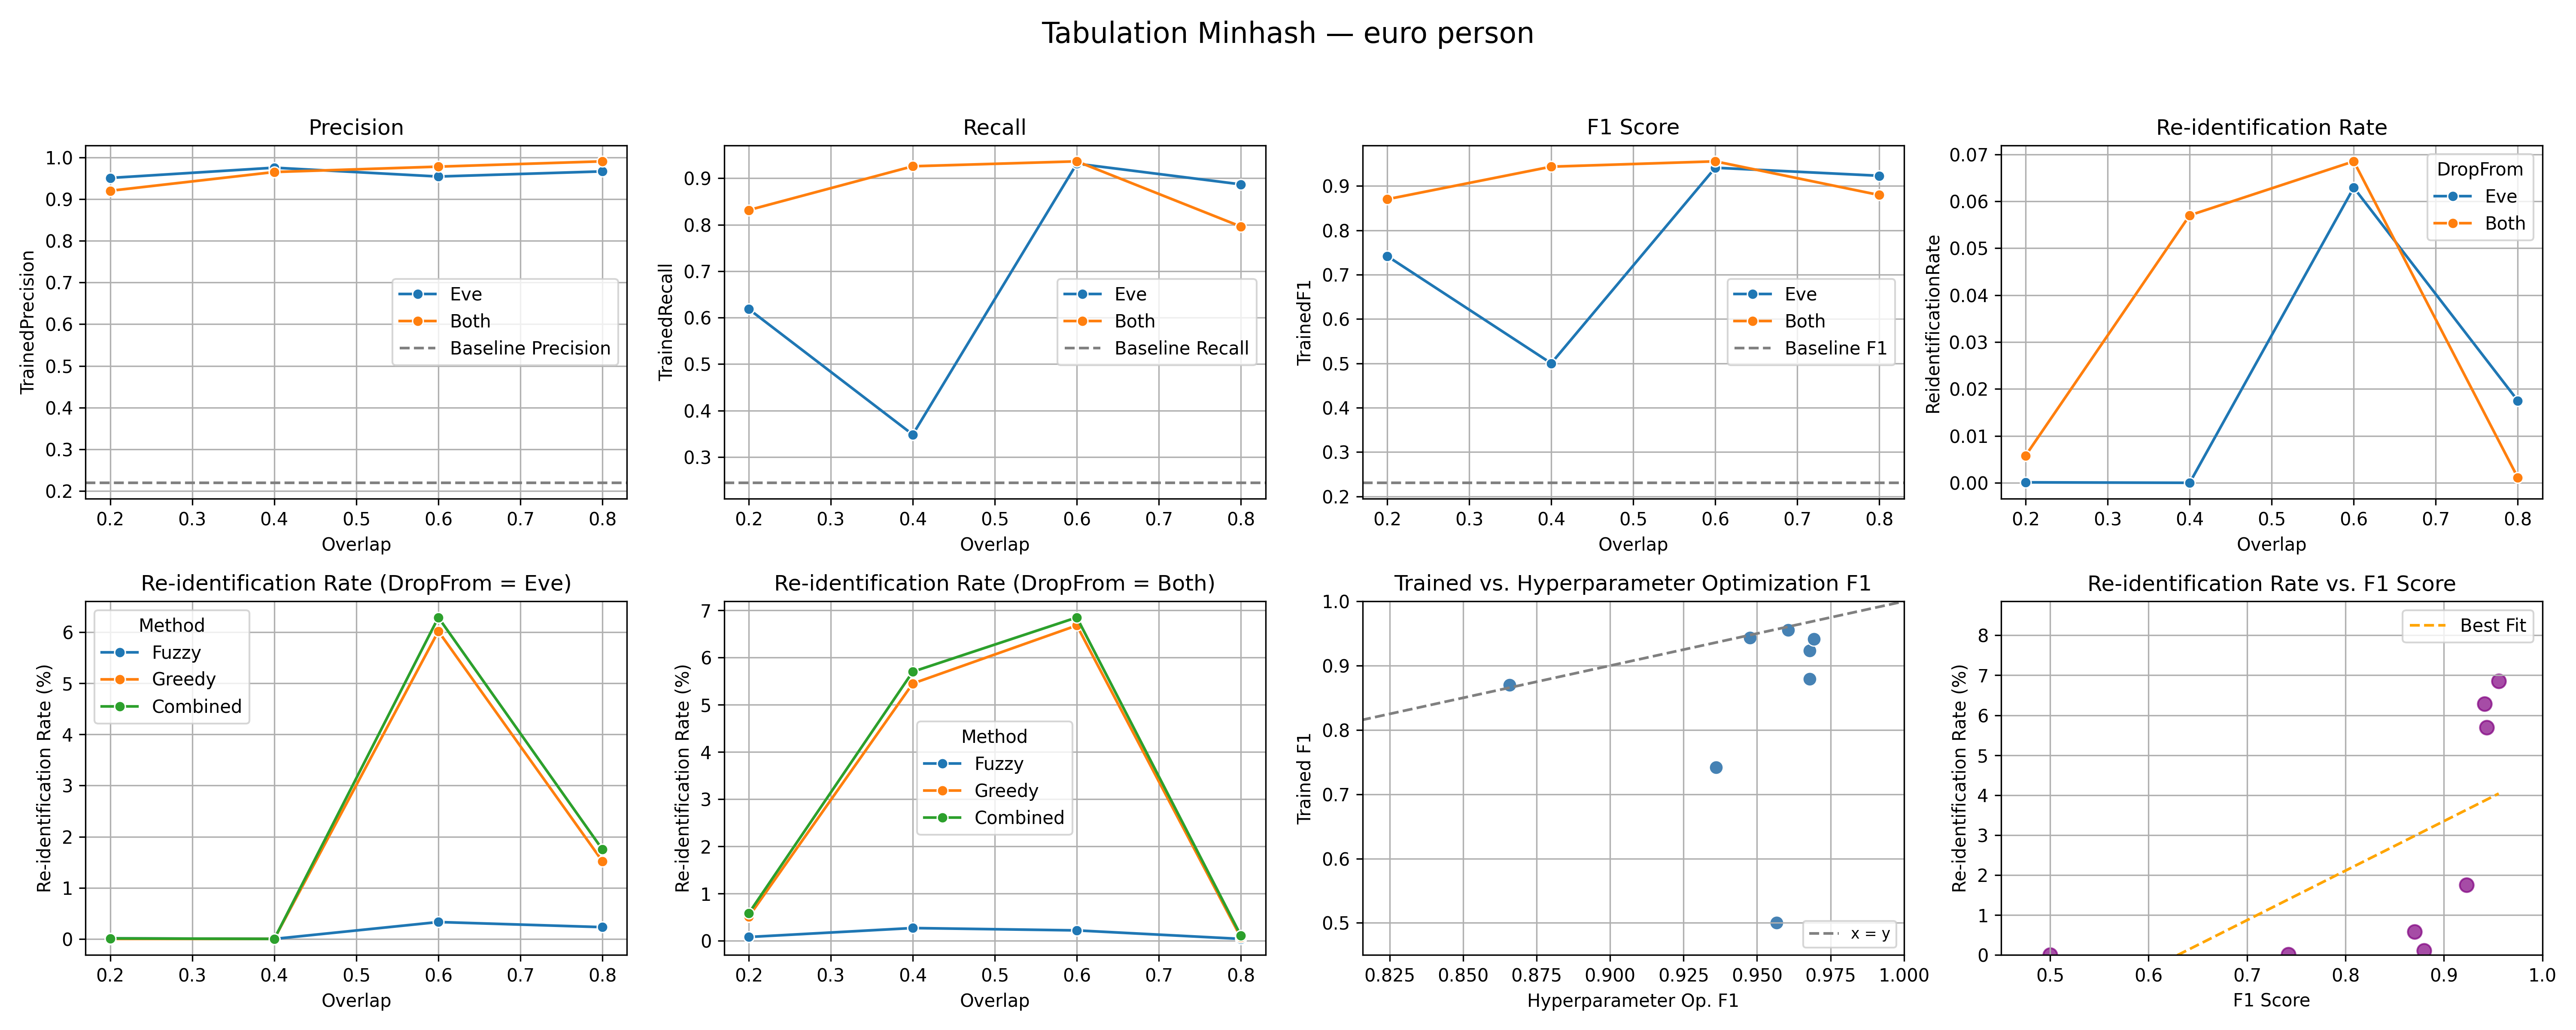
\includegraphics[width=\textwidth]{figures/TabMinHash_euro_person_metrics.png}
    \caption{\ac{tmh} results on the \texttt{euro\_person} dataset.}
    \label{fig:tabminhash_euro}
\end{figure}

\begin{figure}[H]
    \centering
    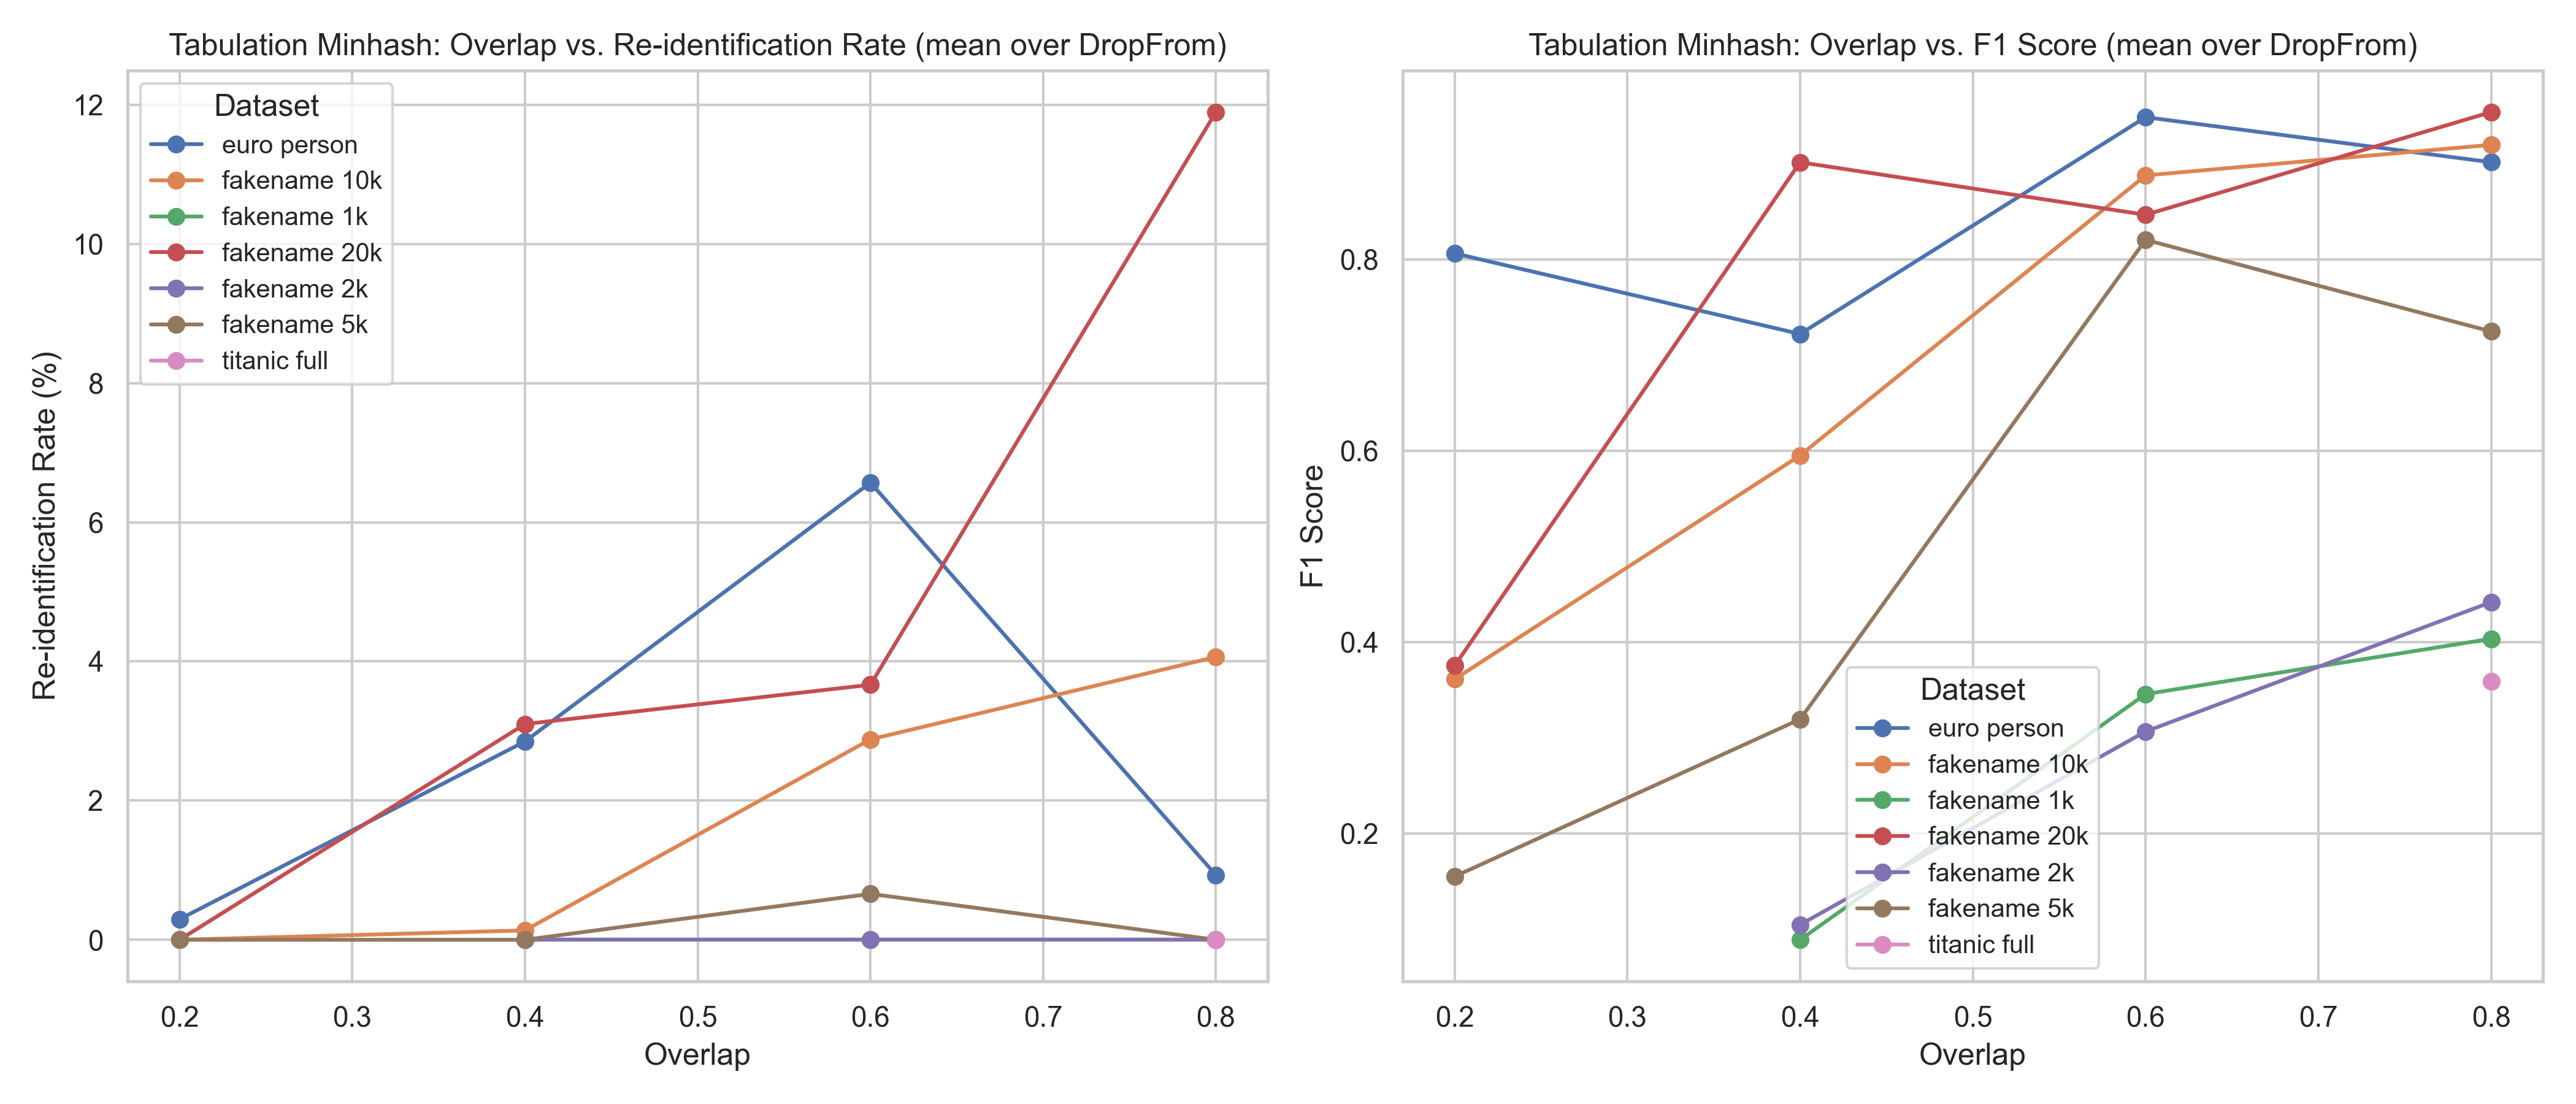
\includegraphics[width=\textwidth]{figures/TabMinHash_overlap_summary.png}
    \caption{Comparison of re-identification rates and F1 scores across all datasets with \ac{tmh} encoding as a function of overlap.}
    \label{fig:tabminhash_overlap}
\end{figure}

\begin{figure}[H]
    \centering
    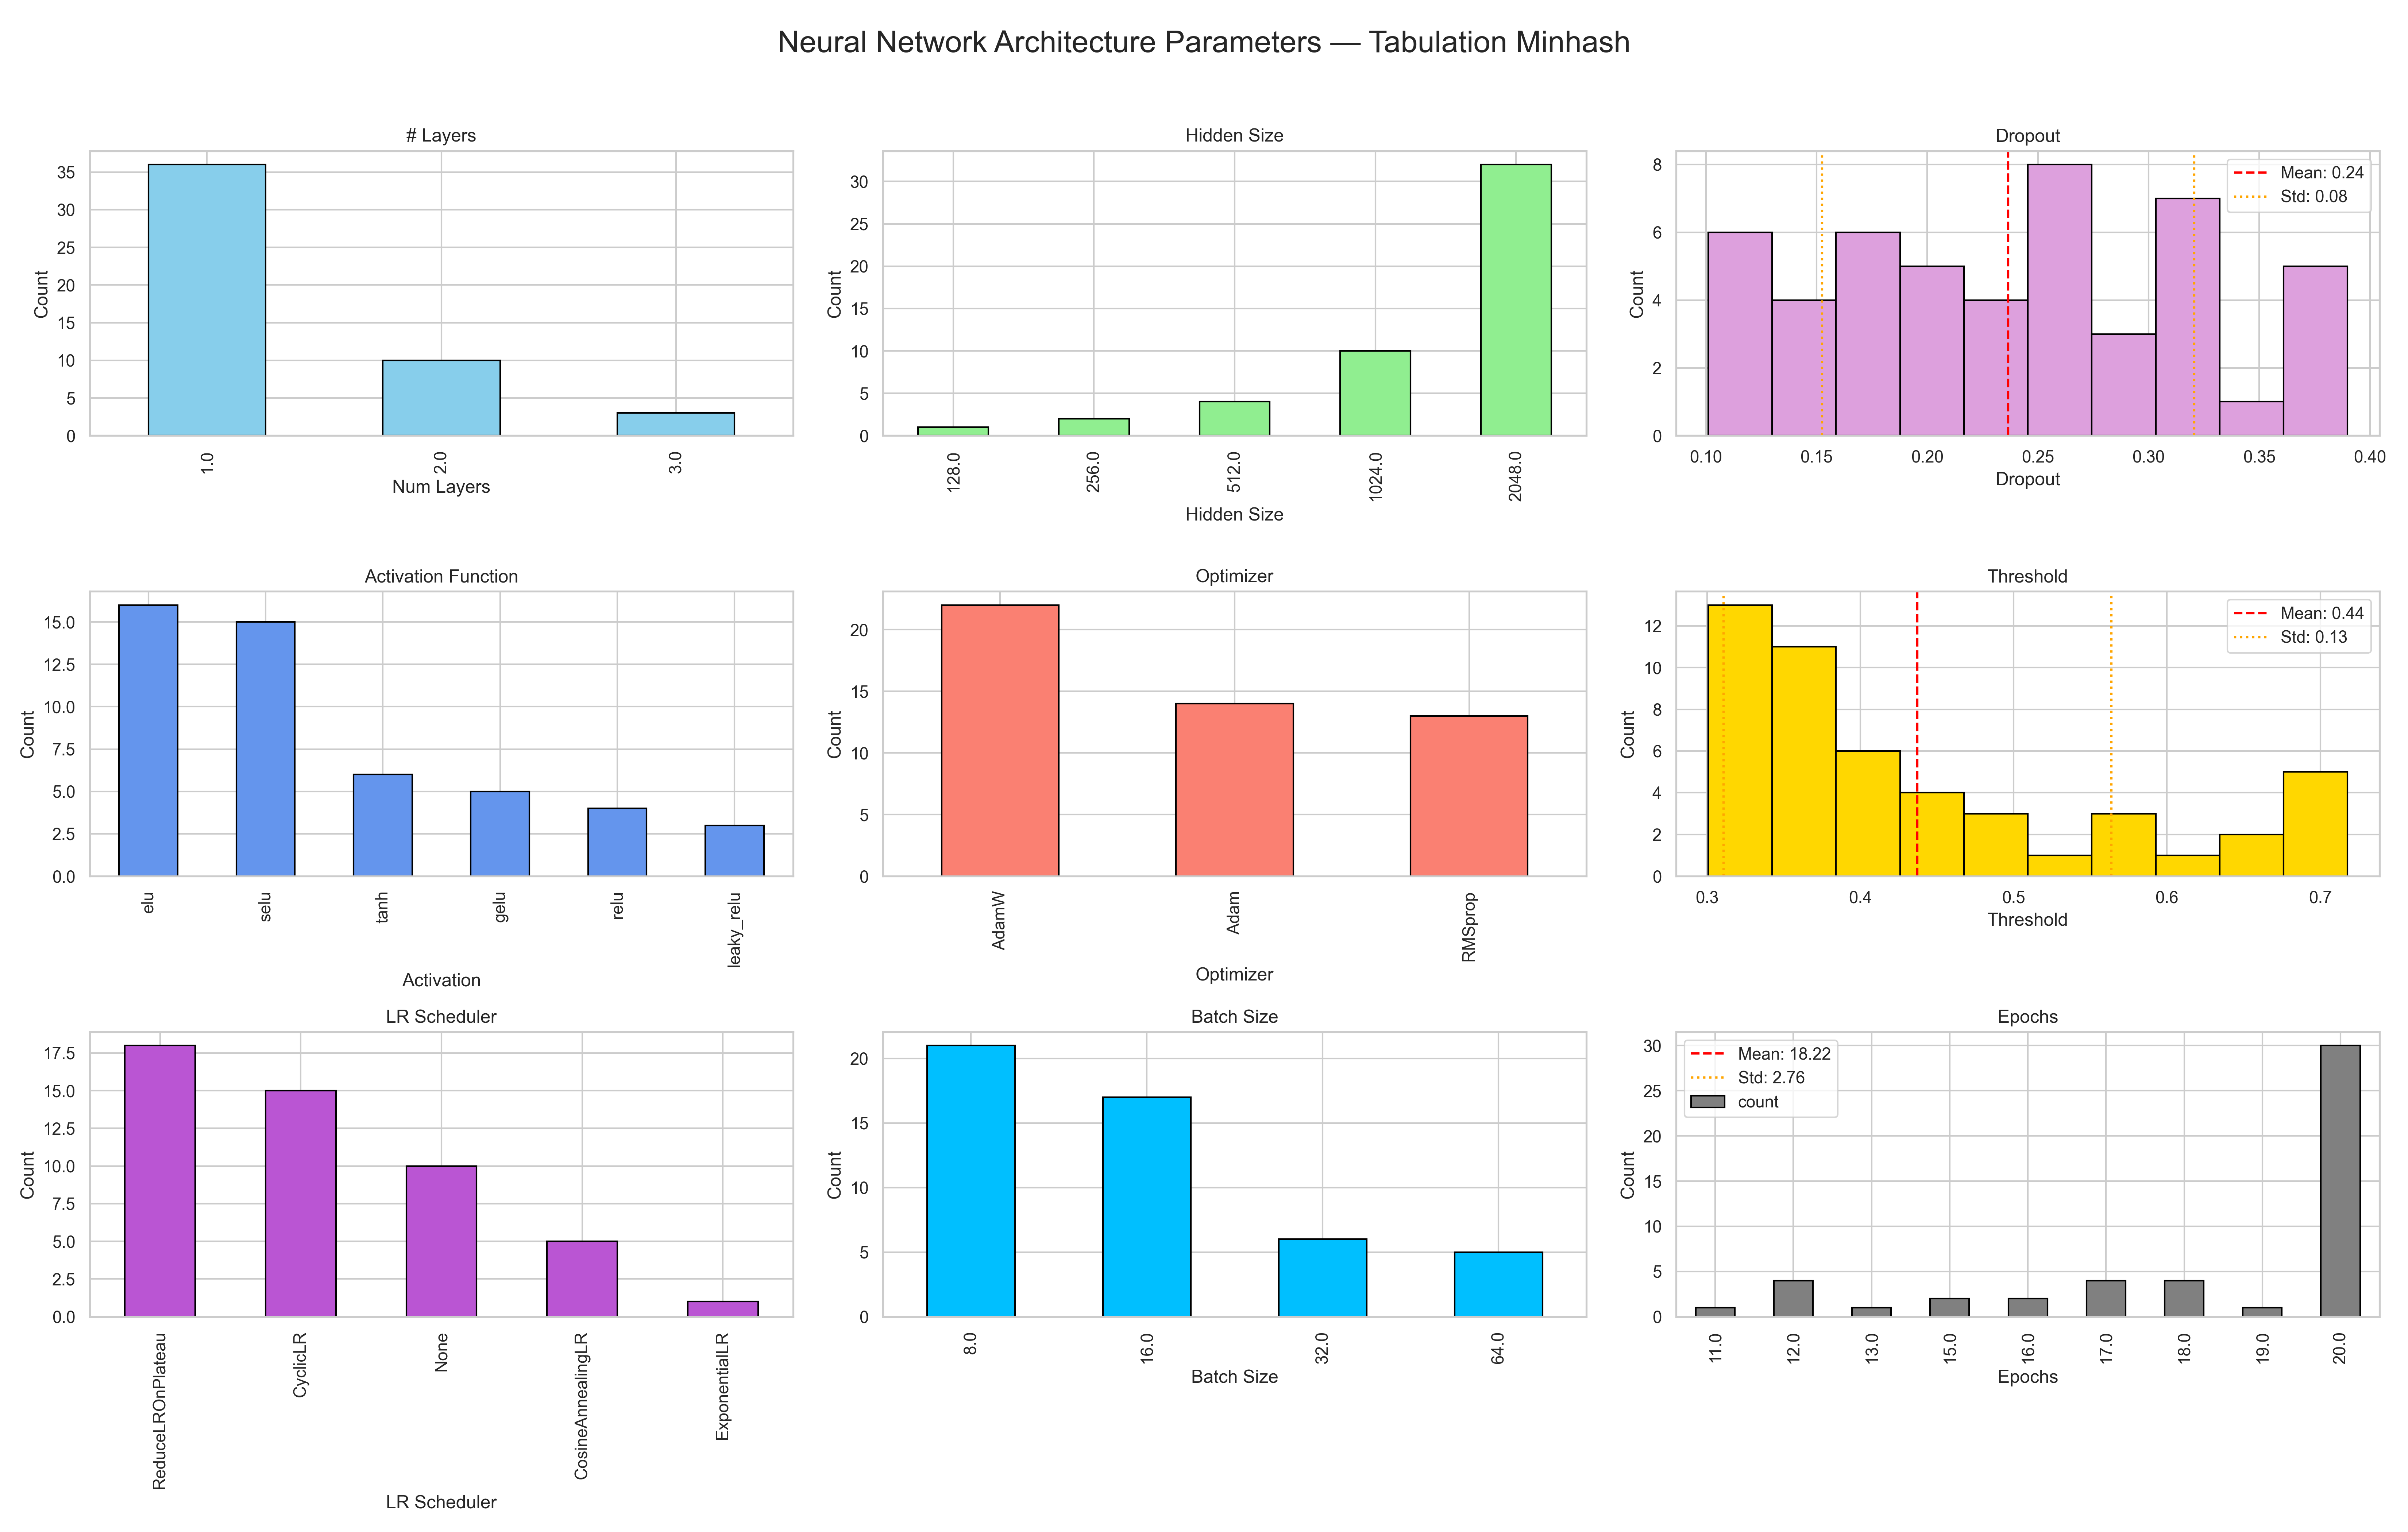
\includegraphics[width=\textwidth]{figures/TabMinHash_architecture.png}
    \caption{Distribution of selected neural network architecture parameters during hyperparameter optimization for the \ac{tmh} encoding.}
    \label{fig:tabminhash_architecture}
\end{figure}

\clearpage

\section{\ac{tsh}: \ac{dea} Results} \label{sec:twostep_results}

\begin{figure}[H]
    \centering
    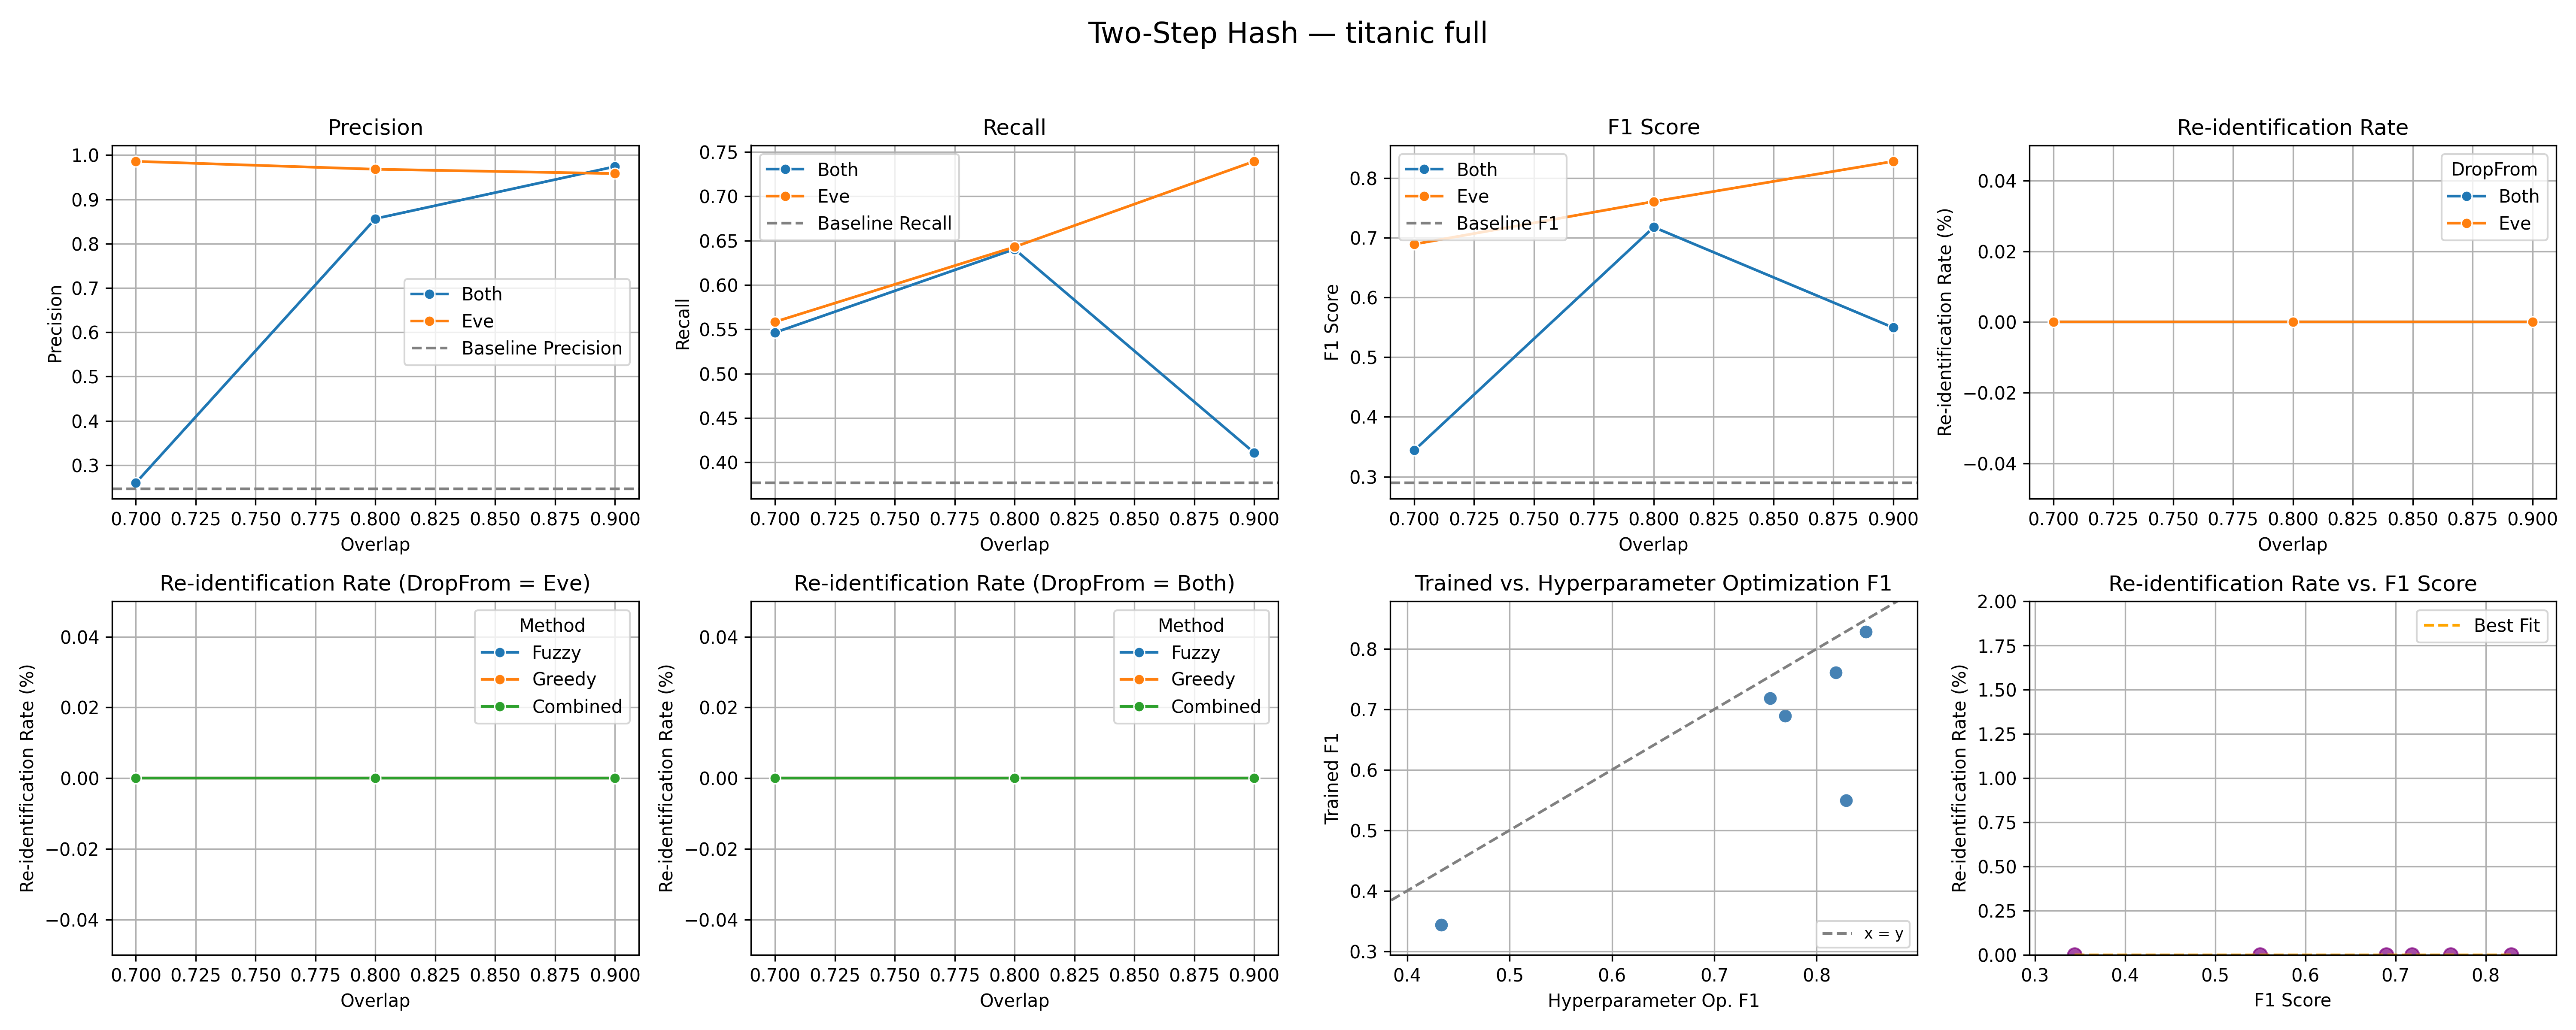
\includegraphics[width=\textwidth]{figures/TwoStepHash_titanic_full_metrics.png}
    \caption{\ac{tsh} results on the \texttt{titanic\_full} dataset.}
    \label{fig:twostep_titanic}
\end{figure}

\begin{figure}[H]
    \centering
    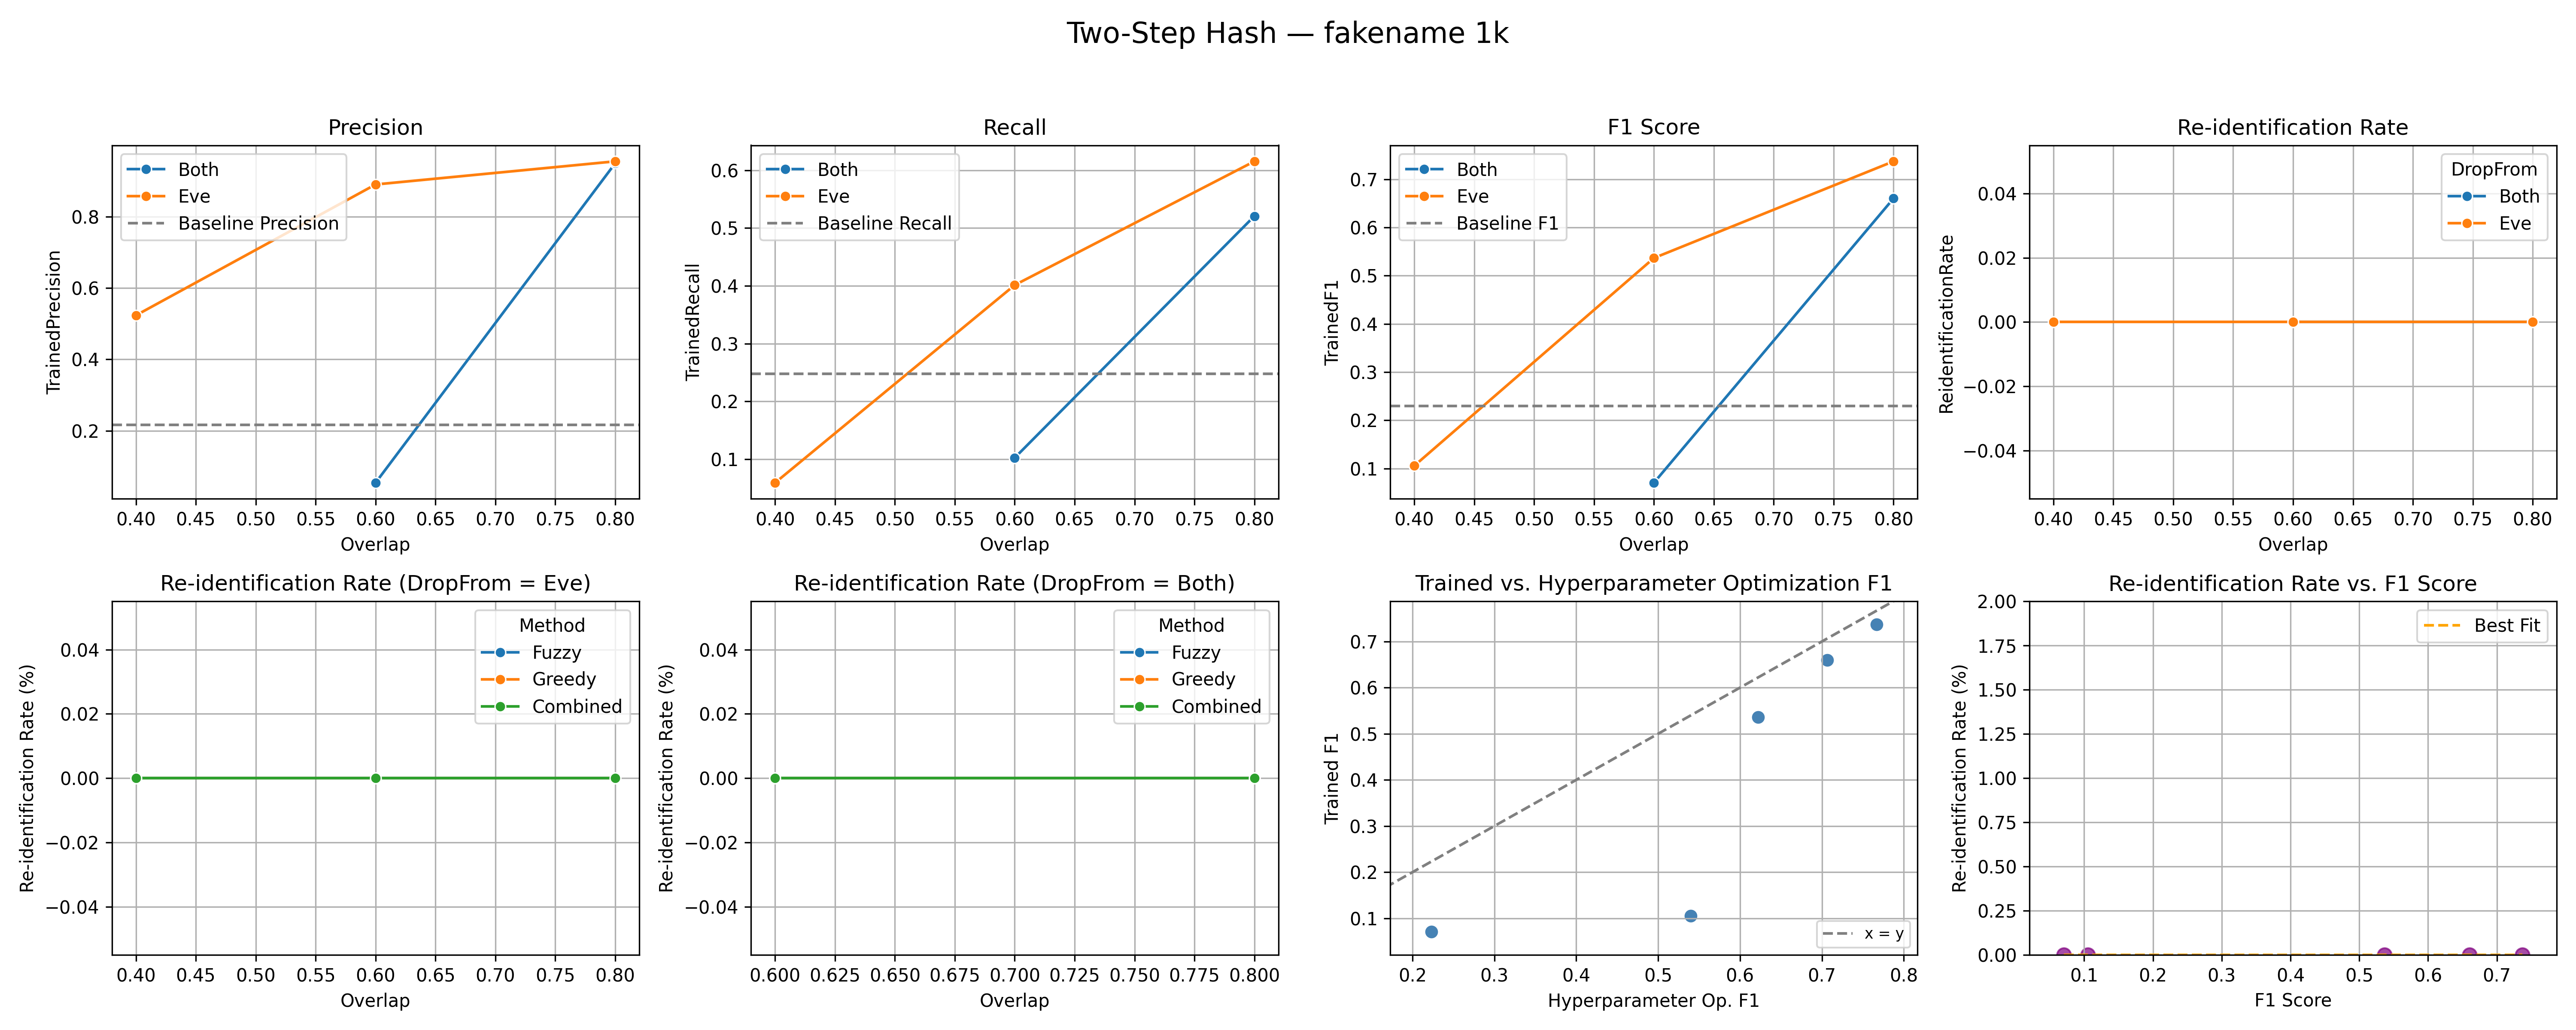
\includegraphics[width=\textwidth]{figures/TwoStepHash_fakename_1k_metrics.png}
    \caption{\ac{tsh} results on the \texttt{fakename\_1k} dataset.}
    \label{fig:twostep_fakename1k}
\end{figure}

\begin{figure}[H]
    \centering
    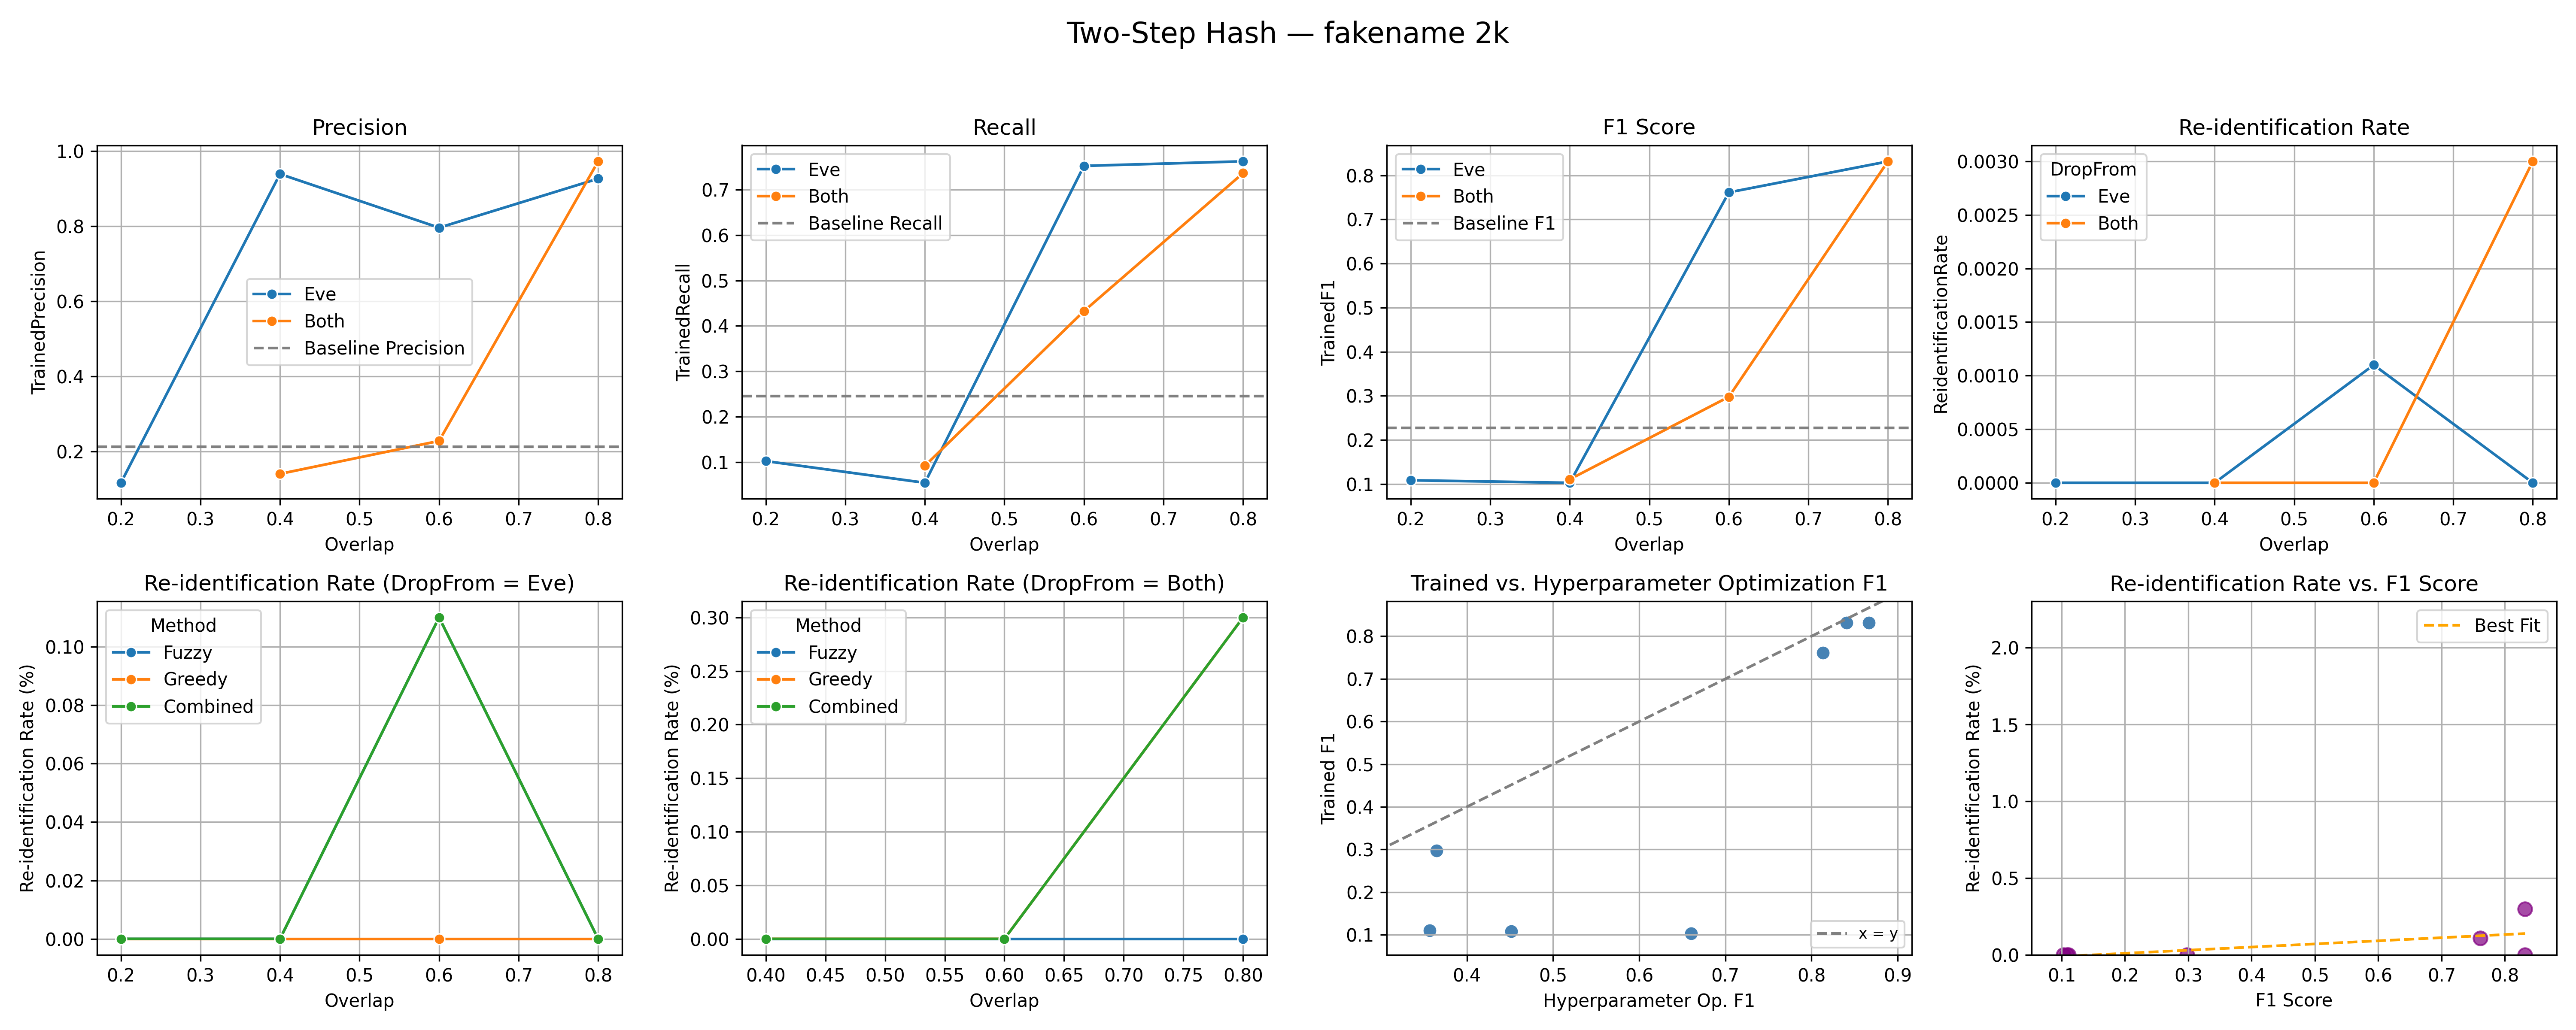
\includegraphics[width=\textwidth]{figures/TwoStepHash_fakename_2k_metrics.png}
    \caption{\ac{tsh} results on the \texttt{fakename\_2k} dataset.}
    \label{fig:twostep_fakename2k}
\end{figure}

\begin{figure}[H]
    \centering
    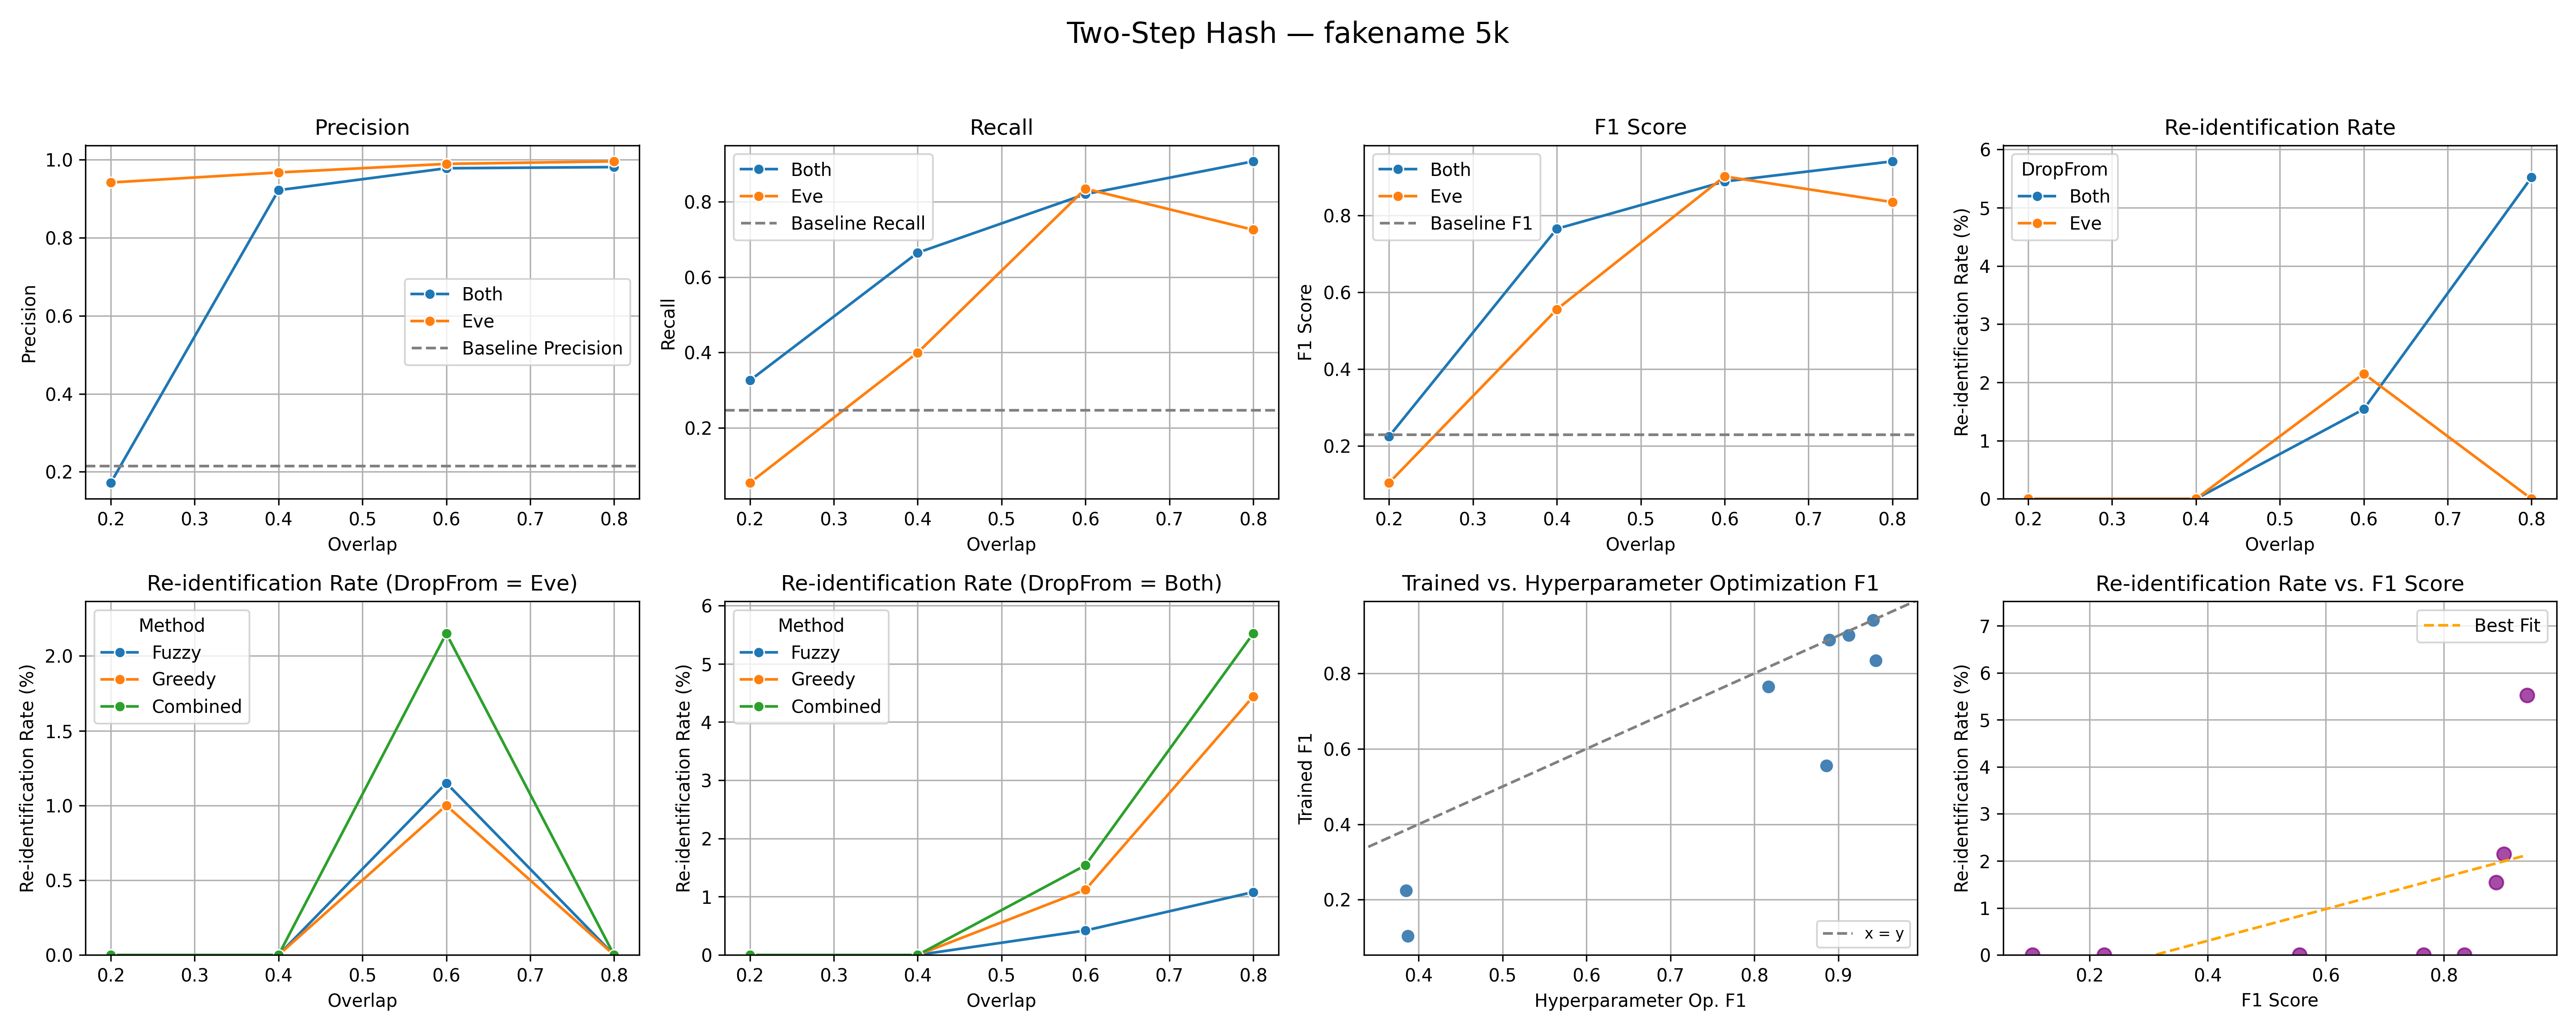
\includegraphics[width=\textwidth]{figures/TwoStepHash_fakename_5k_metrics.png}
    \caption{\ac{tsh} results on the \texttt{fakename\_5k} dataset.}
    \label{fig:twostep_fakename5k}
\end{figure}

\begin{figure}[H]
    \centering
    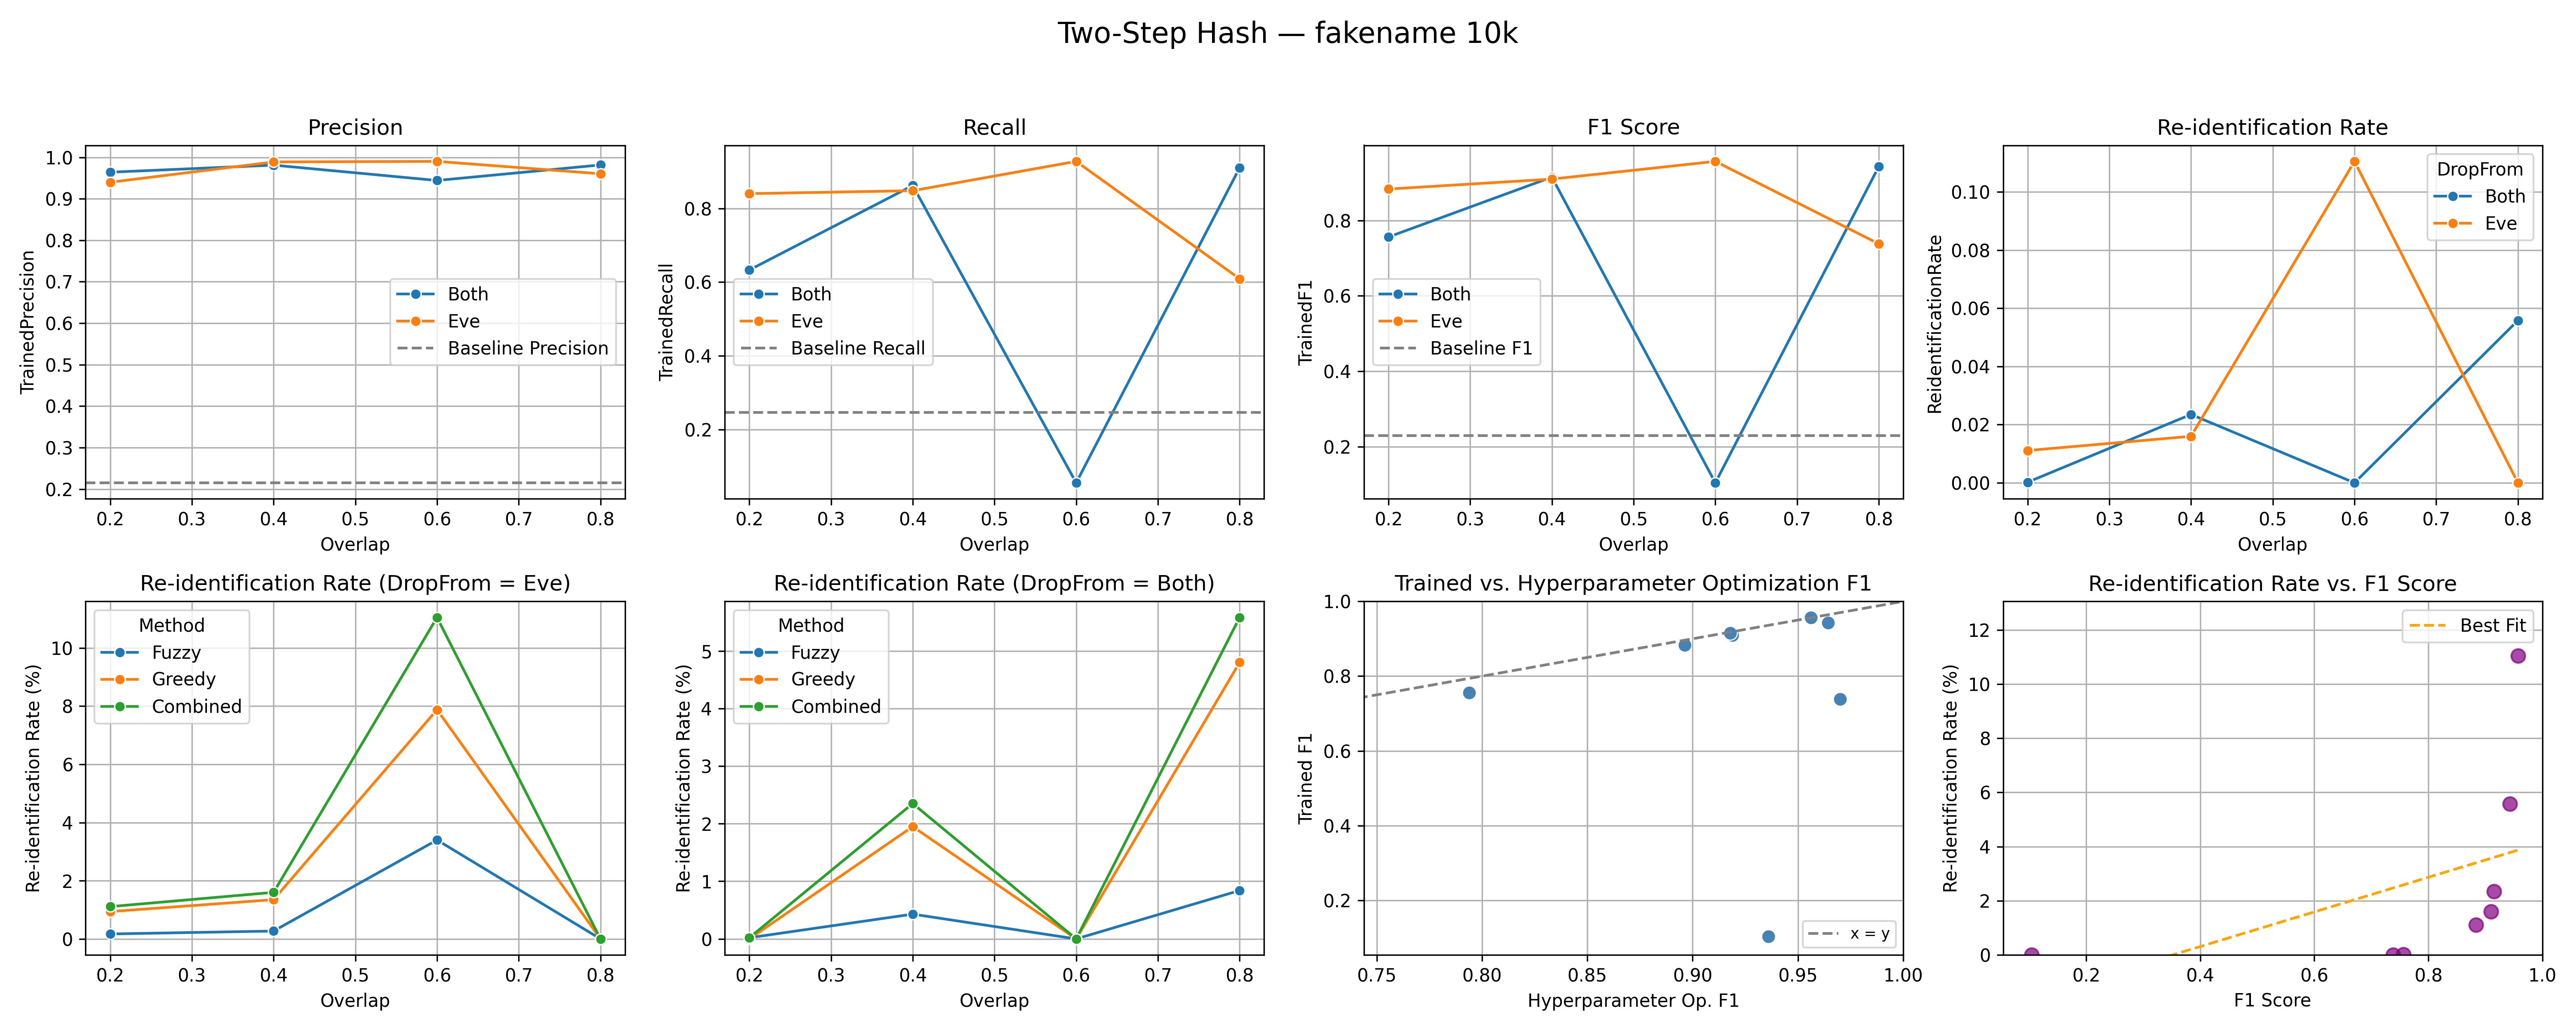
\includegraphics[width=\textwidth]{figures/TwoStepHash_fakename_10k_metrics.png}
    \caption{\ac{tsh} results on the \texttt{fakename\_10k} dataset.}
    \label{fig:twostep_fakename10k}
\end{figure}

\begin{figure}[H]
    \centering
    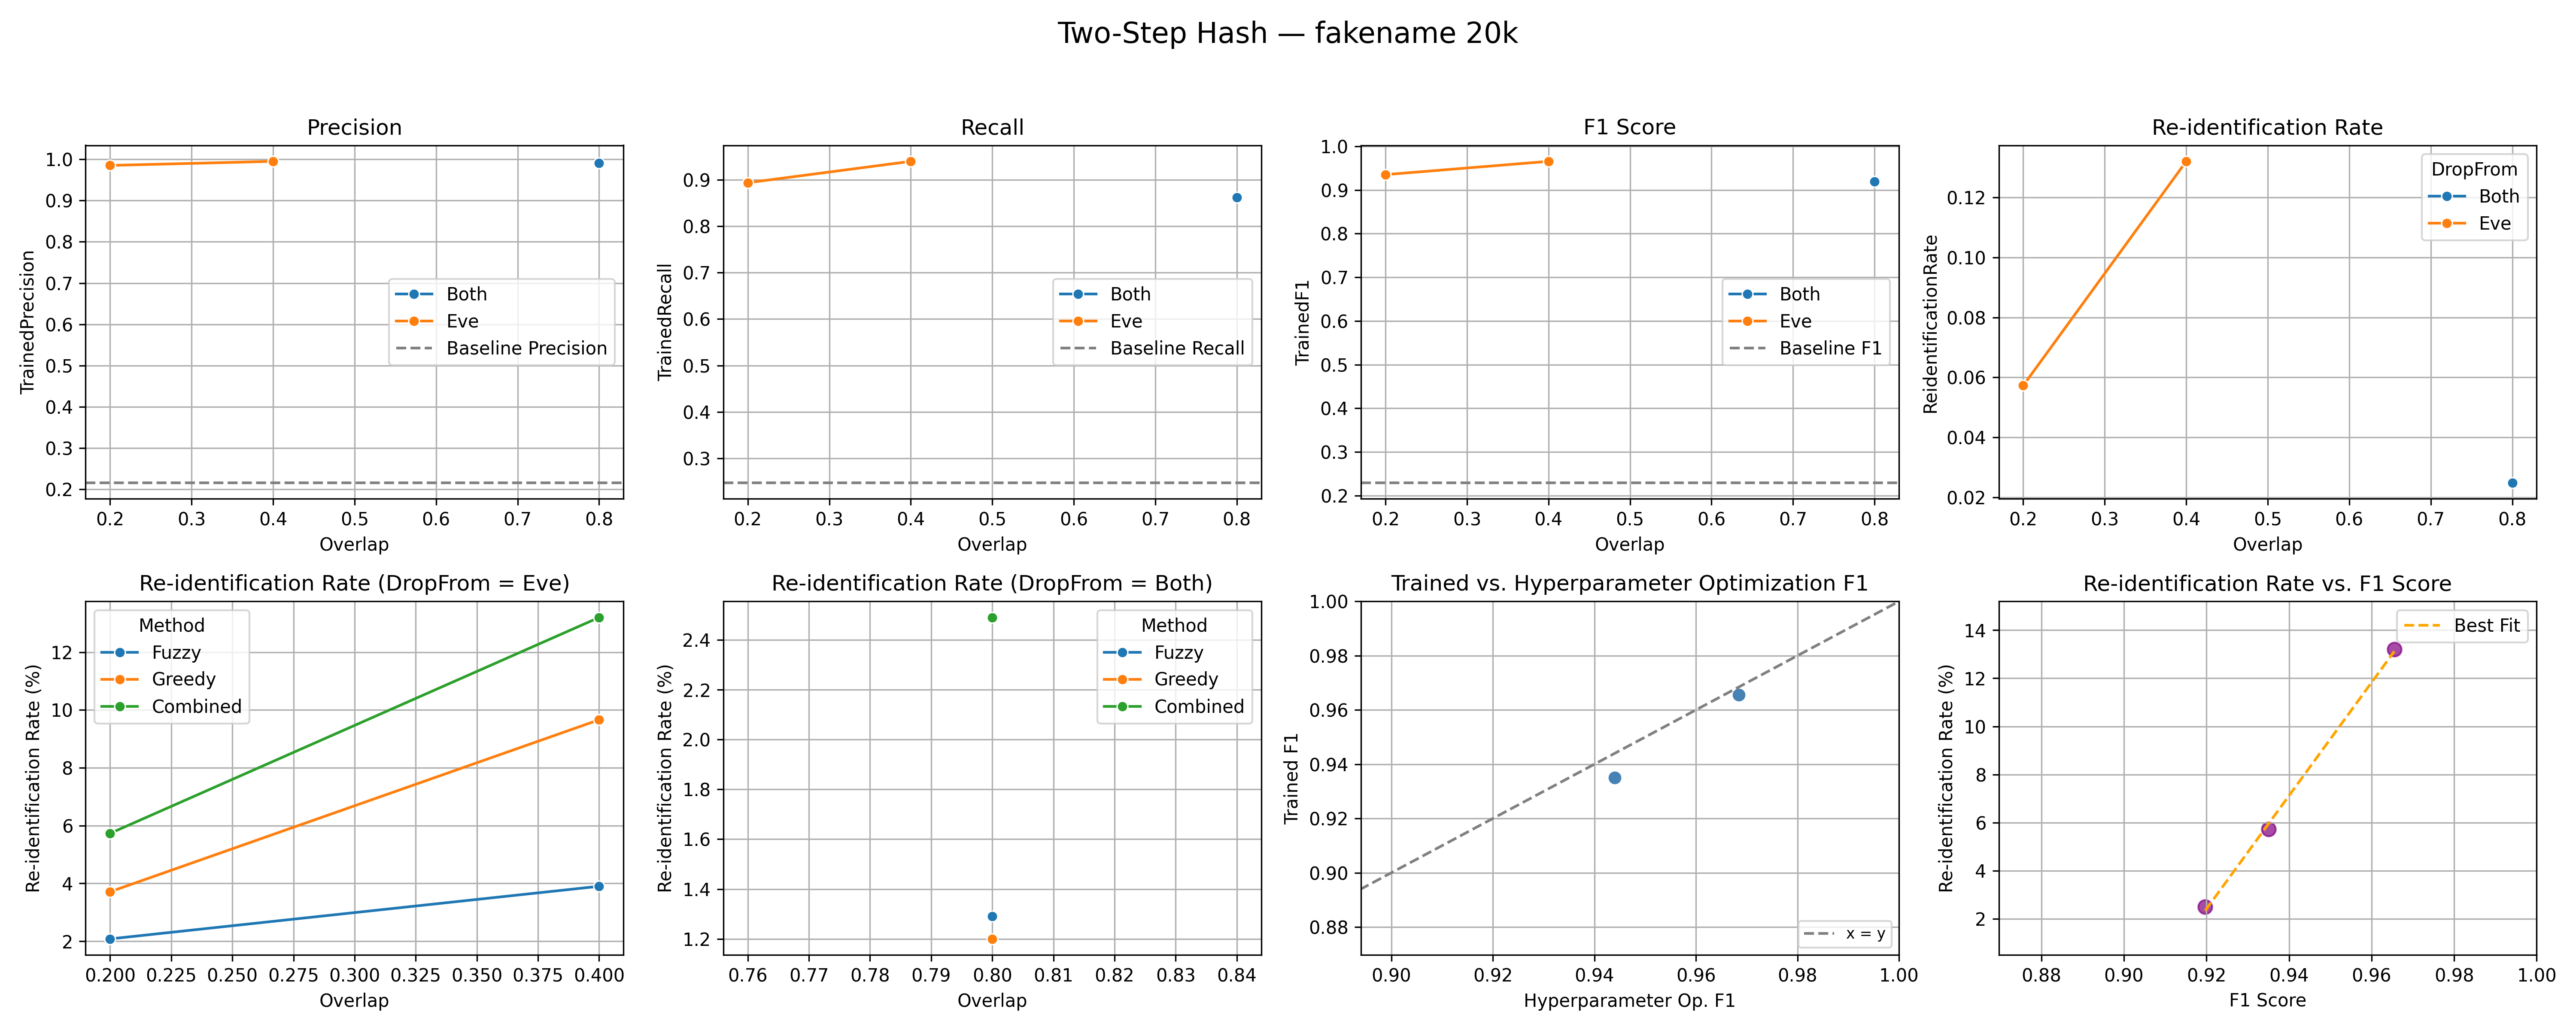
\includegraphics[width=\textwidth]{figures/TwoStepHash_fakename_20k_metrics.png}
    \caption{\ac{tsh} results on the \texttt{fakename\_20k} dataset.}
    \label{fig:twostep_fakename20k}
\end{figure}

\begin{figure}[H]
    \centering
    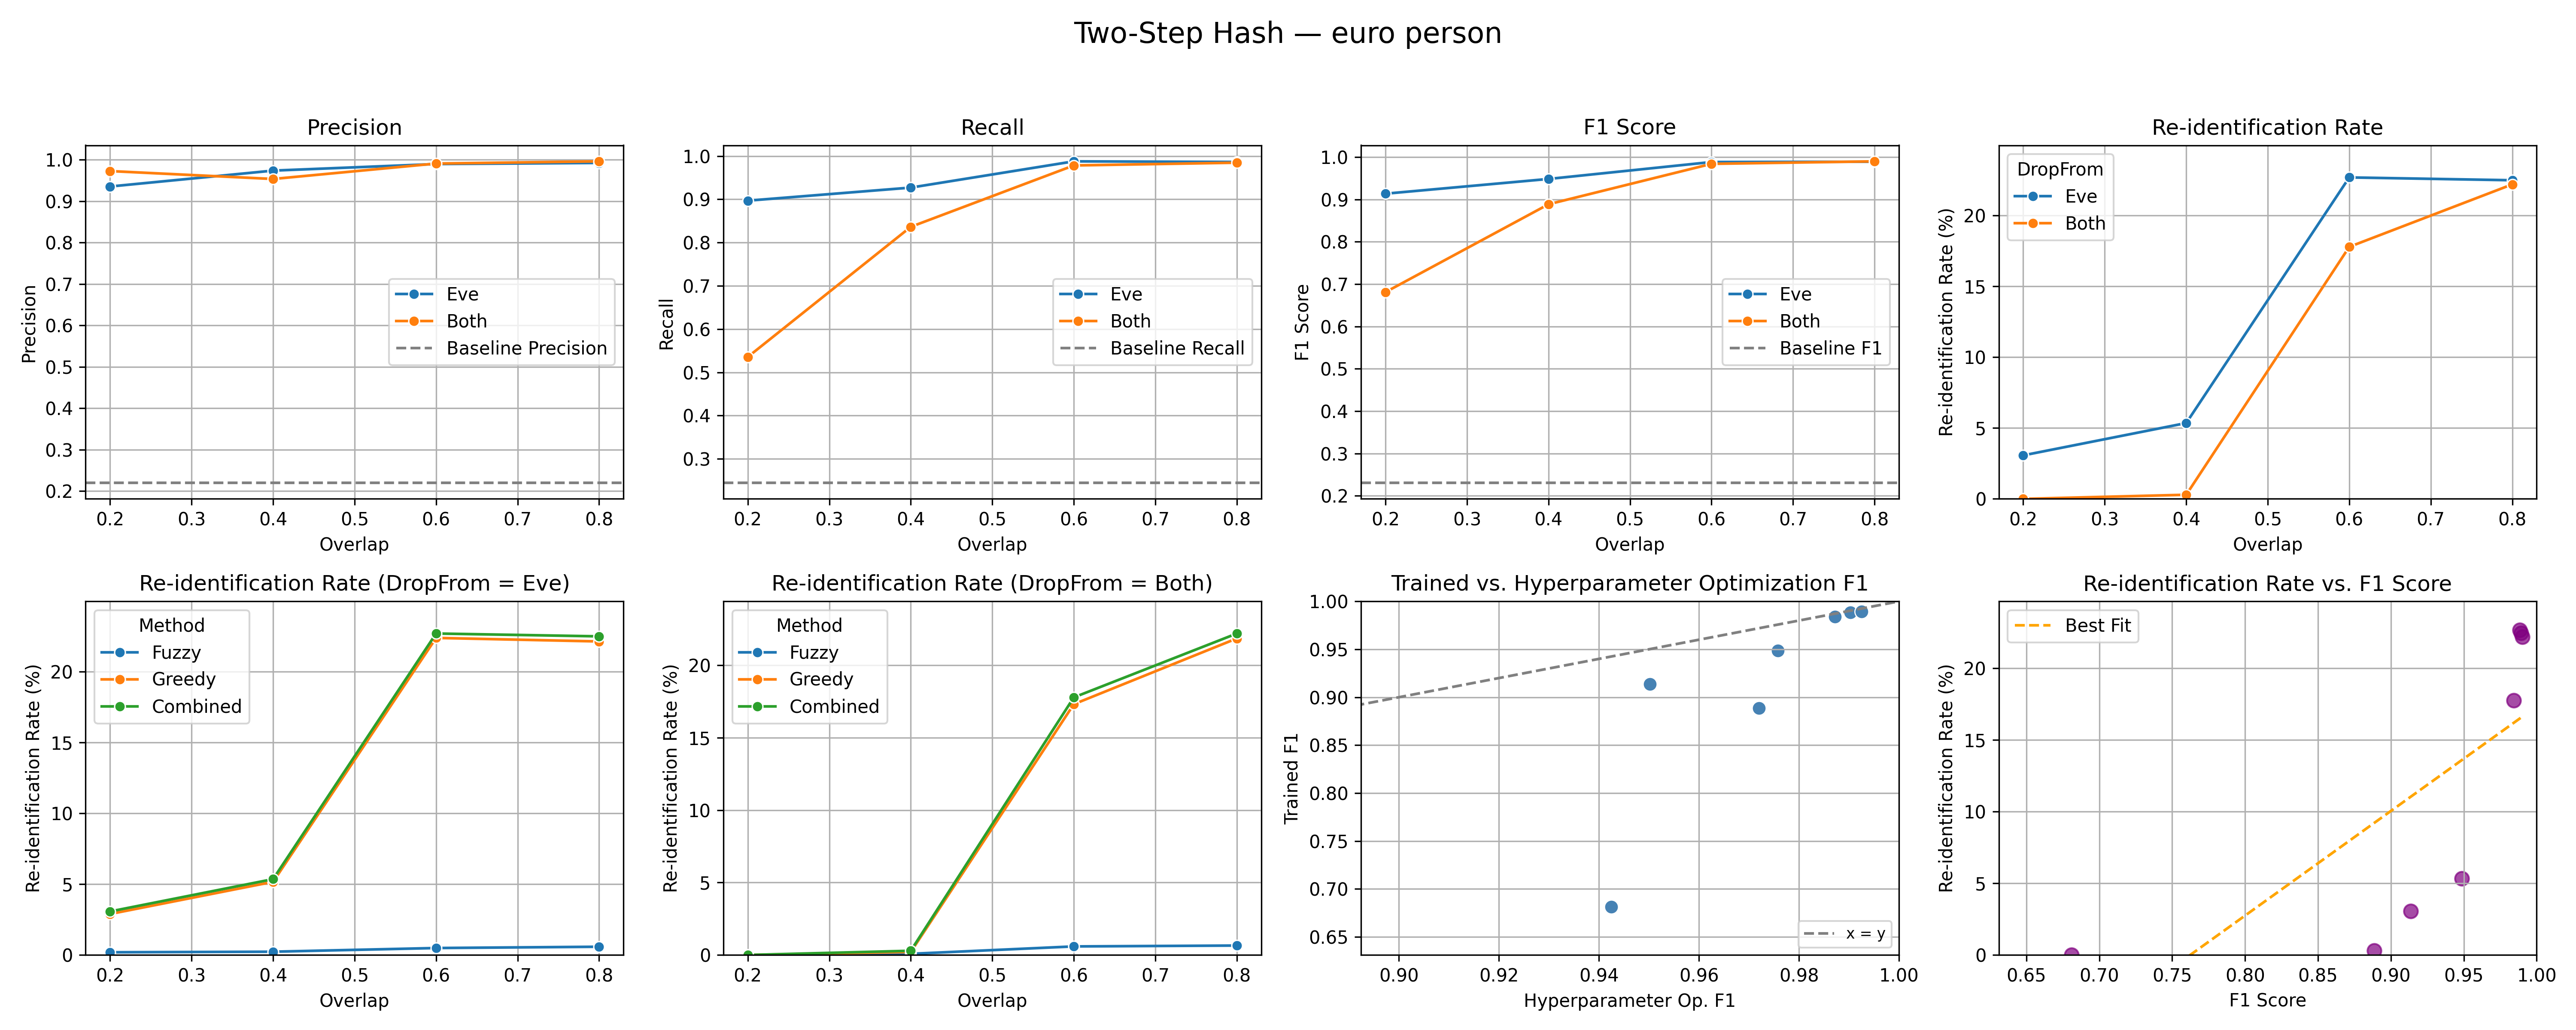
\includegraphics[width=\textwidth]{figures/TwoStepHash_euro_person_metrics.png}
    \caption{\ac{tsh} results on the \texttt{euro\_person} dataset.}
    \label{fig:twostep_euro}
\end{figure}

\begin{figure}[H]
    \centering
    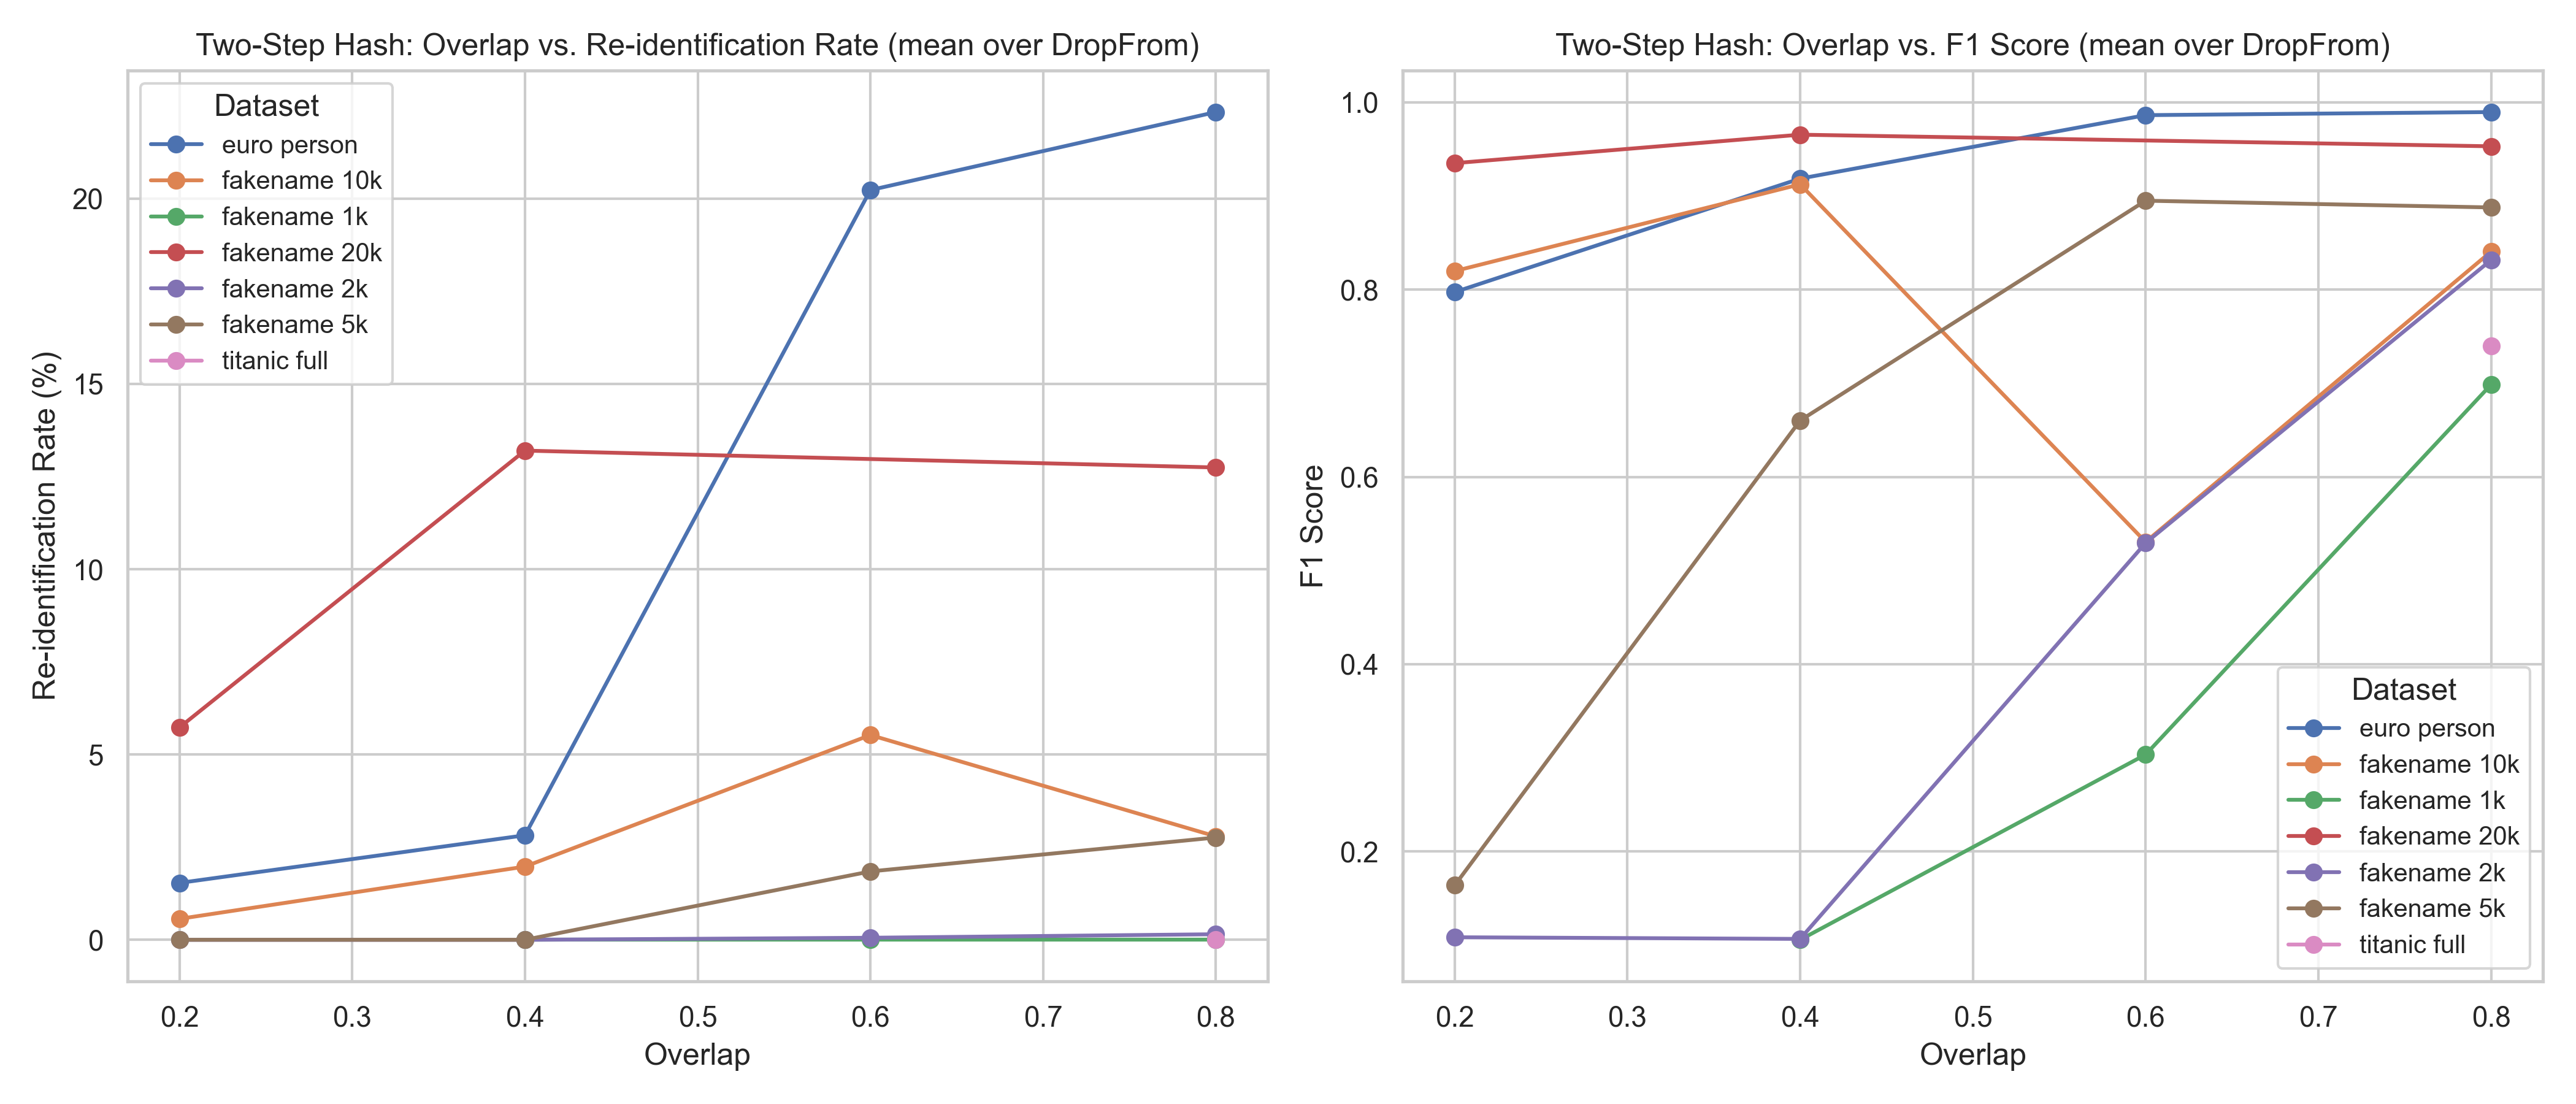
\includegraphics[width=\textwidth]{figures/TwoStepHash_overlap_summary.png}
    \caption{Comparison of re-identification rates and F1 scores across all datasets with \ac{tsh} encoding as a function of overlap.}
    \label{fig:twostep_overlap}
\end{figure}

\begin{figure}[H]
    \centering
    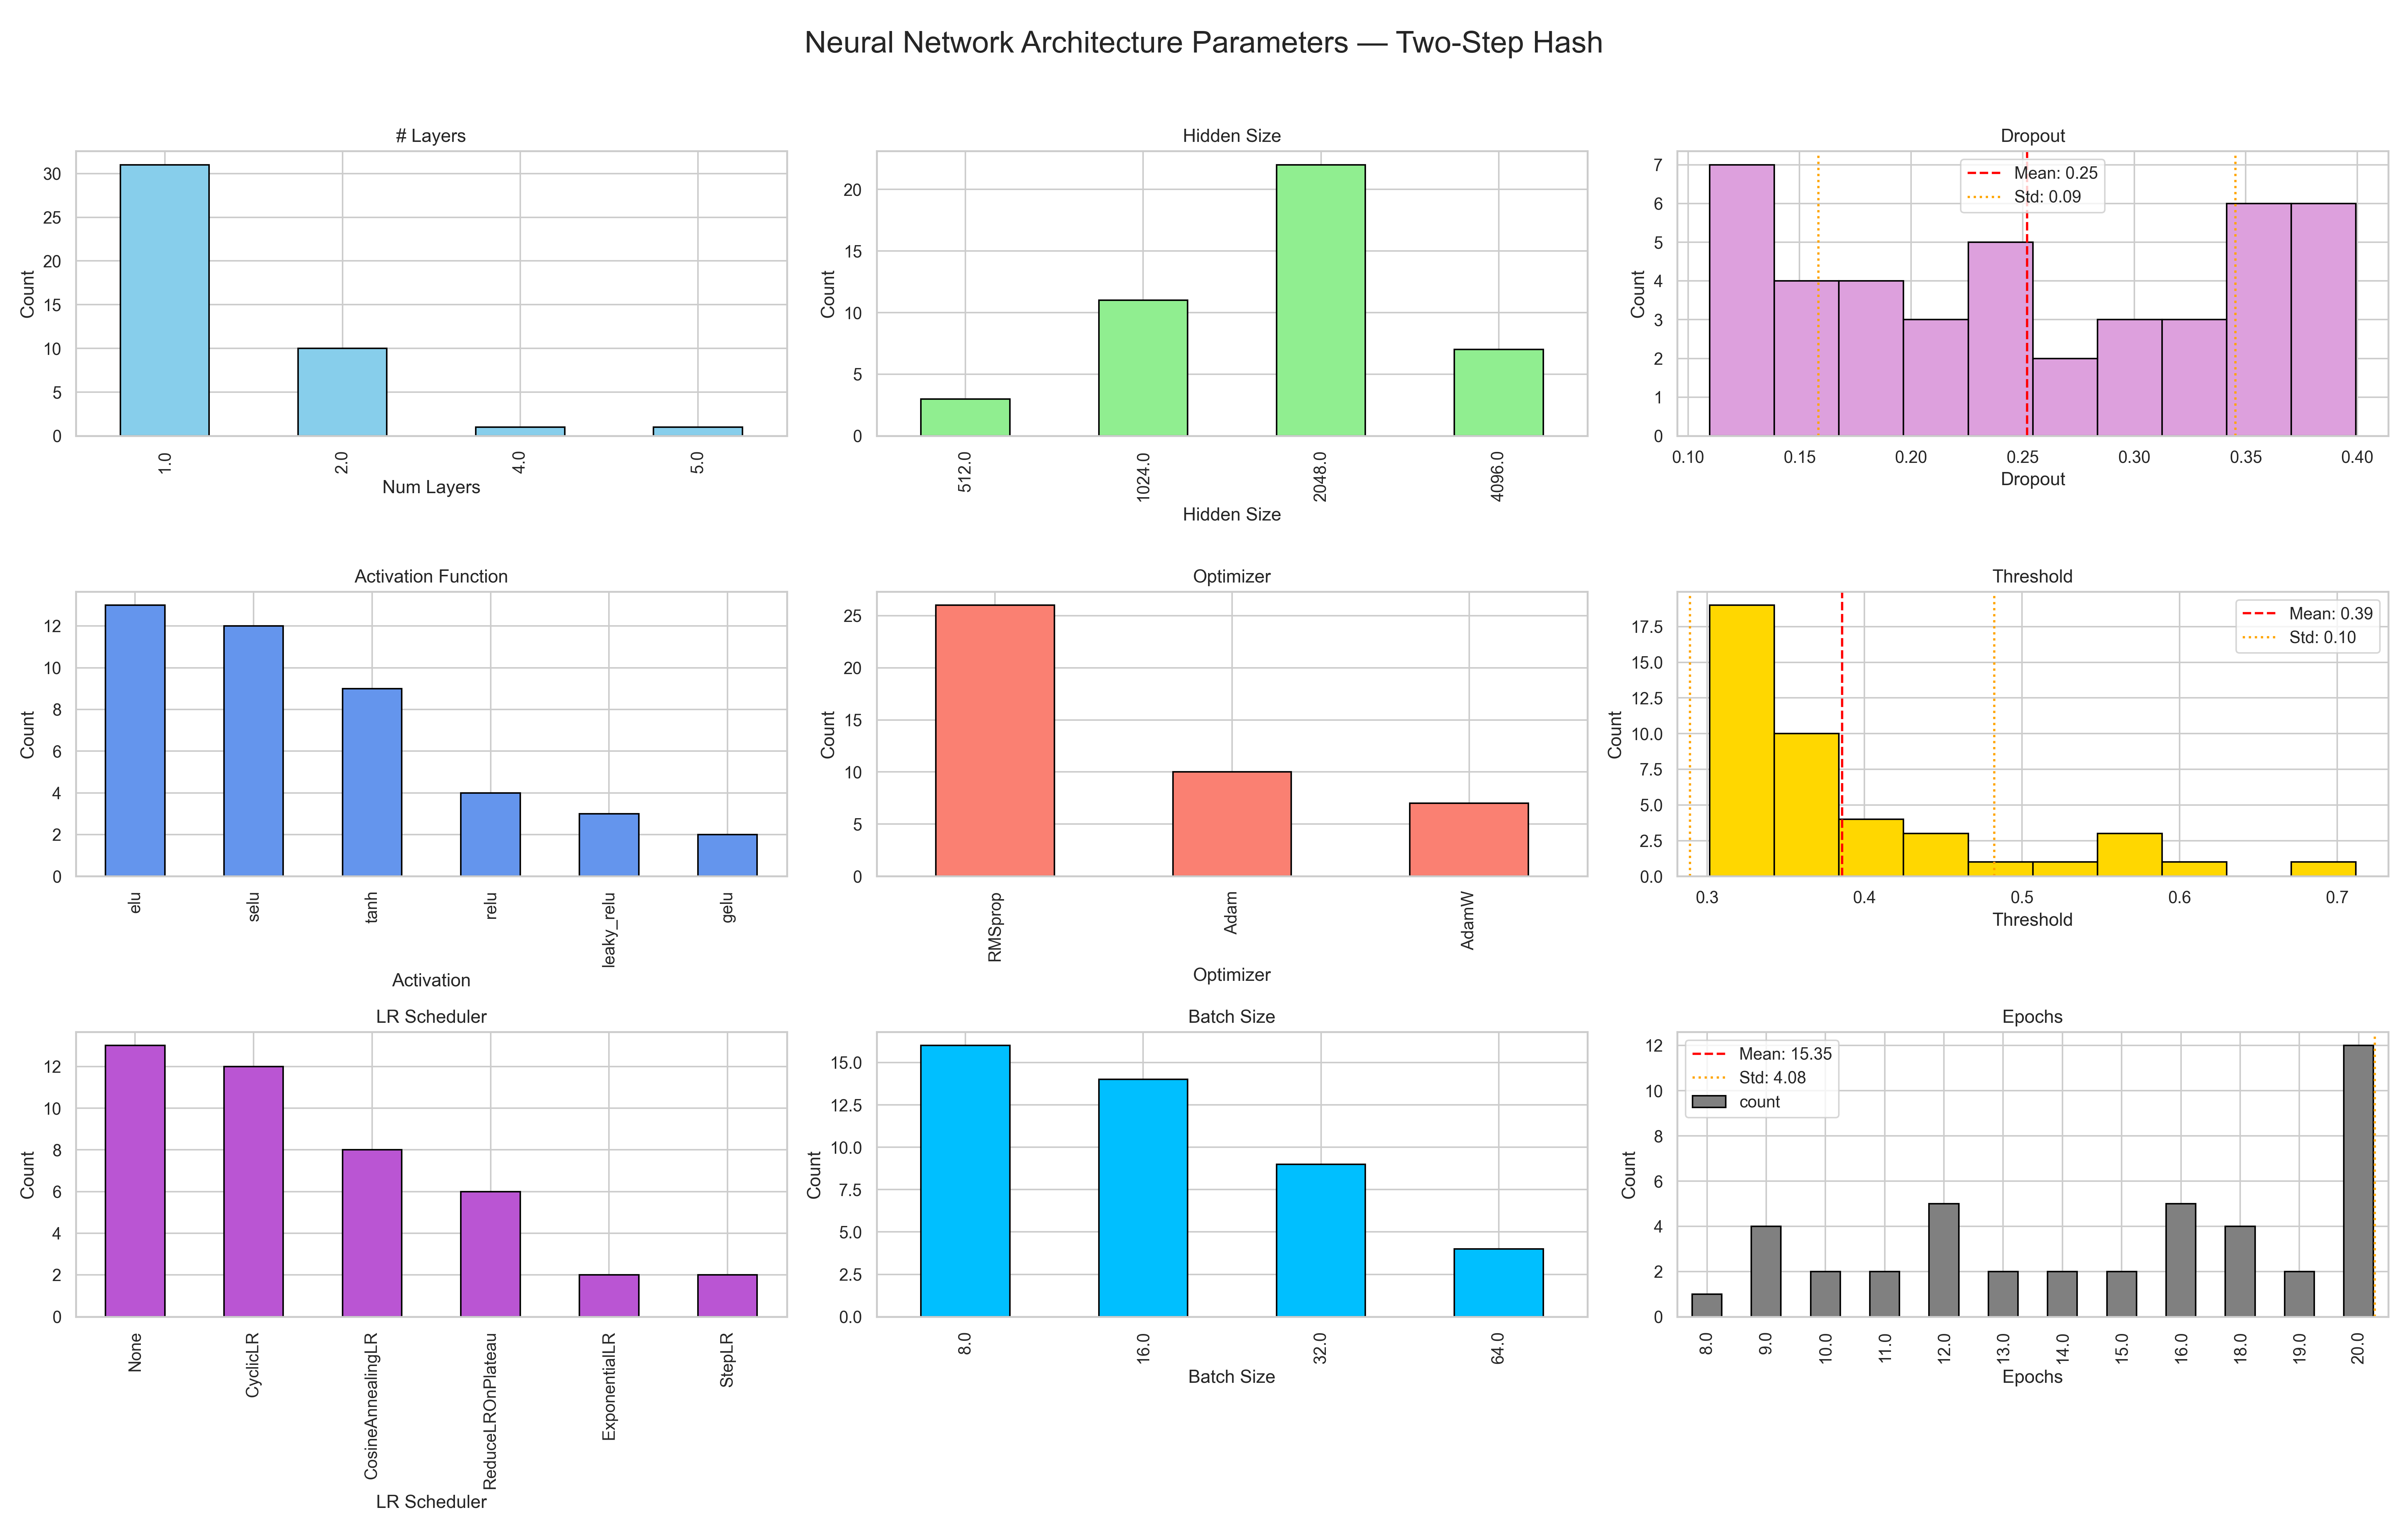
\includegraphics[width=\textwidth]{figures/TwoStepHash_architecture.png}
    \caption{Distribution of selected neural network architecture parameters during hyperparameter optimization for the \ac{tsh} encoding.}
    \label{fig:twostep_architecture}
\end{figure}

\clearpage

\section{\ac{bf}: \ac{dea} Results} \label{sec:bloomfilter_results}

\begin{figure}[H]
    \centering
    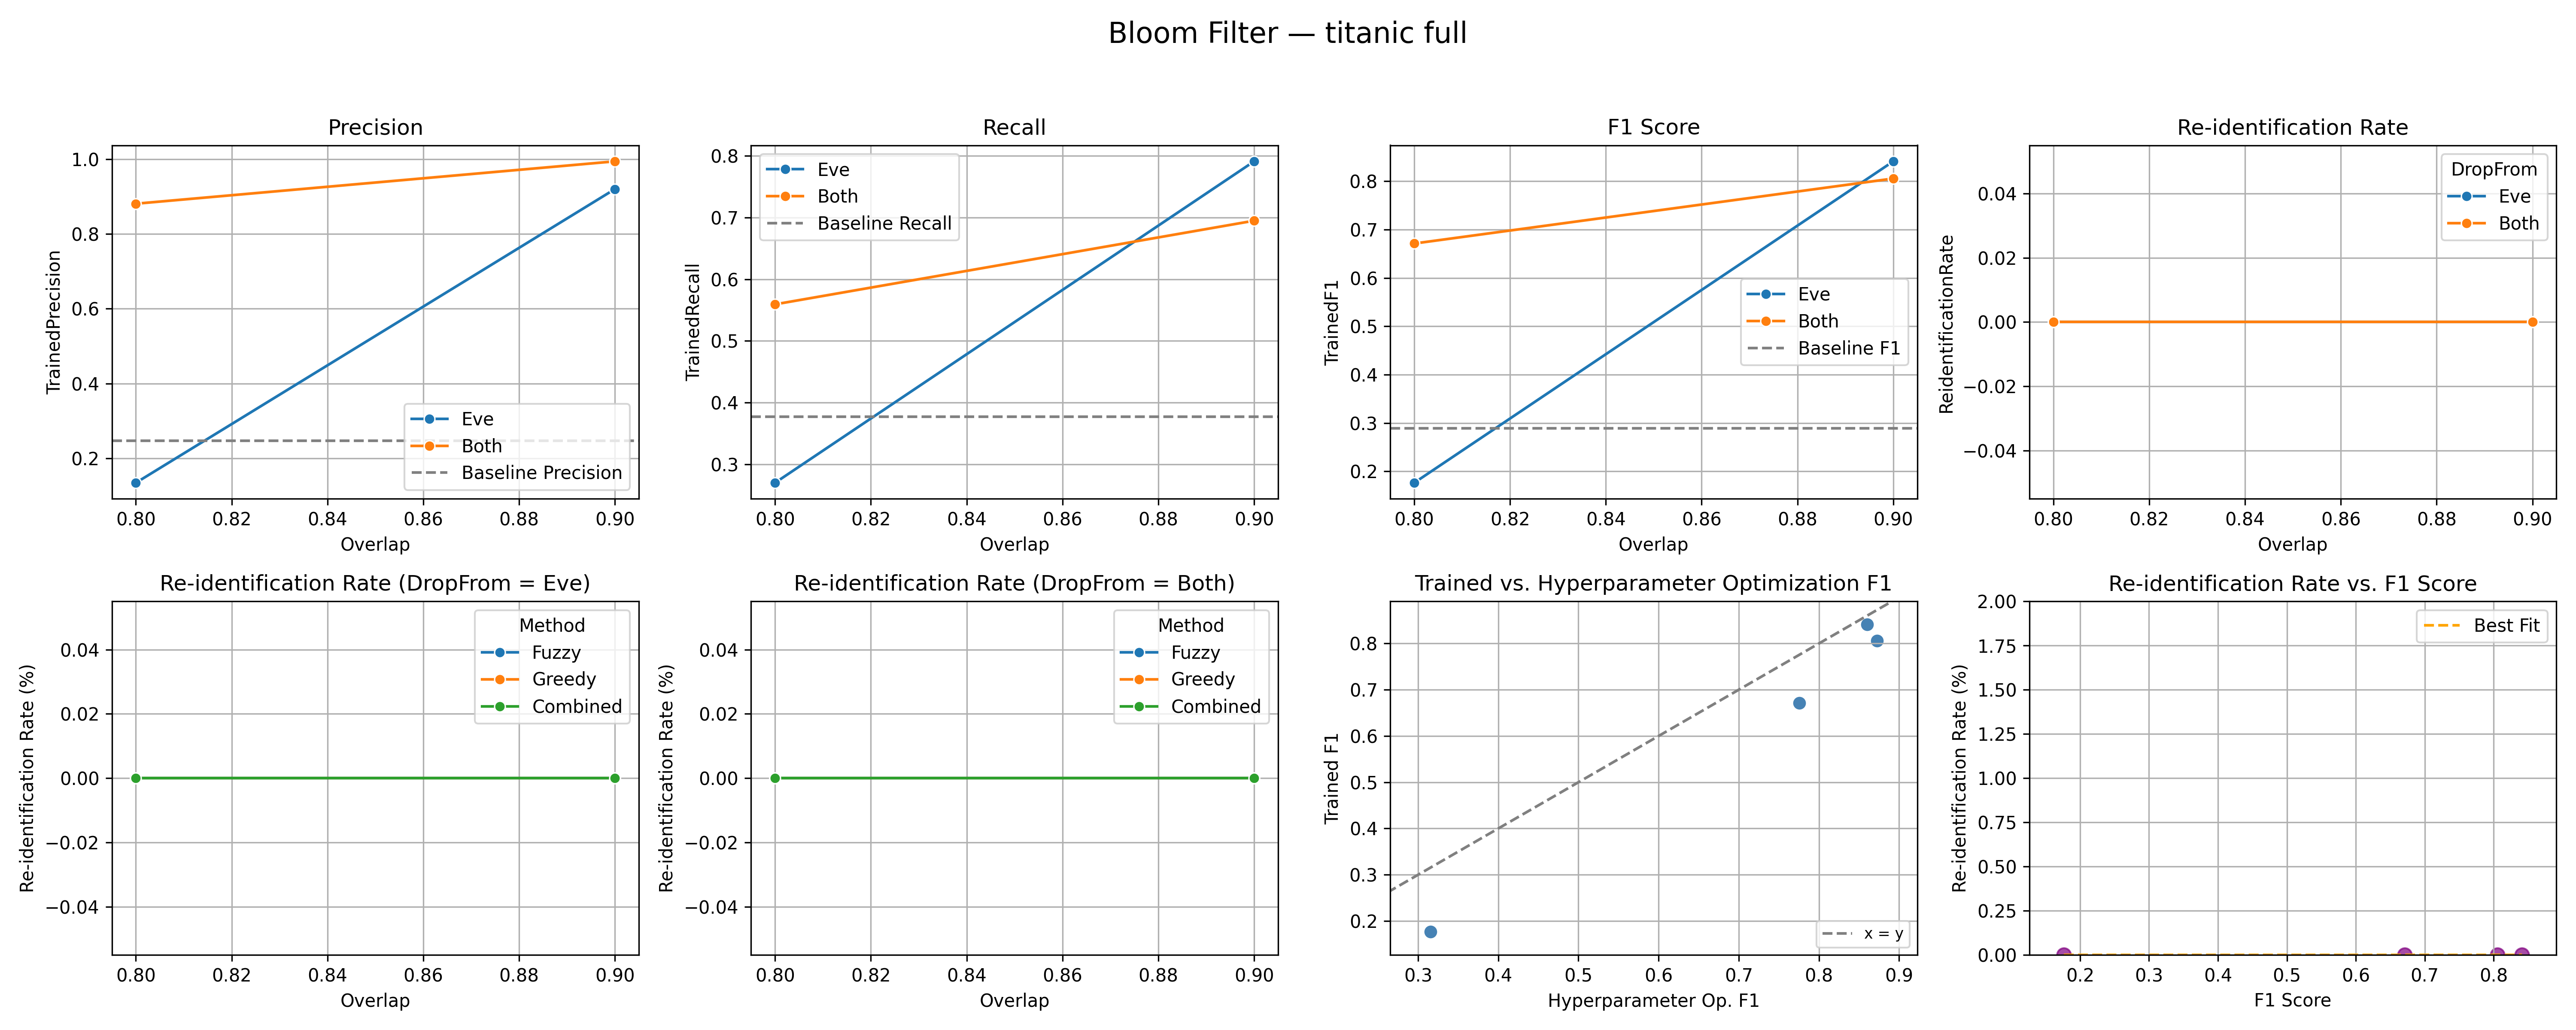
\includegraphics[width=\textwidth]{figures/BloomFilter_titanic_full_metrics.png}
    \caption{\ac{bf} results on the \texttt{titanic\_full} dataset.}
    \label{fig:bloomfilter_titanic}
\end{figure}

\begin{figure}[H]
    \centering
    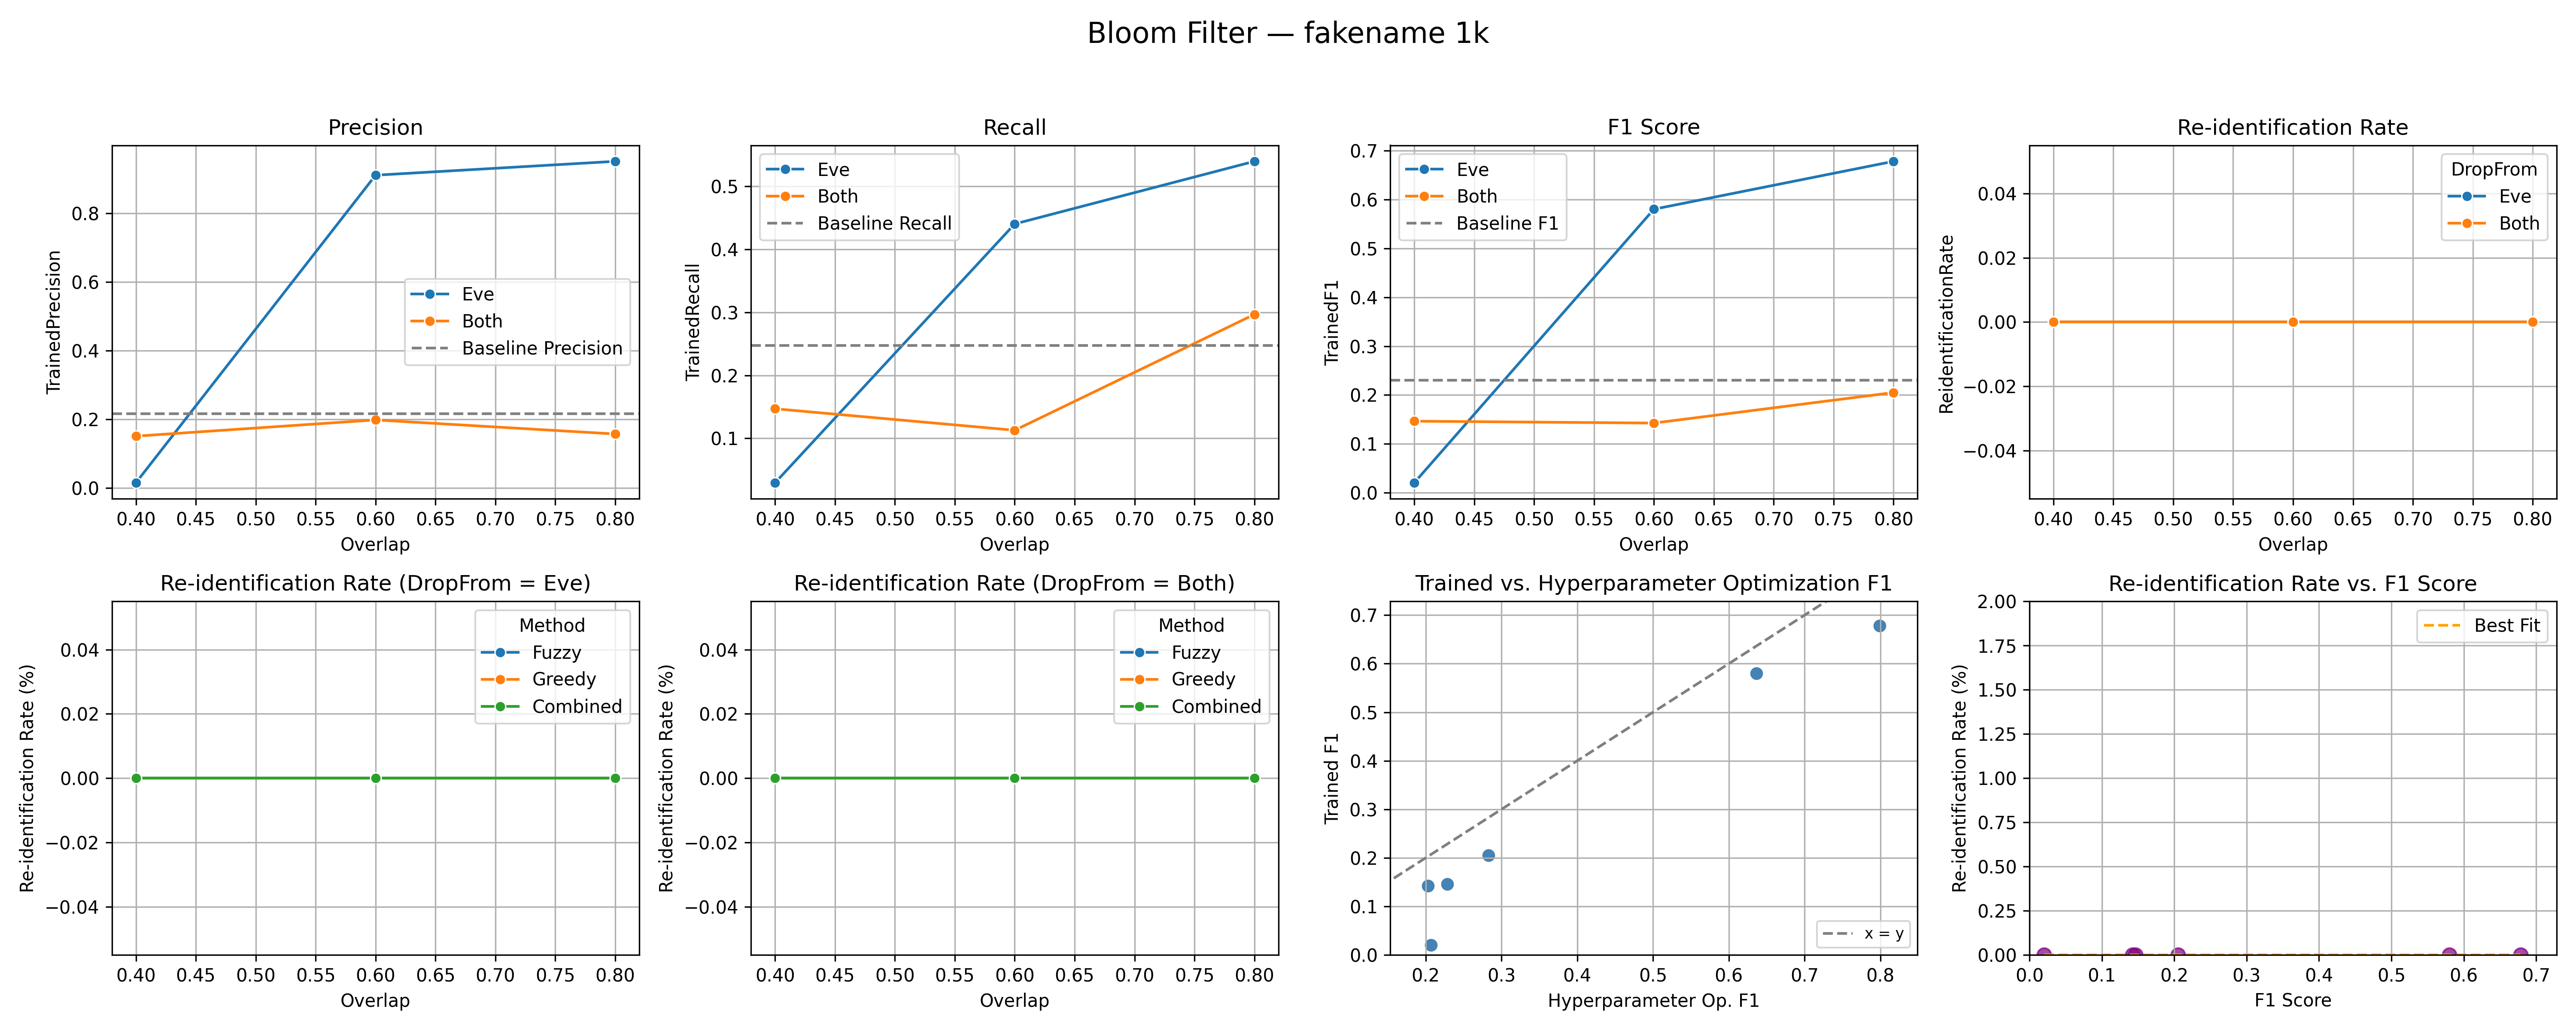
\includegraphics[width=\textwidth]{figures/BloomFilter_fakename_1k_metrics.png}
    \caption{\ac{bf} results on the \texttt{fakename\_1k} dataset.}
    \label{fig:bloomfilter_fakename1k}
\end{figure}

\begin{figure}[H]
    \centering
    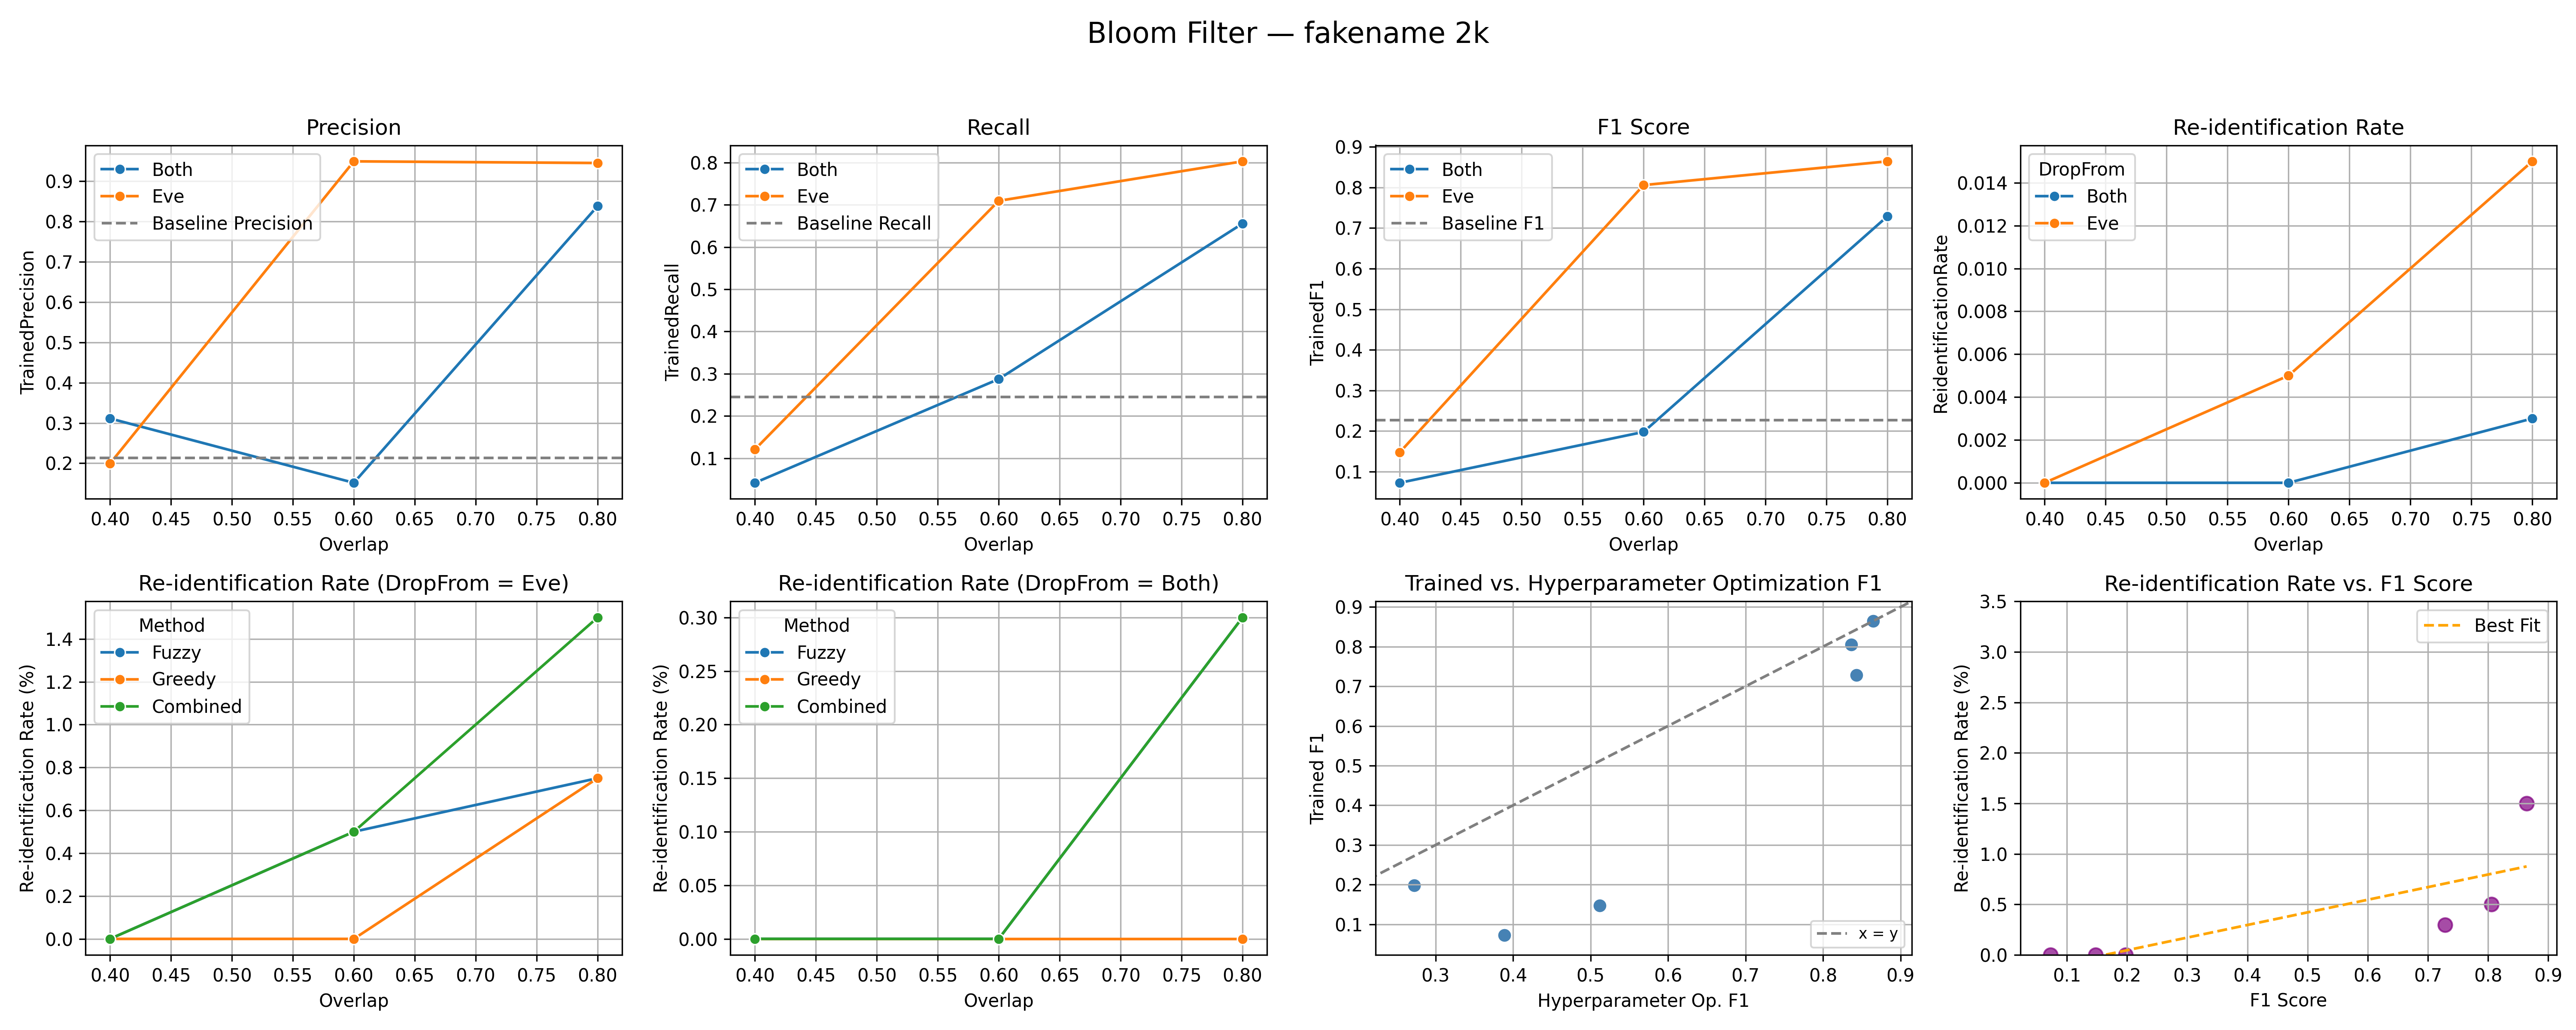
\includegraphics[width=\textwidth]{figures/BloomFilter_fakename_2k_metrics.png}
    \caption{\ac{bf} results on the \texttt{fakename\_2k} dataset.}
    \label{fig:bloomfilter_fakename2k}
\end{figure}

\begin{figure}[H]
    \centering
    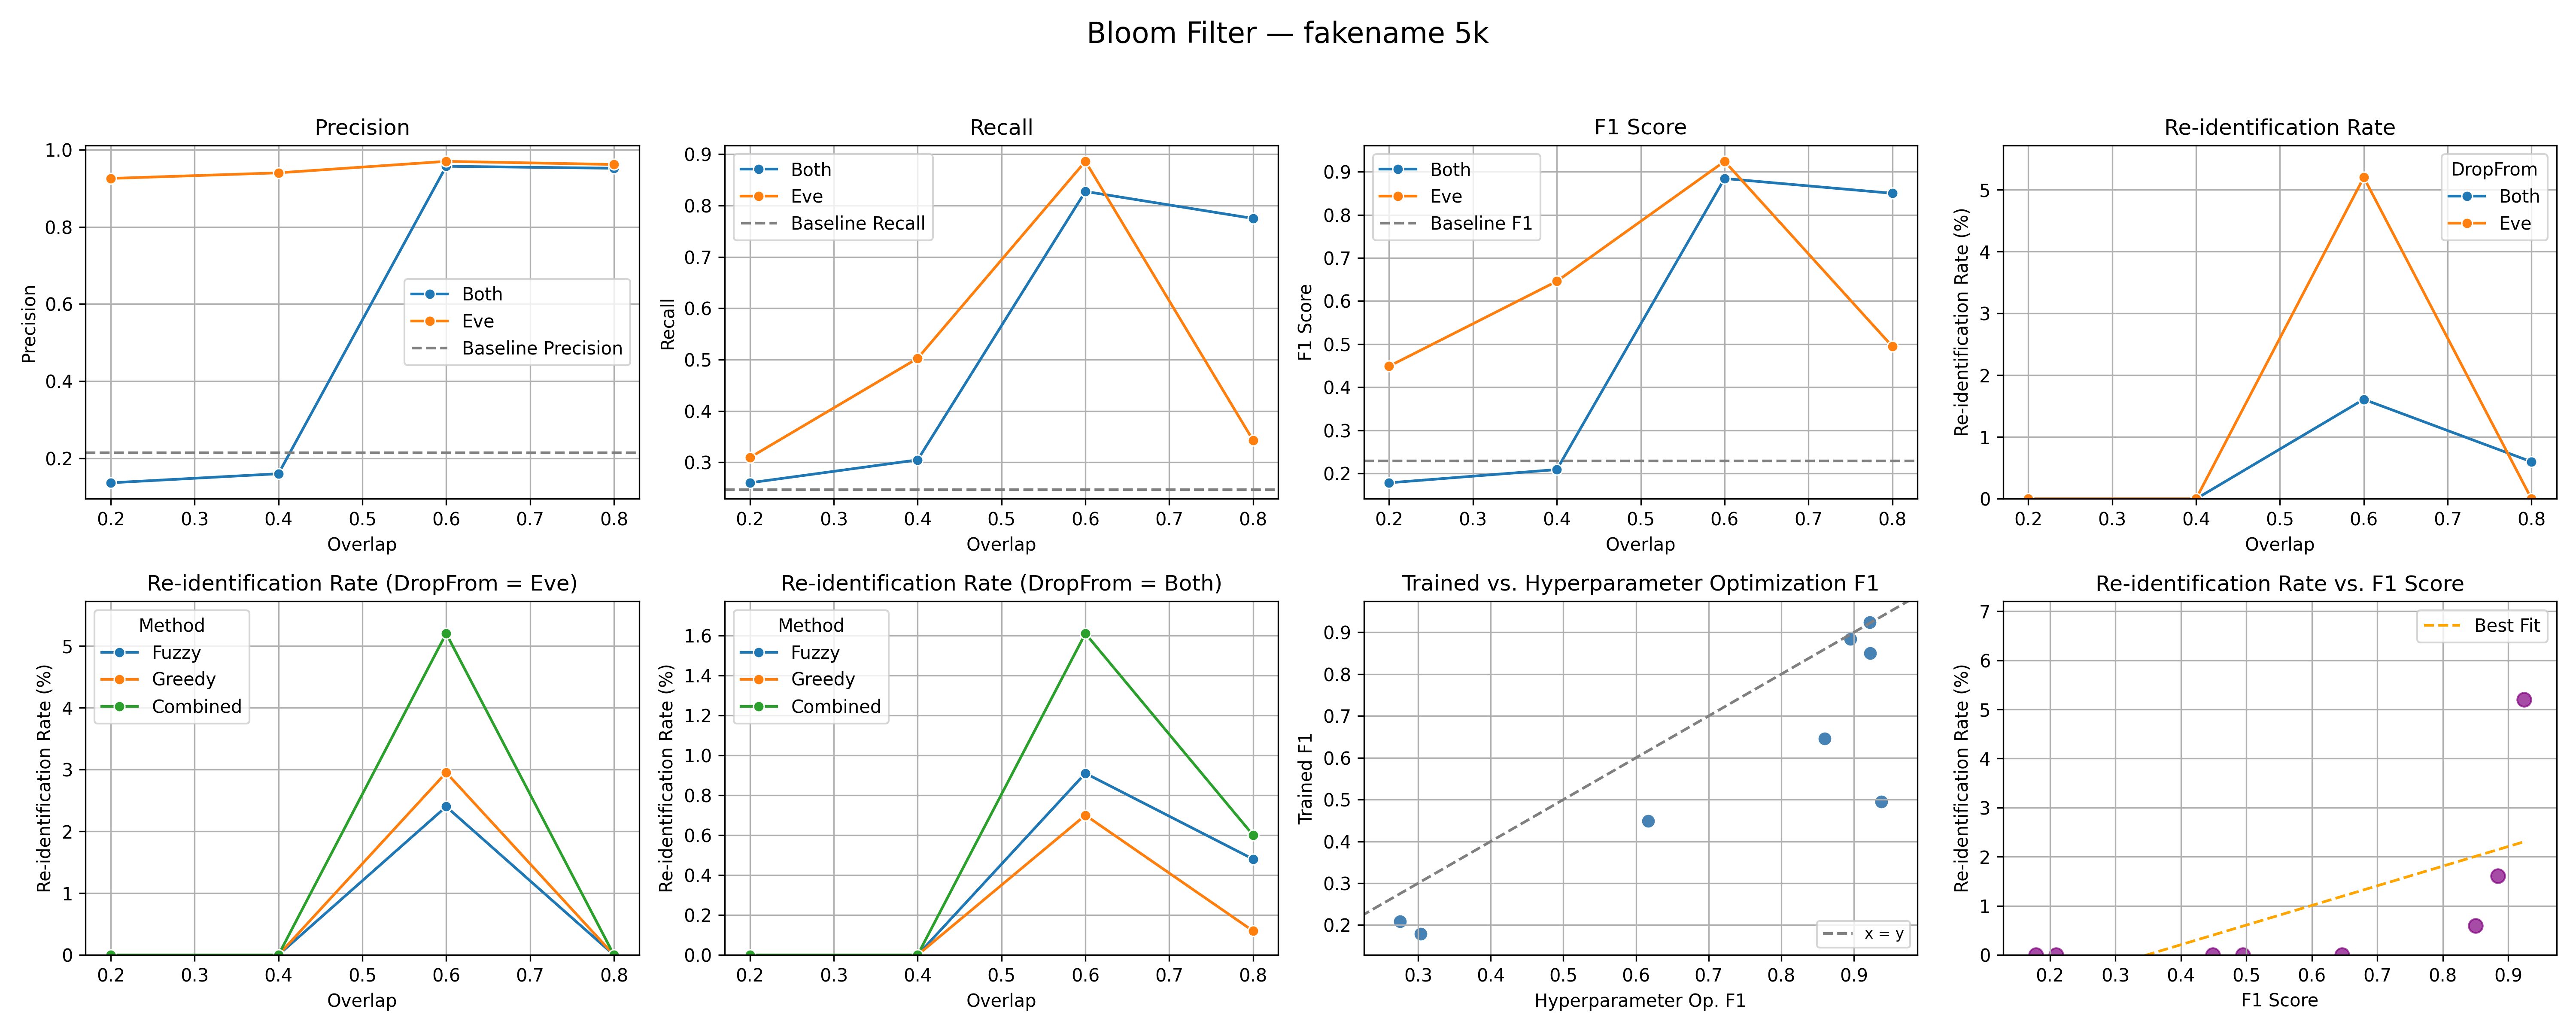
\includegraphics[width=\textwidth]{figures/BloomFilter_fakename_5k_metrics.png}
    \caption{\ac{bf} results on the \texttt{fakename\_5k} dataset.}
    \label{fig:bloomfilter_fakename5k}
\end{figure}

\begin{figure}[H]
    \centering
    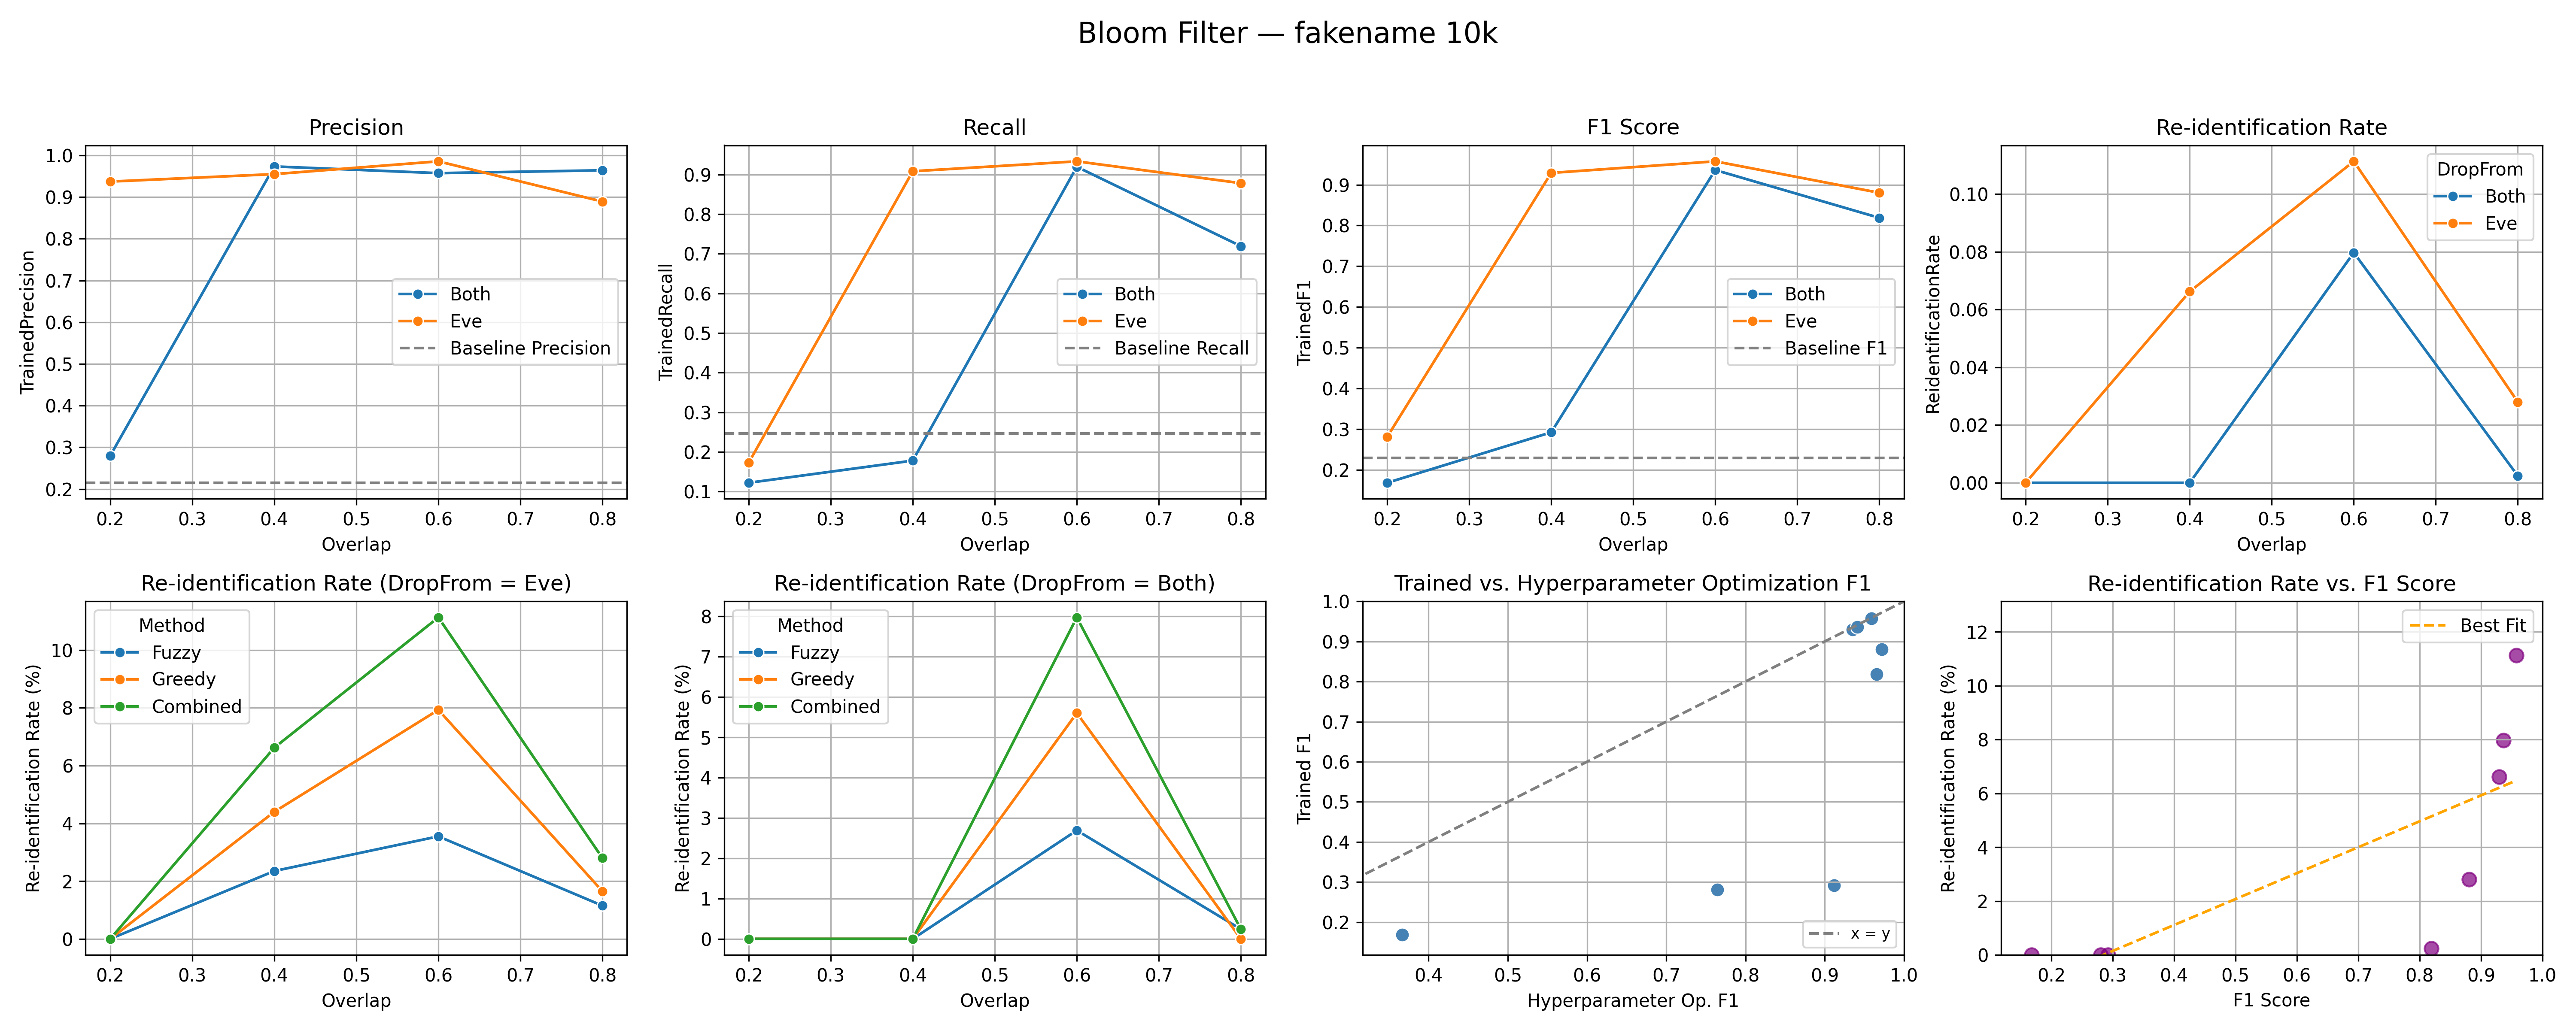
\includegraphics[width=\textwidth]{figures/BloomFilter_fakename_10k_metrics.png}
    \caption{\ac{bf} results on the \texttt{fakename\_10k} dataset.}
    \label{fig:bloomfilter_fakename10k}
\end{figure}

\begin{figure}[H]
    \centering
    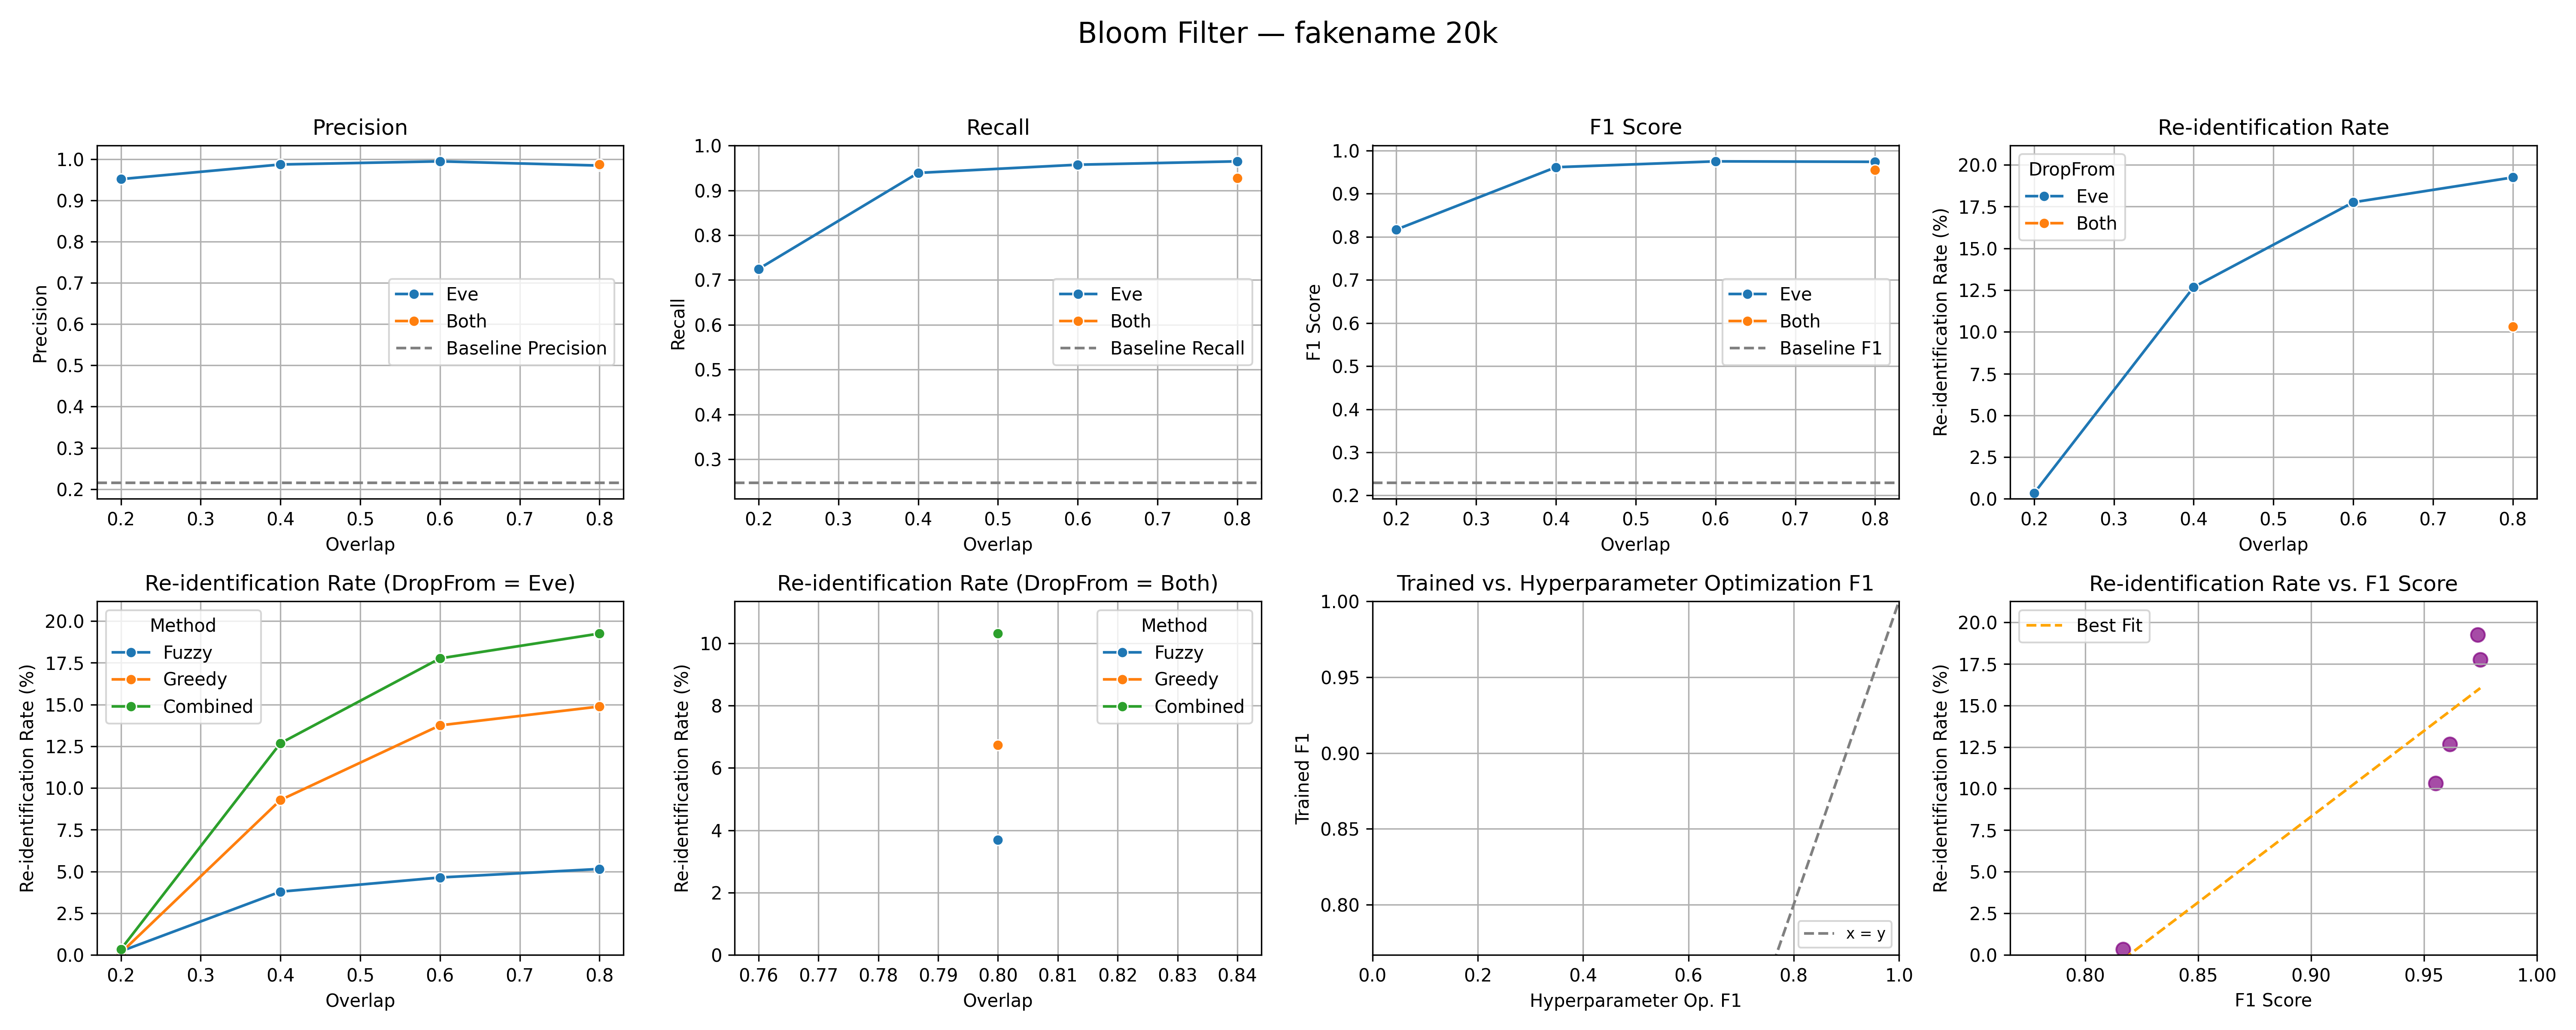
\includegraphics[width=\textwidth]{figures/BloomFilter_fakename_20k_metrics.png}
    \caption{\ac{bf} results on the \texttt{fakename\_20k} dataset.}
    \label{fig:bloomfilter_fakename20k}
\end{figure}

\begin{figure}[H]
    \centering
    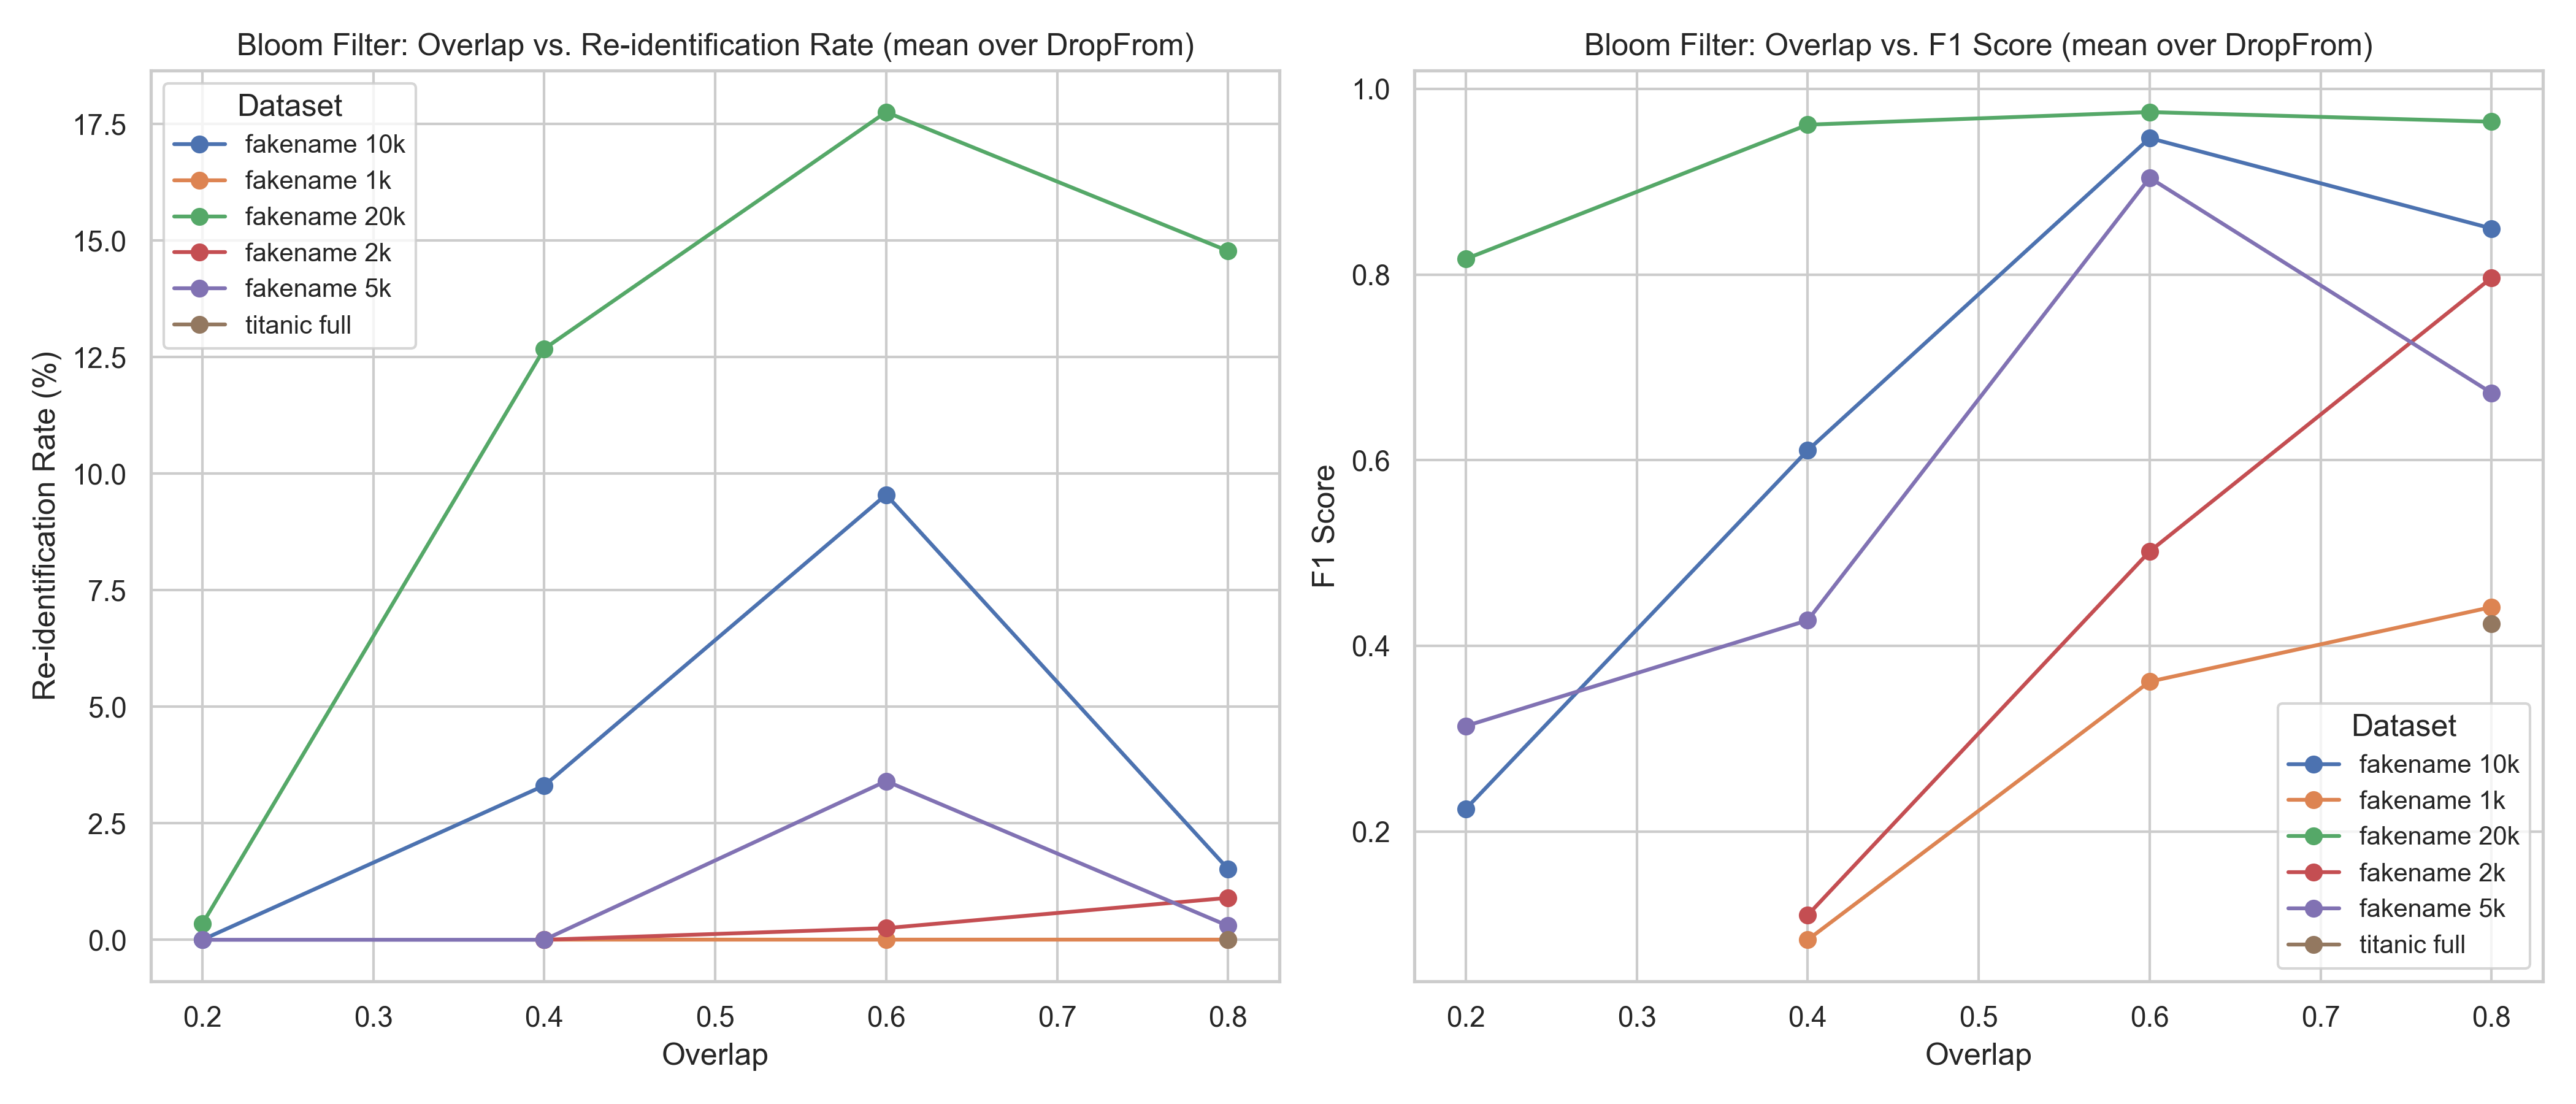
\includegraphics[width=\textwidth]{figures/BloomFilter_overlap_summary.png}
    \caption{Comparison of re-identification rates and F1 scores across all datasets with \ac{bf} encoding as a function of overlap.}
    \label{fig:bloomfilter_overlap}
\end{figure}

\begin{figure}[H]
    \centering
    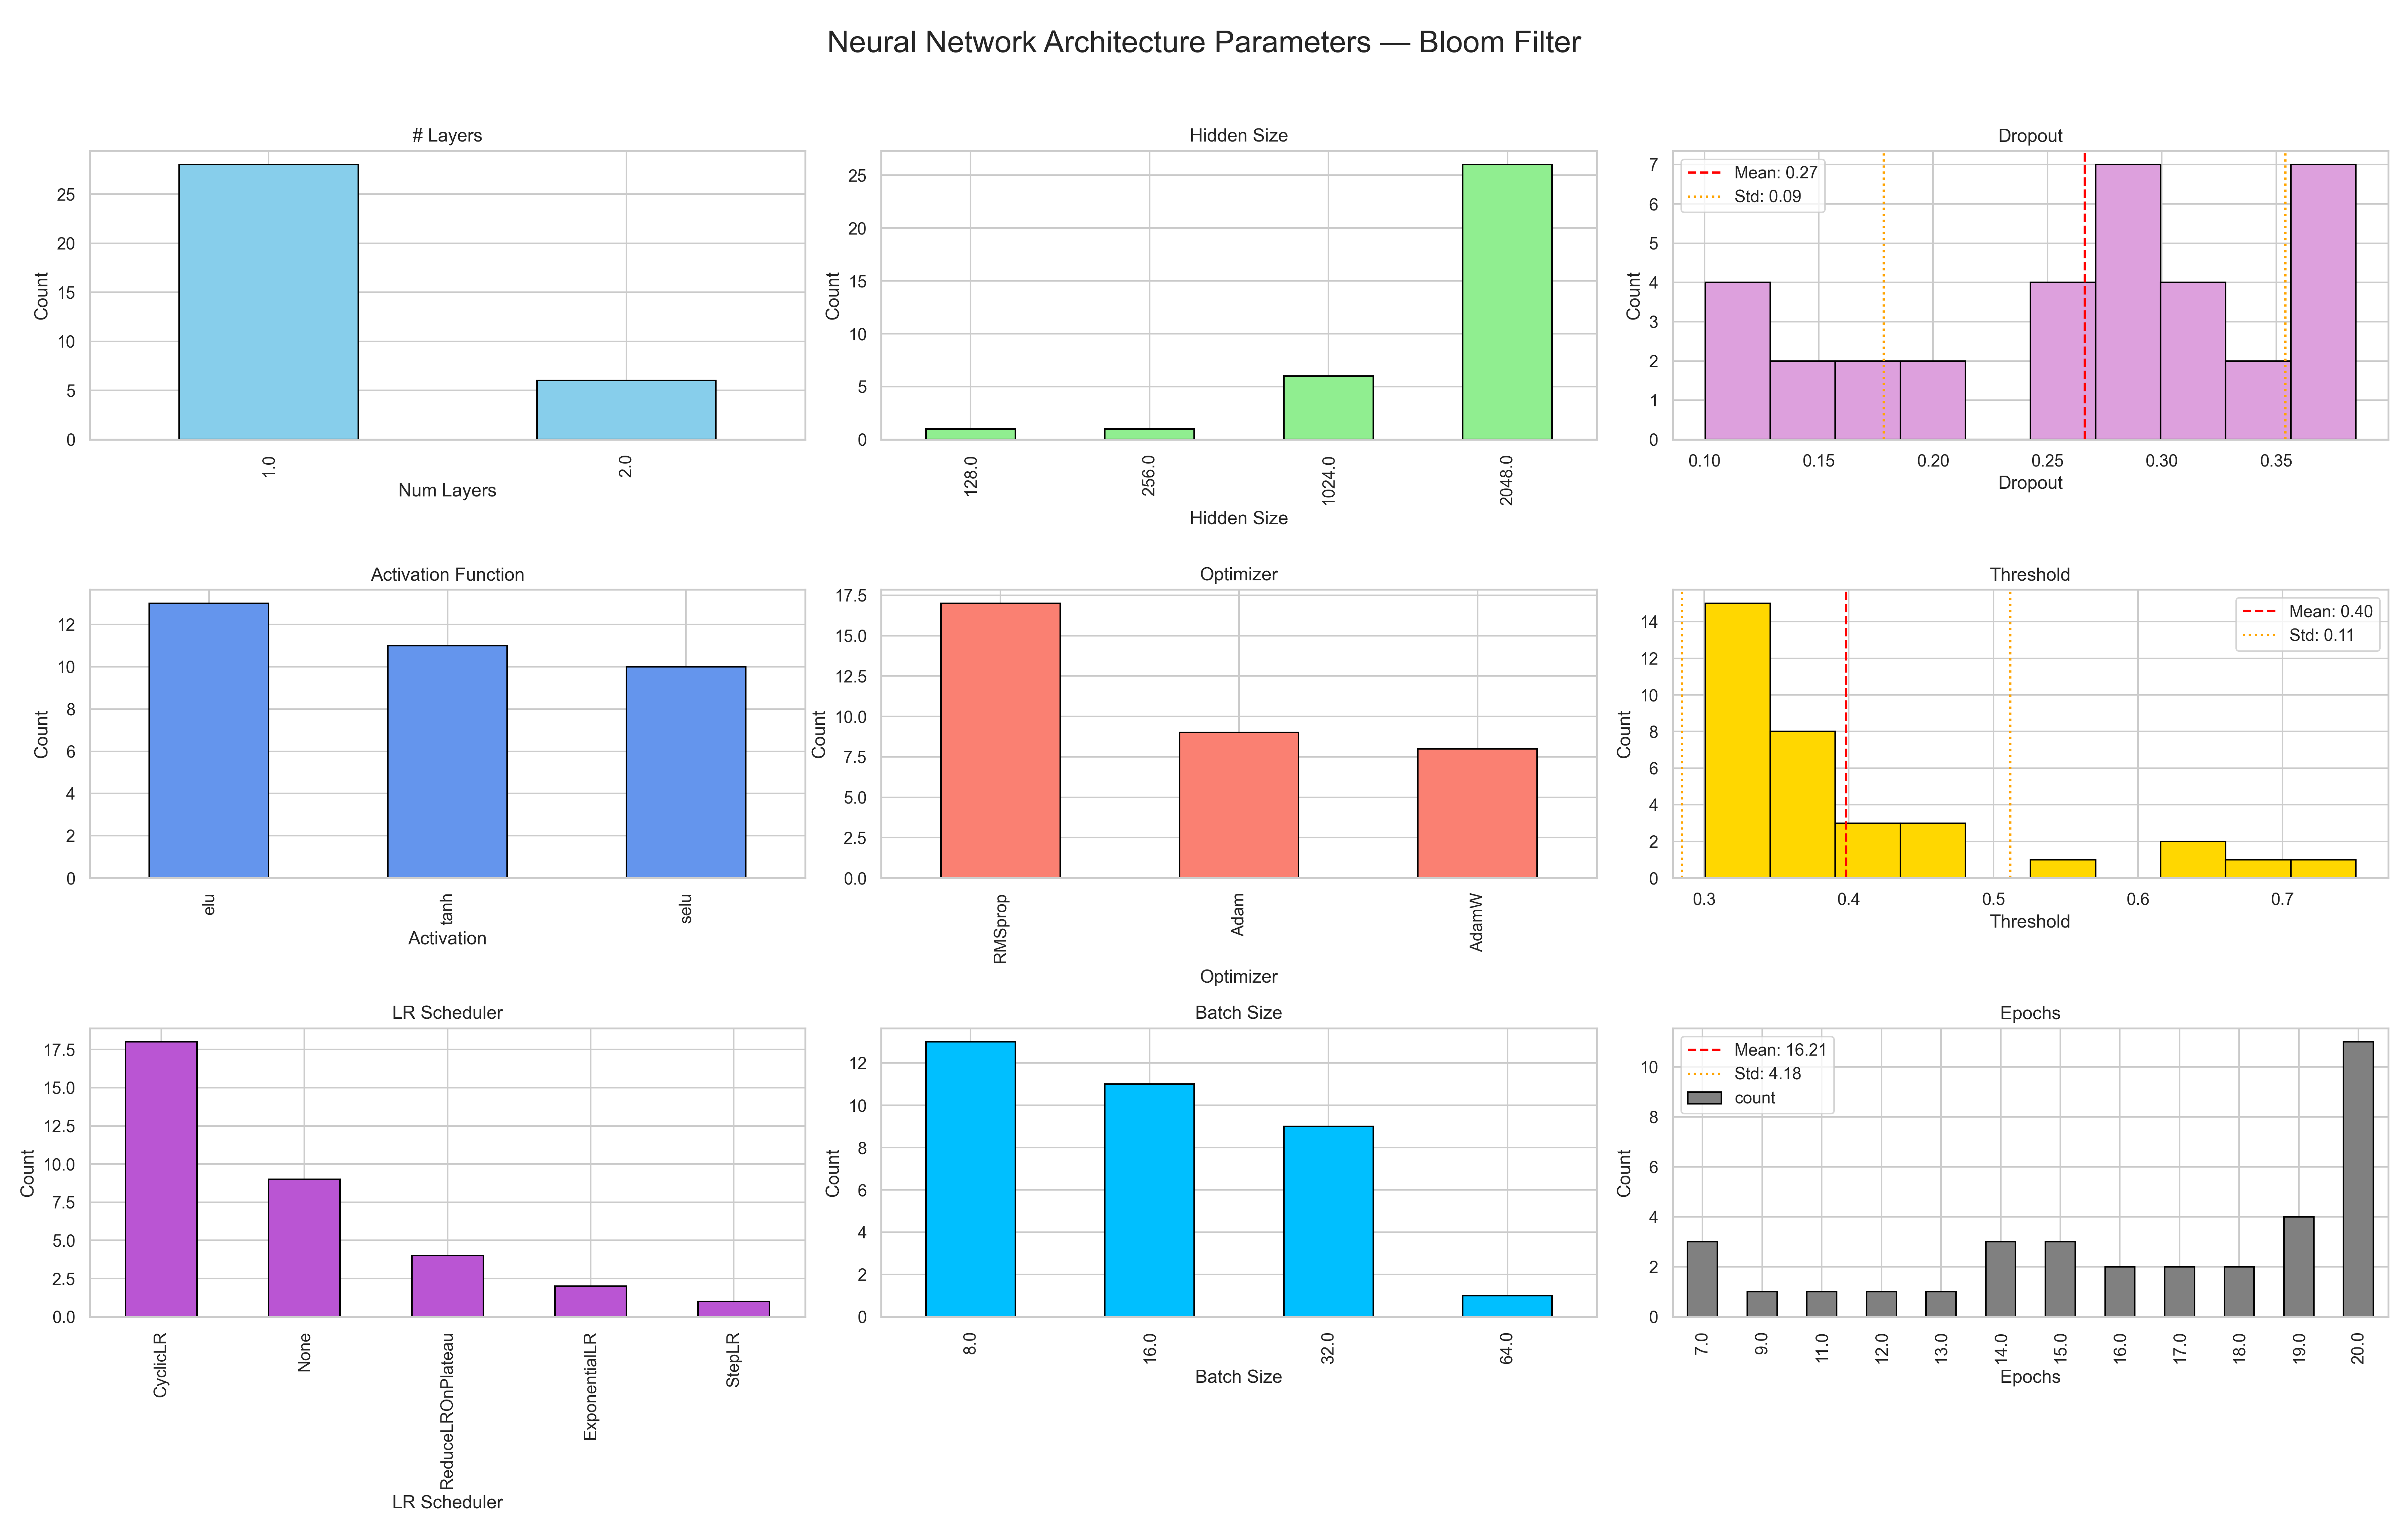
\includegraphics[width=\textwidth]{figures/BloomFilter_architecture.png}
    \caption{Distribution of selected neural network architecture parameters during hyperparameter optimization for the \ac{bf} encoding.}
    \label{fig:bloomfilter_architecture}
\end{figure}

\clearpage

\section{Encoding Scheme Comparison: \ac{dea} Results} \label{sec:encoding_comparison_results}

\begin{figure}[H]
    \centering
    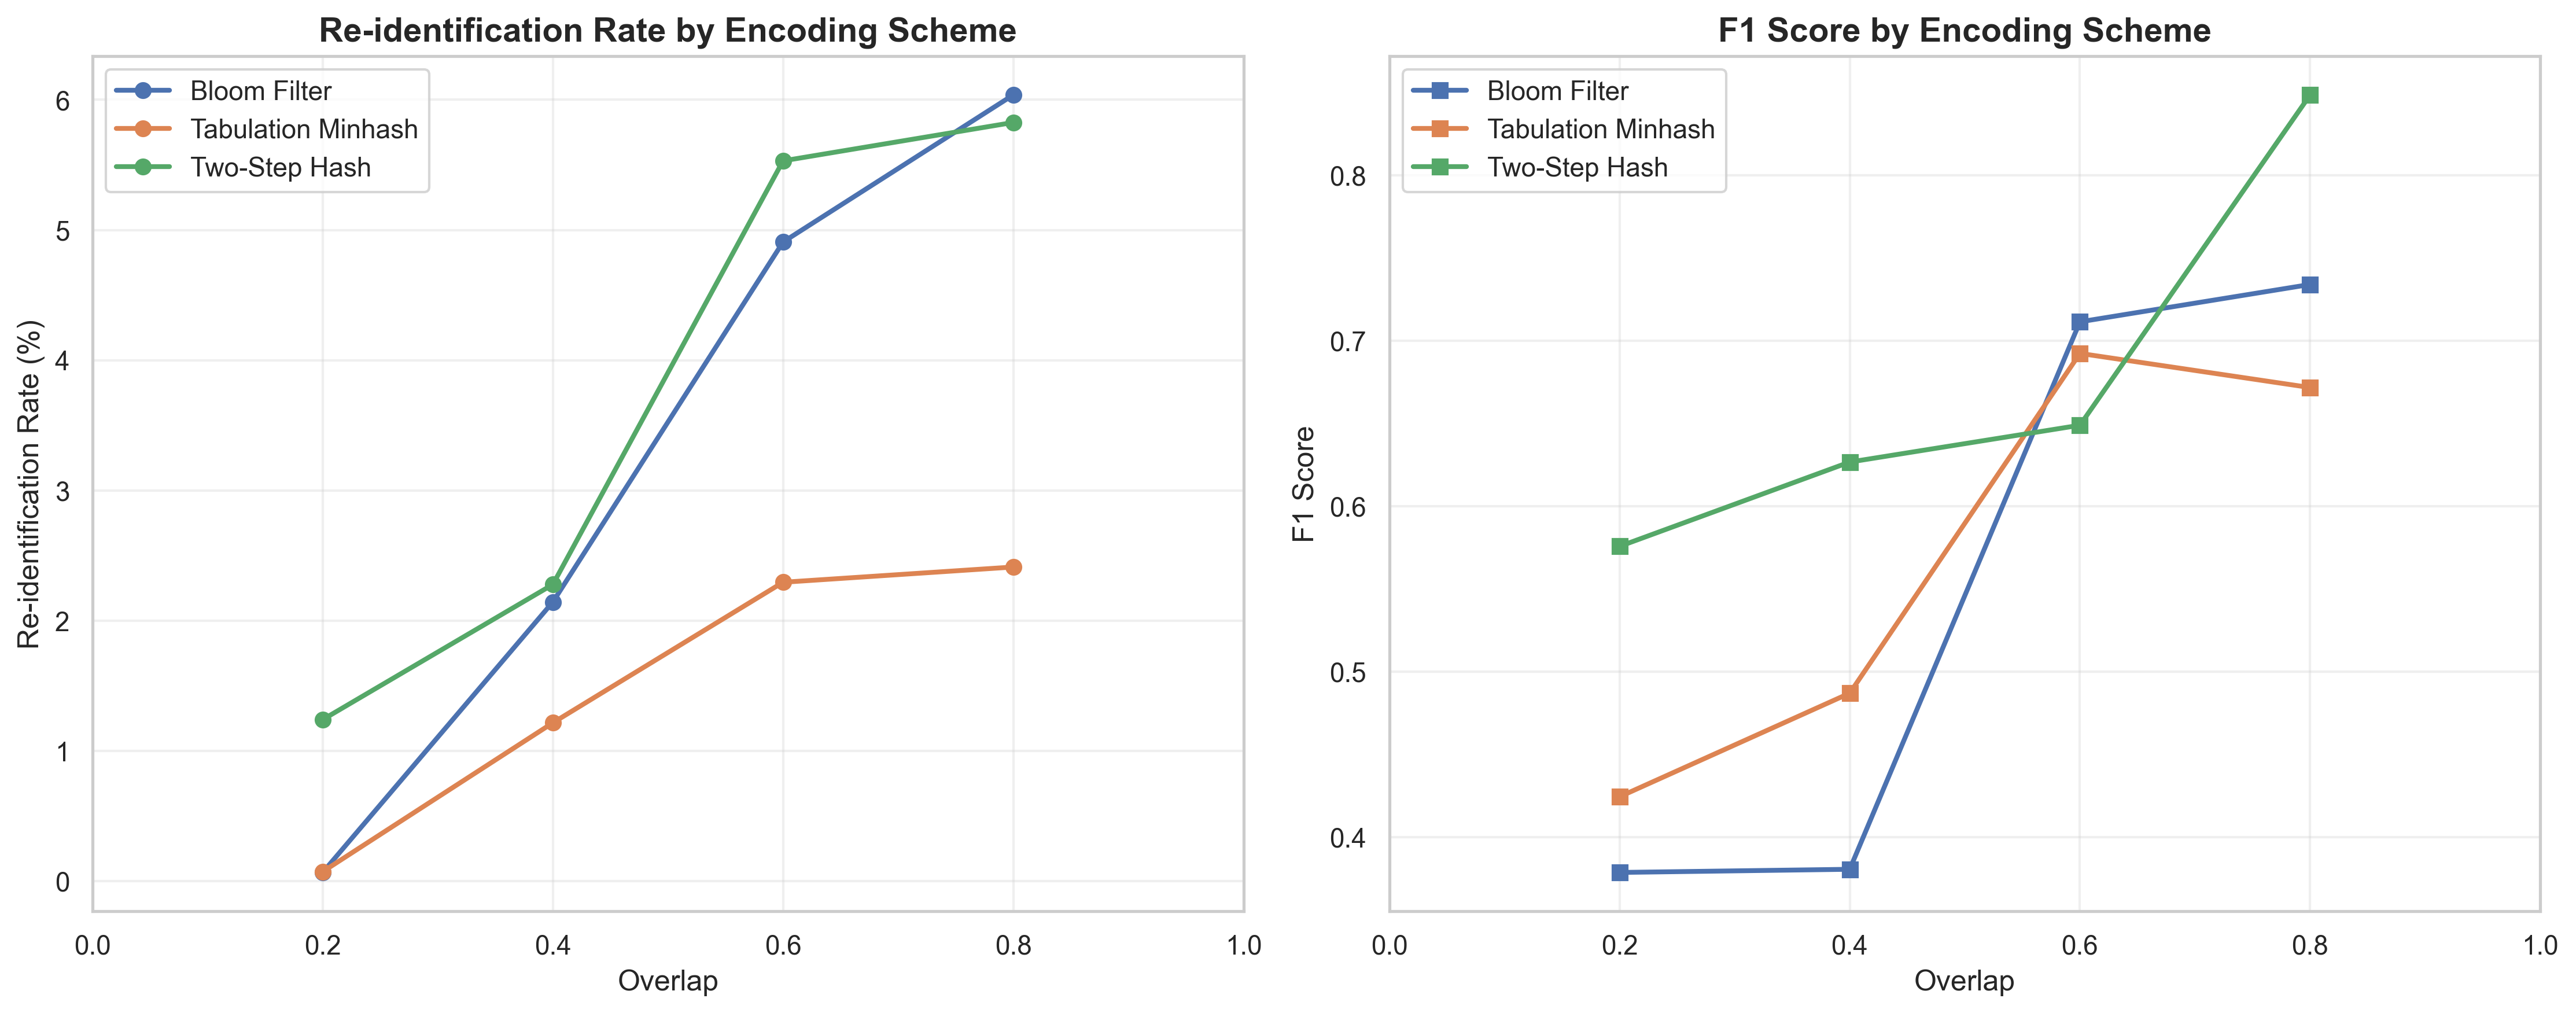
\includegraphics[width=\textwidth]{figures/dea_encoding_comparison_line_charts.png}
    \caption{Line plots of mean re-identification rate and F1 score across encoding schemes as a function of overlap.}
    \label{fig:dea_encoding_comparison_lines}
\end{figure}

\begin{figure}[H]
    \centering
    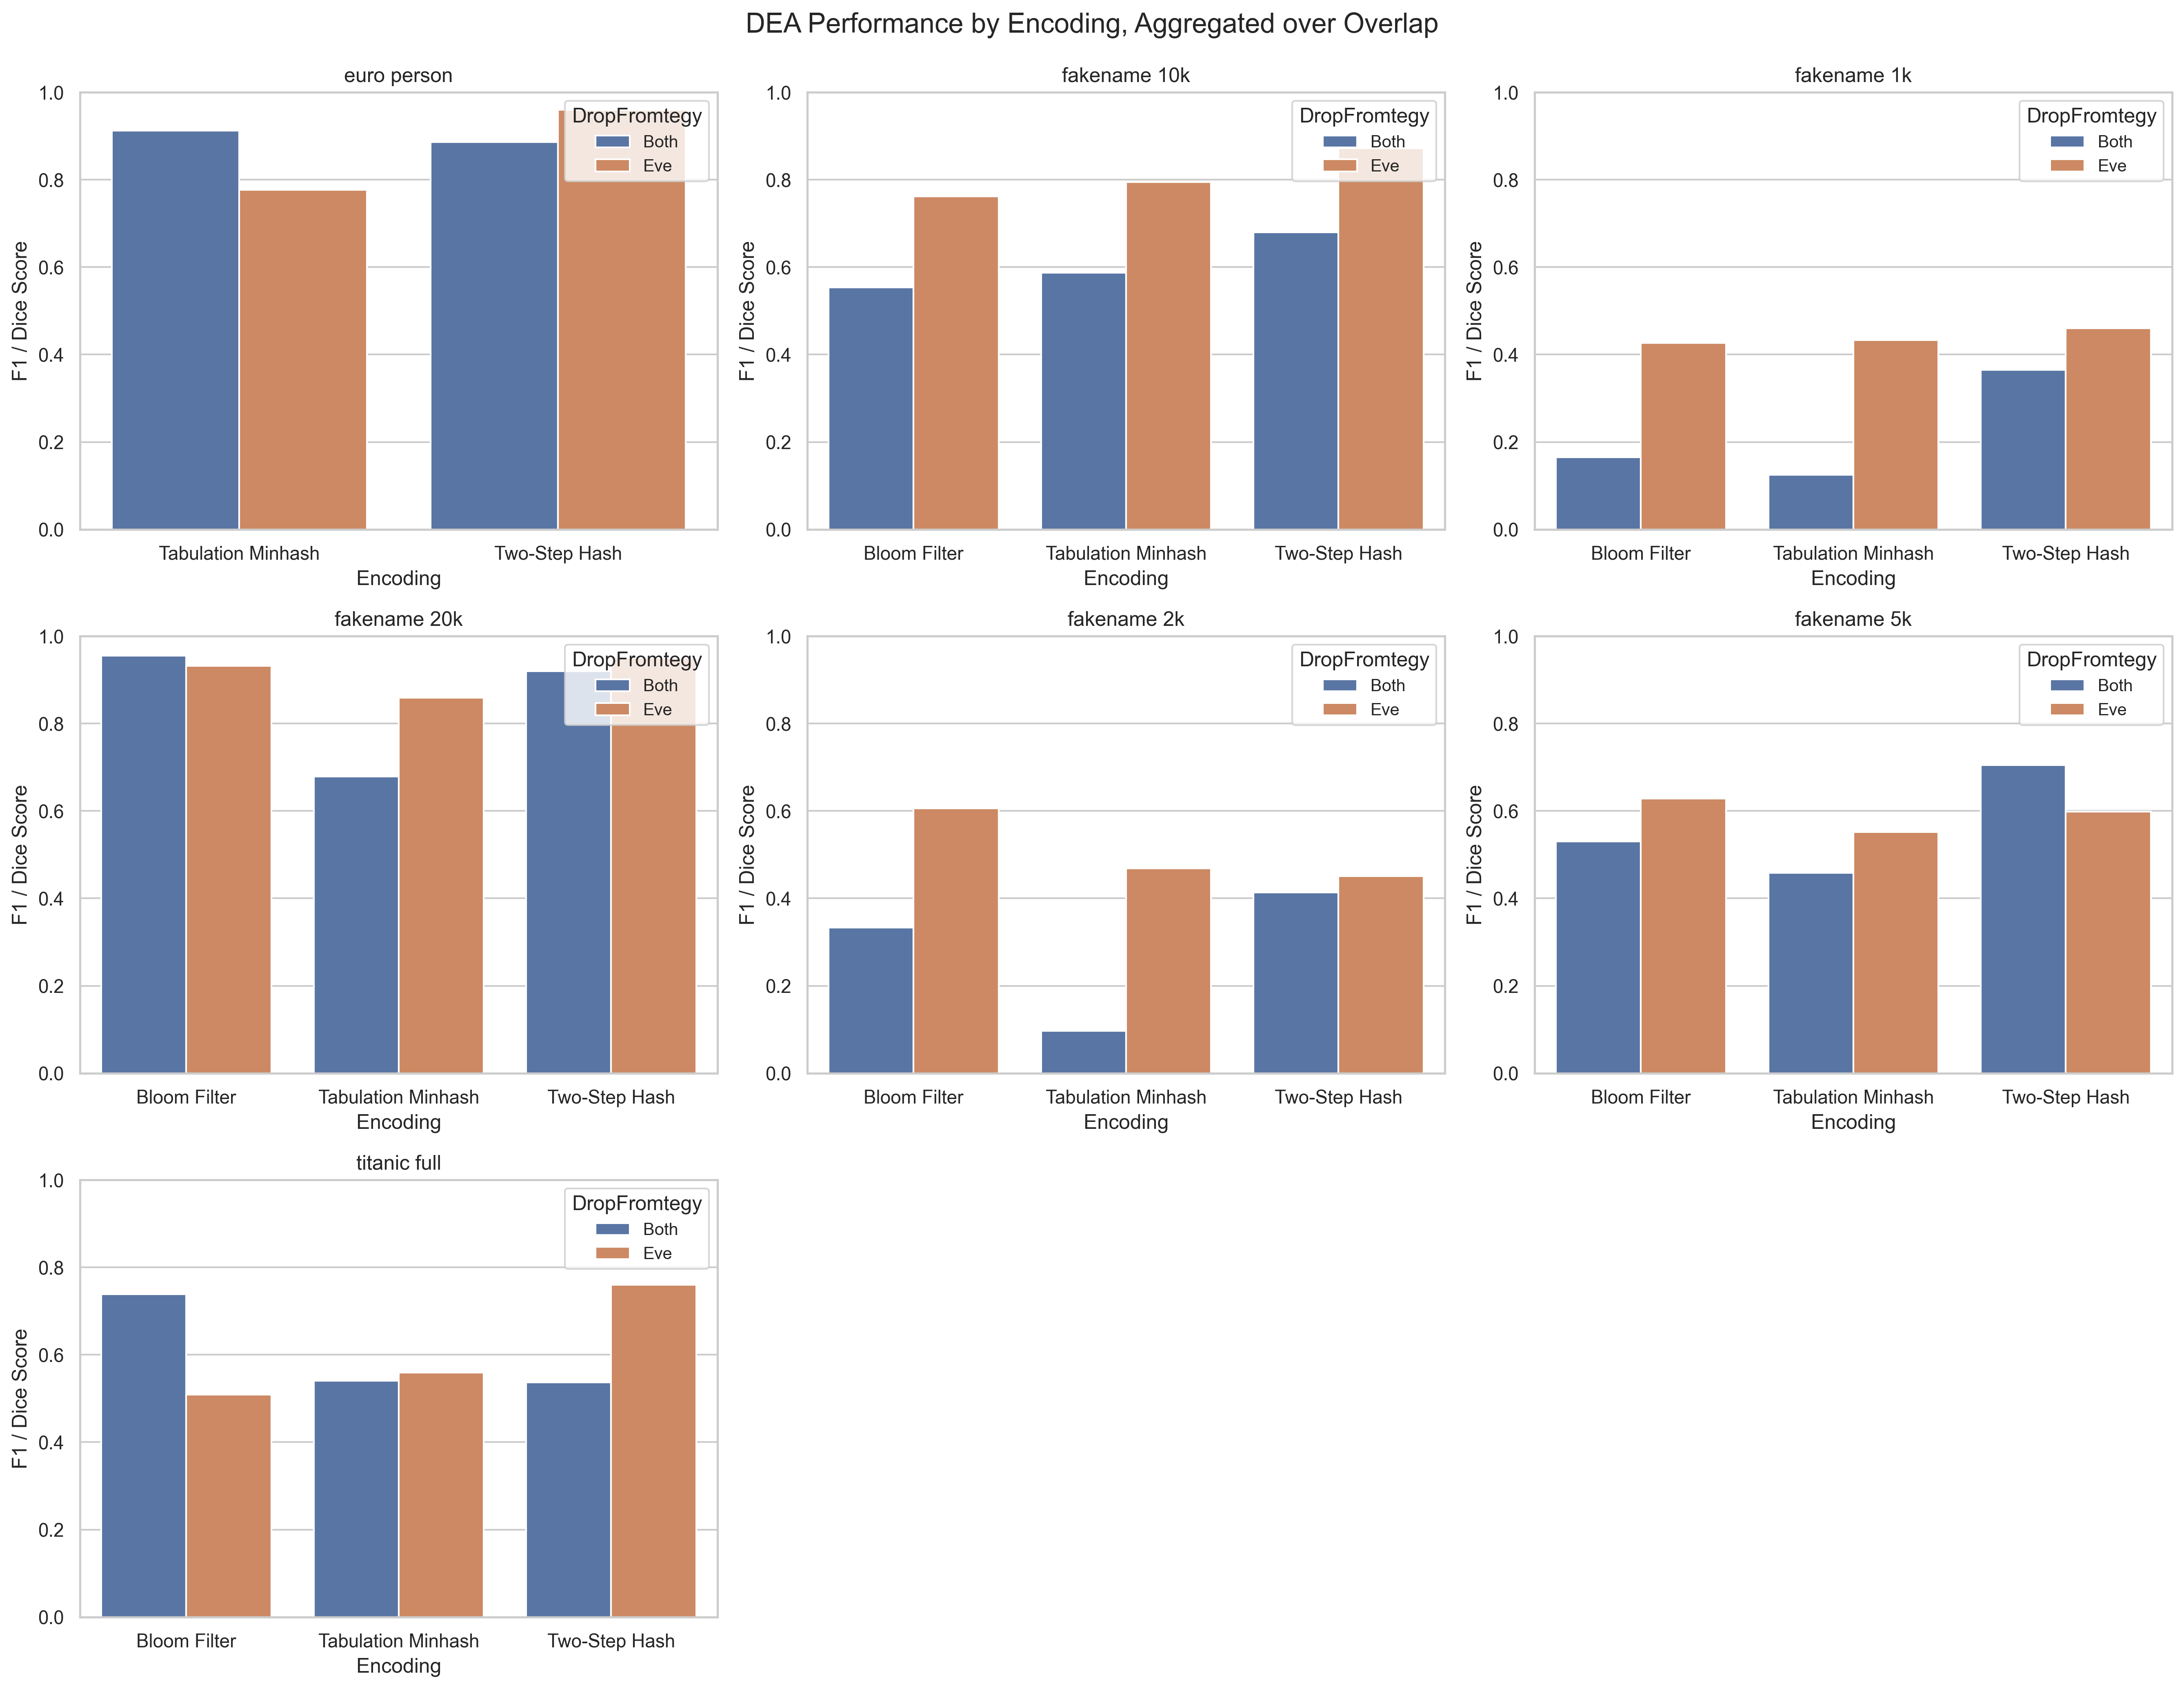
\includegraphics[width=\textwidth]{figures/dea_encoding_comparison_all_datasets.png}
    \caption{Comparison of \ac{dea} F1 scores for \ac{bf}, \ac{tmh}, and \ac{tsh} across all datasets, averaged over overlap values and separated by DropFrom strategy (Eve vs. Both).}
    \label{fig:dea_encoding_comparison_bar}
\end{figure}





